
%% 
%% Copyright 2019-2024 Elsevier Ltd
%% 
%% Version 2.4
%% 
%% Template article for cas-dc documentclass for double column output.
%% Cleaned manuscript version.
%% 

%\documentclass[a4paper,fleqn,longmktitle]{cas-dc}
\documentclass[a4paper,fleqn]{cas-dc}

%\usepackage[authoryear,longnamesfirst]{natbib}
%\usepackage[authoryear]{natbib}
\usepackage[numbers]{natbib}
\usepackage{caption}   % à ajouter dans le préambule si absent
\usepackage{booktabs}  % pour \toprule etc.
\usepackage{amsmath,amssymb}
\usepackage{amsthm}
\usepackage{graphicx}
\usepackage{longtable}
\usepackage{array}
\usepackage{pdflscape}
\graphicspath{{figs/}}
\newtheorem{definition}{Definition}

\begin{document}

\let\WriteBookmarks\relax
\def\floatpagepagefraction{1}
\def\textpagefraction{.001}

\shorttitle{Legal Query Reformulation Helps and Hurts}
\shortauthors{A. Tetereou et~al.}

\title[mode = title]{When Legal Query Reformulation Helps and Hurts: A Harm-Aware Cross-Dataset Study across BSARD and LegalBench-RAG Mini}

\author[1]{Aboudourazakou Tetereou}
\cormark[1]
\ead{aboudourazakou.tetereou@etu.uae.ac.ma}
\credit{Conceptualization, Methodology, Software, Investigation, Formal analysis, Writing -- original draft}

\author[2]{Tarik Boudaa}
\ead{t.boudaa@uae.ac.ma}
\credit{Supervision, Methodology, Validation, Writing -- review and editing}

\author[1]{Dadi El Wardani}
\ead{w.dadi@uae.ac.ma}
\credit{Supervision, Validation, Writing -- review and editing}

\affiliation[1]{
  organization={SOVIA Team, LSA, Abdelmalek Essaadi University},
  city={Tetouan},
  country={Morocco}
}

\affiliation[2]{
  organization={SDIC Team, LSA, Abdelmalek Essaadi University},
  city={Tetouan},
  country={Morocco}
}

\cortext[cor1]{Corresponding author}

\begin{abstract}
Query reformulation by Large Language Models (LLMs) often improves average retrieval metrics. However, these average gains may mask a critical risk: some individual queries are substantially degraded after reformulation. In document-centric legal retrieval, this risk takes a structural form that we call \textit{anchor loss}. Rephrasing can remove rare document identifiers such as party names, legislative references, application names or file paths. The system may then return legally coherent passages that originate from an incorrect source. Aggregated metrics alone are insufficient to characterise this failure; it must also be quantified at the level of each query, which motivates our harm-aware protocol. A manually audited conservative lexical anchor-preservation proxy is positively associated with $\Delta$Recall@100 after query-clustered inference ($\rho=0.179$, $p_{\mathrm{Holm}}=0.0012$). We conduct a comparative study on BSARD and a subset of LegalBench-RAG mini. BM25 provides the primary controlled lexical framework, complemented on LegalBench-RAG mini by exact dense retrieval with E5 and BGE and by fixed-weight BM25+dense hybrid baselines. We compare direct query replacement, reciprocal rank fusion preserving the original query (RRF), and a non-learning consensus weighting method, the Retrieval Consensus Score (RCS). The results show that HyDE-style replacement is unsafe even in statutory retrieval: on BSARD, DeepSeek and GPT HyDE reduce Recall@100 by 0.112 and 0.077, respectively, and both losses remain significant after Holm correction. The corresponding original-preserving RRF variants reduce these changes to $+0.009$ and $-0.004$, with no significant degradation. On LegalBench-RAG mini, LLM replacement can cause Recall@100 to drop by more than half, with an even steeper decline for HyDE-style reformulations. A chunk-only ablation shows that filepath-aware indexing amplifies this failure mode but does not fully create it: HyDE-style replacement remains significantly harmful, while original-preserving fusion continues to improve Recall@100 without filepath metadata. Harmful replacement also persists beyond BM25 in the tested filepath+chunk setting: GPT keyword and HyDE significantly degrade E5, BGE and hybrid retrieval. Dense-only original-preserving fusion yields positive mean Recall@100 gains with low harm rates, although these recall gains are not significant; under hybrid BGE, original + DeepSeek keyword + GPT legal rewrite improves Recall@100 by 0.054 with only 1.0\% of queries degraded and significant gains in Recall@10, Recall@100 and nDCG@10. On BSARD, original-preserving keyword fusion improves Recall@100 with only 0.45\% of queries degraded. The RCS improves top-of-list ranking by favouring documents supported by multiple reliable reformulation views. These results support a clear operational principle: preserve the original query as an anchor and use LLM reformulations as controlled auxiliary views.
\end{abstract}
\begin{highlights}
\item We evaluate LLM query reformulation across statutory and document-centric legal retrieval tasks.
\item A manually audited anchor-preservation proxy is positively associated with Recall@100 changes under direct replacement.
\item HyDE-style replacement significantly reduces Recall@100 on BSARD; on LegalBench-RAG mini, GPT keyword and HyDE degradation persists under BM25, E5, BGE and hybrid retrieval.
\item Original-preserving RRF stabilises dense retrieval and significantly improves Recall@100 under hybrid BGE retrieval.
\item Retrieval Consensus Score improves early ranking by rewarding agreement across reliable reformulation views.
\end{highlights}
\begin{keywords}
legal information retrieval \sep
legal retrieval-augmented generation \sep
query reformulation \sep
large language models \sep
reciprocal rank fusion \sep
Retrieval Consensus Score \sep
harm-aware evaluation \sep
anchor preservation
\end{keywords}
\maketitle
\section{Introduction}
Information retrieval is the first link in the chain of reliability for legal systems based on retrieval-augmented generation (RAG). Before a language model can cite a section of legislation, identify a contractual clause or substantiate a response regarding a privacy policy, a retrieval component must locate the exact passages that underpin that response. When this step fails, the generation process inherits a problem of missing evidence: even a linguistically rigorous model can produce a plausible but legally unfounded response, without the user being made aware of it. Legal retrieval therefore warrants direct evaluation, rather than being treated as a silent pre-processing step in an end-to-end pipeline.
In this context, query reformulation by large language models (LLMs) emerges as a promising strategy. By aligning the user’s wording with the vocabulary of the target documents, it can reduce lexical mismatch and improve average retrieval performance (Ma et al., 2023; Jagerman et al., 2023; Zhu et al., 2023). This approach is particularly relevant in law: users often formulate their needs in everyday language, whereas legislative, contractual or regulatory texts adhere to precise terminology. An LLM can thus enrich an under-specified query with legal terms likely to improve lexical alignment with the reference documents.
What remains less studied is not only whether reformulations improve average scores, but also when they degrade certain queries, why such degradations occur, and how to design a pipeline that mitigates this risk. This issue is all the more central in law because certain terms in a query are not merely descriptive: they identify the source to be queried.
In document-centric legal retrieval, these terms act as document anchors. They may include names of parties, document titles, legislative references, application names, file paths or other rare identifiers that link the query to a specific source. A query concerning a non-disclosure agreement between two named parties does not merely seek a clause relating to confidentiality; it seeks that clause in that specific contract. If a reformulation replaces these identifiers with generic terms such as ``confidentiality'', ``non-disclosure obligations'' or ``proprietary information'', the system may return a legally coherent clause but one taken from the wrong document. The failure is then not a lack of thematic relevance, but a source error. We call this mechanism \textit{anchor loss}, and we show that it is a central failure mode of replacement-based reformulation in the document-centric setting studied here. A chunk-only ablation further shows that source-aware filepath indexing amplifies this mechanism, without fully creating it.
This finding warrants a reassessment of the role of the original query in legal retrieval pipelines. In many systems, reformulation is used as a pre-processing step capable of replacing the initial query prior to retrieval. We investigate the opposite hypothesis: the original query must be preserved as a retrieval branch, whilst LLM reformulations must be used as auxiliary views. This distinction—replacement versus preservation—is the crux of our study. It addresses a practical deployment decision: should the LLM be entrusted with the responsibility of completely rewriting the search intent, or should the user’s formulation be retained as a document anchor?
We examine this question primarily within a BM25 lexical retrieval framework. This choice is deliberate: BM25 remains a robust, transparent and widely used benchmark in information retrieval, and it allows us to isolate the effect of reformulation on the correspondence between queries, rare terms and documents. We then complement the LegalBench-RAG mini experiments with exact dense retrieval using E5 and BGE, as well as fixed-weight BM25+dense hybrids, to test whether harmful replacement and the preservation principle persist beyond lexical matching. Our experiments cover two complementary benchmarks. BSARD evaluates the retrieval of legislative articles in French, where reformulation can enrich the query with useful legal vocabulary. LegalBench-RAG mini evaluates a more document-centric retrieval setting on contracts and privacy policies, where preserving document anchors becomes crucial.
We compare three query-use strategies. The first directly replaces the original query with an LLM reformulation. The second preserves the original query using reciprocal rank fusion (RRF), in which both the initial query and the reformulations contribute to the final list of results. The third uses the Retrieval Consensus Score (RCS), a consensus-based weighting strategy without training that favours documents retrieved by multiple reliable reformulation views. These strategies are evaluated primarily with BM25 and, on LegalBench-RAG mini, through dense and hybrid robustness checks. Our aim is not merely to measure average gains, but to assess the robustness of each strategy at the level of individual queries.
The evaluation is therefore sensitive to performance degradation on a per-query basis. In addition to standard retrieval metrics, we report per-query degradation rates, i.e. the proportion of queries for which a strategy degrades performance compared to the original query. This measure is essential in law: a method that slightly improves the average may still be unacceptable if it significantly degrades certain critical queries. We complement this analysis with bootstrap confidence intervals, paired statistical tests and a Holm correction for multiple comparisons.
Our contributions are as follows:
\begin{enumerate}
    \item We propose a degradation-sensitive evaluation protocol for LLM query reformulation in legal retrieval, combining aggregate metrics, per-query harm rates and corrected statistical tests.
    \item We show that direct query replacement can remove or dilute source-identifying information in document-centric tasks, leading to severe degradation and potentially to legally coherent passages from incorrect sources.
    \item We provide a manually audited, conservative lexical proxy for document-identifier preservation and show a significant query-clustered association with Recall@100 changes, while distinguishing this diagnostic from a complete APR benchmark or causal proof.
    \item We demonstrate across BSARD and LegalBench-RAG mini that preserving the original query is more robust than direct replacement. This principle is supported under BM25, yields low-harm positive mean gains in dense-only fusion, and produces significant recall gains under hybrid BGE retrieval; consensus among reliable views can additionally improve top-of-list ranking.
\end{enumerate}
\section{Related work}

\subsection{Legal information retrieval and legal RAG}

Legal information retrieval differs from general-purpose search
in that thematic relevance is not sufficient: the passages
retrieved must come from the legally correct source. In
retrieval-augmented generation (RAG) systems, this
requirement is critical — an error in the source directly becomes an
error in attribution or citation (Lewis et al., 2020).

Two retrieval profiles underpin this study.
\textit{Statutory retrieval} involves identifying the
legal provision relevant to a query. BSARD illustrates this profile: the corpus
links legal questions in French to Belgian statutory provisions
annotated by legal experts, within a corpus of over
22,600 provisions (Louis and Spanakis, 2022). The main difficulty
is the lexical gap between the user’s everyday language and the
technical terminology of the texts. \textit{Document-centric retrieval}
poses a different problem. In tasks
involving the analysis of contracts, merger and acquisition agreements or
privacy policies, several documents may contain clauses
that are thematically similar; the system must identify not only the
correct content but also the correct document. LegalBench-RAG evaluates
precisely this component by targeting exact extracts within
corpora of long documents covering ContractNLI, CUAD, MAUD and
PrivacyQA (Koreeda and Manning, 2021; Hendrycks et al., 2021;
Wang et al., 2023b; Ravichander et al., 2019; Pipitone and Alami,
2024). LegalBench more broadly evaluates the legal reasoning of
large language models (Guha et al., 2023).

This distinction is directly relevant to query reformulation
: whilst reformulation may bridge a lexical gap in
statutory retrieval, it may remove party names,
document titles or file paths that are essential for
the correct attribution of the source in document-centric retrieval.
However, this asymmetry has not been the subject of direct analysis in the
existing literature.

\subsection{Query reformulation by LLMs and the generation of
pseudo-documents}

Query reformulation aims to reduce the lexical gap between the
user’s query and the vocabulary of the target documents. 
Traditional approaches relied on relevance feedback or
pseudo-relevance expansion (Rocchio, 1971; Lavrenko and Croft,
2001). Large language models have revitalised this paradigm by
enabling the generation of rich and diverse reformulations
during inference, without prior relevance signals.

Several recent strategies demonstrate improvements in retrieval.
Ma et al. (2023) propose rewriting the query in a style more
closely matching the target documents prior to retrieval. Wang et al. (2023a)
generate pseudo-documents from the initial query to
enhance both sparse and dense search. Jagerman et al. (2023) demonstrate
that expansion using generated keywords improves lexical systems
across several benchmarks. Zhang et al. (2024) provide a systematic analysis
of best practices for expansion, showing that
effectiveness depends heavily on the prompt, the type of retriever and
the corpus structure. In the legal domain, Zhu et al. (2023)
confirm recall gains through LLM expansion, and Dhole and
Agichtein (2024) show that rewriting improves retrieval
in specialised domains when lexical distance is high.

HyDE generates a hypothetical passage resembling an answer and
uses it as a vector query in a dense space (Gao et al.,
2023). The central assumption is that the encoder can absorb the
imprecisions of the generated passage through semantic smoothing.
In document-centric corpora, however, a generated pseudo-passage
may become generic for an entire class of documents while omitting
the names, references or other identifiers that distinguish the
intended source. BM25 adds a specific vulnerability through exact
lexical matching, but dense encoders may also favour broad thematic
similarity over source identity. Whether semantic retrieval
compensates for source-anchor loss is therefore an empirical
question rather than a guaranteed property of HyDE. Much of the
existing work reports average gains across query sets; cases where
these gains mask severe degradation for individual source-sensitive
queries remain comparatively underexplored.

\subsection{Rank Fusion and Multi-View Retrieval}

Rank fusion combines multiple retrieval lists without
requiring score calibration. \textit{Reciprocal Rank
Fusion} (RRF) assigns each document a score equal to the sum of
its reciprocal rank contributions across all lists,
controlled by a constant $k$ that limits the influence of the very
top ranks (Cormack et al., 2009). RRF is robust, transparent,
and consistently outperforms learned aggregation methods in
heterogeneous contexts.

BM25 remains the benchmark for transparent lexical retrieval, performing competitively in
zero-shot contexts (Robertson and Zaragoza, 2009; Thakur et al., 2021). Dense
retrievers such as DPR (Karpukhin et al., 2020) and E5
(Wang et al., 2022) capture semantic similarity via
vector representation. Hybrid systems combining BM25 and
dense retrieval show significant improvements on BEIR
(Thakur et al., 2021). SPLADE and sparse neural methods
offer a trade-off between lexical matching and semantic generalisation
(Formal et al., 2021). These pipelines are reproducible
via tools such as Pyserini (Lin et al., 2021).

In the context of LLM reformulation, multi-view fusion allows
the original query and each reformulation to be treated as
independent views. The fusion literature shows that aggregating
diverse lists improves robustness. However, it does 
not address the following question: should the user’s original query
remain a retrieval view, or can it be replaced
by a generated alternative? This decision is not apparent in
standard fusion experiments, but becomes critical when the
rephrasing removes document identifiers absent from any
other view.

\subsection{Risk-oriented and nuisance-sensitive evaluation}

Evaluation in information retrieval traditionally relies
on aggregated metrics — MAP, NDCG, Recall — averaged over
the set of queries. A growing body of work shows that these
metrics are insufficient when the cost of an individual failure is
asymmetric. Sakai and Kato (2019) formalise a 
risk-sensitive evaluation framework that penalises systems whose average gain masks
severe degradation for certain users. The TREC
risk-sensitive tracks have operationalised this approach in web search.
In the medical and clinical domain, Soldaini et al. (2022) show
that query-level analysis reveals structural risks invisible
in aggregated gains, and argue that harm rates should be
systematically reported alongside average gains.

In legal recovery, this asymmetry is particularly
costly. A system that improves 180 queries but severely degrades
20 other queries may appear competitive in average metrics, whereas these
20 degraded queries may correspond to missed legal provisions,
erroneous contractual clauses or citations
from the wrong source — failures with real professional consequences
. Despite this, harm-aware evaluation remains rare in
studies of legal reformulation.

What remains insufficiently studied is whether average
retrieval gains mask structural degradation at the
query level, and whether this degradation follows an identifiable mechanism in
legal retrieval --- specifically, the removal
of irreplaceable document identifiers necessary for
correct source attribution. This paper addresses this question directly
by combining a harm-aware evaluation per query with an assessment of
anchor preservation across two complementary benchmarks.

\section{Problem Statement}
 
This section formalises the central concepts of the article. The reformulation of
queries by LLMs can be viewed both as a technique for improving
retrieval and as an intervention that alters the search intent
expressed by the user. In a legal context, this
distinction is important: certain terms in the query serve not
only to describe the legal subject, but also to identify the correct source
. We therefore define the concepts of replacement, preservation of
the original query, document anchor, anchor loss and nuisance per
query.
 
\subsection{Queries, reformulations and replacement}
 
Let $q$ be the user’s original query and $\mathcal{D}$ the corpus of
indexed documents. A reformulation is denoted $\hat{q}$ and is generated from
$q$ by a large language model under a specified prompt instruction.
We consider three families of reformulation: legal rewrite
(\textit{legal rewrite}), which reformulates $q$ in a terminological style similar
to the target texts; keyword expansion (\textit{keyword expansion}), which
generates legal and factual terms intended to improve lexical recall
; and HyDE-style pseudo-passage generation (\textit{HyDE-style}),
which produces a hypothetical passage resembling a relevant response
excerpt \citep{gao2023hyde}.
 
\textbf{Direct replacement} is the framework in which $\hat{q}$ completely substitutes
for $q$ prior to retrieval. In this framework, the original query does not
contribute to any retrieval view and exerts no anchor protection signal
. This is the most common case in current RAG pipelines, where
rephrasing is treated as a pre-processing step that replaces the user’s formulation
.
 
\textbf{Merging while preserving the original query} is the framework in which $q$
remains a full-fledged retrieval view. The reformulations
$\hat{q}_1, \ldots, \hat{q}_n$ are added as auxiliary views whose
result lists are merged with that of $q$ via Reciprocal Rank
Merging. In this framework, no reformulation can remove the contribution
of the user’s original terms. Our central hypothesis is that this
design protects the document identifiers present in $q$ whilst
allowing the generated views to provide legal vocabulary or additional
semantic expansion.
 
\subsection{Documentary anchors and anchor loss}
 
\begin{definition}[Documentary anchor]
An anchor is a token or phrase $a \in \mathcal{A}(q)$ that identifies a
specific legal source or restricts retrieval to the correct family of
documents. Anchors include, in particular: the names of 
contracting parties, the names of applications or software, legislative
references, file paths, rare identifiers
in capital letters, and the titles of specific documents.
\end{definition}
 
\begin{definition}[Anchor loss]
Anchor loss occurs when a reformulation
$\hat{q}$ preserves the broad legal concept of $q$ but removes or
dilutes one or more elements of $\mathcal{A}(q)$, thereby weakening
the evidence that distinguishes the correct source document from
thematically similar alternatives. In lexical retrieval this may
sever an exact token match; in dense retrieval it may shift the
representation toward generic thematic similarity. The system may
then return legally coherent passages from an incorrect source,
without this risk being visible in aggregate metrics alone.
\end{definition}
 
Anchor loss is particularly critical in document-centric retrieval,
where several documents contain thematically similar clauses. A
query concerning a non-disclosure agreement between two named parties
contains an anchor that refers to a specific document within a corpus of thousands. If
the reformulation abstracts this anchor into generic terms, the retriever returns
legally plausible clauses from the wrong contract.
 
\subsection{Per-query nuisance metrics}
 
For a metric $m$ and a query $q$, the per-query gain is defined as:
\begin{equation}
    \Delta m(q) = m_{\text{candidate}}(q) - m_{\text{baseline}}(q)
\end{equation}
where $m_{\text{baseline}}$ corresponds to retrieval with the
original, unmodified query under the same retriever family, model
and indexing condition as the candidate configuration. BM25 is the
baseline for the primary lexical experiments; dense and hybrid
candidates are compared with their corresponding original-query
dense or hybrid baseline. We use $\varepsilon = 10^{-12}$ as
the numerical tolerance. A query is:
 
\begin{itemize}
    \item \textbf{harmed} if
          $\Delta m(q) < -\varepsilon$ ;
    \item \textbf{improved} if
          $\Delta m(q) > \varepsilon$ ;
    
\item \textbf{neutral} if
          $|\Delta m(q)| \leq \varepsilon$.
\end{itemize}
 
The \textbf{harm rate} is the proportion of
harmed queries in the set of queries $\mathcal{Q}$:
\begin{equation}
\text{HR}(m) =
    \frac{\left|\left\{q \in \mathcal{Q} :
    \Delta m(q) < -\varepsilon\right\}\right|}{|\mathcal{Q}|}
\end{equation}
 
The \textbf{improvement rate} and the \textbf{neutral rate} are defined
symmetrically. The \textbf{harm severity} measures
the average magnitude of performance degradation among degraded queries:
\begin{equation}
    \text{HS}(m) =
    \mathbb{E}\left[\Delta m(q) \mid \Delta m(q) < -\varepsilon\right]
\end{equation}
 
The \textbf{worst 5\% query loss} is
the average of the gains in the bottom 5\% quantile of the distribution of
$\Delta m(q)$. These harm-aware metrics are essential in legal
retrieval: a system that improves the majority of queries but severely degrades
a minority may produce attribution errors with real professional consequences,
which aggregated metrics fail to detect.
 
\subsection{Anchor Preservation Rate}
\label{sec:problem-apr}
 
The \textbf{Anchor Preservation Rate} (\textit{Anchor Preservation Rate},
APR) is defined as:
\begin{equation}
    \text{APR}(q, \hat{q}) =
   \frac{\left|\mathcal{A}(q) \cap \mathcal{A}(\hat{q})\right|}
     {\left|\mathcal{A}(q)\right|}
\end{equation}
where $\mathcal{A}(q)$ is the set of anchors extracted from the original query
and $\mathcal{A}(\hat{q})$ is the set of anchors present in the reformulation.
Intuitively, the APR measures the proportion of original anchors that remain
after reformulation. When $|\mathcal{A}(q)| = 0$, the query contains no
anchors identifiable according to our extraction rules; these cases are treated
separately in the analysis.
 
The APR is not a relevance metric. A reformulation may retain
all the anchors whilst adding unnecessary or misleading terms. Conversely,
a reformulation may remove an anchor without significantly impairing a query that
depends primarily on conceptual vocabulary. The APR is therefore a diagnostic tool,
not a retrieval score: its role is to measure whether the reformulations
retain the elements necessary for the correct identification of the source. A
low APR therefore signals a risk of anchor loss; it is not, by
itself, a guarantee that retrieval performance will deteriorate.
 
The operational procedure for extracting anchors is described in
Section~\ref{sec:anchor-extraction}. The experiments use a manually
audited conservative lexical anchor-preservation proxy rather than a
complete anchor gold standard. The distinction between the formal APR
concept and its conservative operational proxy is maintained throughout
the empirical analysis.
\section{Research Questions}
This study is organised around five testable research questions
. Each question targets a distinct aspect of the 
risk of reformulation in legal retrieval and receives an 
explicit answer in the corresponding results section.
\begin{description}
\item[\textbf{RQ1.}] Does directly replacing the original query 
with an LLM reformulation improve or degrade legal retrieval
compared with the corresponding original-query baseline, and
does this pattern persist beyond BM25?
\hfill \textit{(Sections~\ref{sec:results-rq1} and~\ref{sec:dense-baselines})}
\item[\textbf{RQ2.}] Does merging whilst preserving the original query 
reduce the harm rate per query compared with direct replacement
across lexical, dense and hybrid retrieval settings?
\hfill \textit{(Sections~\ref{sec:results-rq2} and~\ref{sec:dense-baselines})}
\item[\textbf{RQ3.}] Does anchor loss explain the 
severe performance degradation observed during replacement in 
document-centric legal retrieval?
\hfill \textit{(Section~\ref{sec:anchor-loss})}
\item[\textbf{RQ4.}] Does consensus among reliable reformulation views 
improve the quality of top-of-list ranking 
beyond standard multi-view RRF?
\hfill \textit{(Section~\ref{sec:results-rq4})}
\item[\textbf{RQ5.}] Do these effects vary between statutory 
retrieval and document-centric legal retrieval?
\hfill \textit{(Section~\ref{sec:results-rq5})}
\end{description}
RQ1 and RQ2 evaluate the two opposing strategies — replacement 
and preservation — on standard and harm-aware metrics. RQ3 
is the central mechanistic question: it examines whether low
preservation of source-identifying information helps explain
individual degradations and whether the same harmful pattern
persists across indexing and retriever families. RQ4 tests whether 
consensus among reliable views adds value beyond 
simple fusion. RQ5 verifies whether the preservation principle 
generalises across two distinct legal retrieval profiles.

\section{Data and Preprocessing}
\subsection{BSARD}
BSARD (\textit{Belgian Statutory Article Retrieval Dataset}) is a 
benchmark for the retrieval of legislative articles in French 
(Louis and Spanakis, 2022). The corpus contains 22,633 articles of 
Belgian law covering all legislative codes available 
at the time the dataset was compiled. The queries are formulated 
in natural language by non-expert users and annotated by 
experienced legal professionals who have identified the relevant articles 
for each query.
We use the canonical test split, which contains 
\textbf{222 test queries}. The relevance ratings 
(\textit{qrels}) are provided by the benchmark authors and 
correspond to expert annotations at the article level.
 
The pre-processing applied is standard tokenised lexical matching 
without stemming or removal of domain-specific stopwords, 
in order to preserve rare legislative identifiers that 
might be filtered out by aggressive pre-processing. The 
BM25 retrieval lists for the original query are saved 
before any merging and serve as the canonical baseline for calculating 
the deltas per query.
\subsection{LegalBench-RAG mini}
LegalBench-RAG mini is a subset of LegalBench-RAG 
(Pipitone and Alami, 2024) designed for the iterative evaluation of the 
retrieval component in English legal RAG pipelines
. We use four complementary tasks:
\begin{itemize}
    
\item \textbf{ContractNLI}: natural language inference on 
    non-disclosure agreements (Koreeda and Manning, 2021);
    \item \textbf{CUAD}: expert review of contract clauses 
    (Hendrycks et al., 2021);
    
\item \textbf{MAUD}: understanding of 
    merger and acquisition agreements (Wang et al., 2023b);
    \item \textbf{PrivacyQA}: question-answering on 
    privacy policies (Ravichander et al., 2019).
\end{itemize}
The mini subset contains \textbf{50~queries per task}, i.e. 
\textbf{200~queries in total}. For each LegalBench-RAG task, 
we selected 50 queries using a fixed seed, after 
resolving the reference chunks to identifiable source files
\paragraph{Corpus construction and chunking.}
The processed corpus contains \textbf{99,808~chunks} constructed from 
\textbf{714~source files}: 95~ContractNLI files, 
462~CUAD files, 150~MAUD files, and 7~PrivacyQA files.
 
The 
chunks are generated with a size of \textbf{1,000~characters}
and an overlap of \textbf{200~characters}. A 
\textit{span-to-chunk} overlap threshold of \textbf{50~characters} is 
used to construct the qrels: a chunk is deemed relevant 
to a query if the reference snippet overlaps that chunk by at 
least 50~characters. The final qrels contain \textbf{547~relevant 
query-document pairs} after file path resolution
.
\paragraph{Filepath + chunk indexing.}
The canonical LegalBench-RAG mini representation concatenates the
normalised file path (\textit{filepath}) and the chunk text. This
choice models document-centric retrieval, in which the correct
source matters as much as the clause content. Many queries explicitly
mention a document, application, company or contracting party;
including the file path allows lexical and semantic retrievers to
exploit source-identifying information when it is preserved in the
query. A BM25 chunk-only ablation removes all filepath and filename
metadata to test the dependence of the main findings on this
representation. The dense and hybrid robustness checks use the
canonical filepath+chunk representation so that retriever families
are compared under the same source-aware indexing condition.
\subsection{Data summary}
\begin{center}
\small
\captionof{table}{Summary of the two benchmarks used in this study.}
\label{tab:datasets}
\resizebox{\linewidth}{!}{%
\begin{tabular}{llllll}
\toprule
\textbf{Dataset} &
\textbf{Queries} &
\textbf{Corpus units} &
\textbf{Language} &
\textbf{Profile} &
\textbf{Qrels} \\
\midrule
BSARD &
222 (test) &
22,633 articles &
French &
Statutory &
Expert annotations \\
\addlinespace
LegalBench-RAG mini &
200 (50/task) &
99,808 chunks (714 files) &
English &
Document-centric &
Span-to-chunk $\geq 50$ characters. \\
\bottomrule
\end{tabular}%
}
\end{center}
The two benchmarks cover complementary retrieval profiles. 
BSARD tests the ability of reformulations to enrich
legal vocabulary in a statutory retrieval task in French. Because
legislative articles are primarily identified by their conceptual
content, source-anchor loss is less structurally dominant than in
document-centric retrieval. It is nevertheless not absent: the
completed paired analysis shows that HyDE-style replacement can
significantly reduce broad recall even in this statutory setting.
 
LegalBench-RAG mini tests their ability to preserve document anchors 
in corpora where several legally 
similar documents coexist, and where the removal of a party name or 
a file path can redirect retrieval to the wrong 
document.
\section{Methods}
\subsection{BM25 base retriever}
We use BM25 as the base lexical retriever for both 
benchmarks, via the \texttt{BM25Okapi} implementation of the 
\texttt{rank\_bm25} library. BM25 assigns a document $d$ for a 
query $q$ a score defined by:
\begin{equation}
    \text{BM25}(d, q) = \sum_{t \in q} \text{IDF}(t) \cdot
    \frac{f(t, d) \cdot (k_1 + 1)}
    {f(t, d) + k_1 \cdot \left(1 - b + b \cdot
         \frac{|d|}{\text{avgdl}}\right)}
\end{equation}
where $f(t, d)$ is the frequency of the term $t$ in the document $d$, 
$|d|$ is the length of the document, $\text{avgdl}$ is the 
average length of the documents in the corpus, $k_1$ controls the saturation of 
the term frequency, and $b$ controls the normalisation by 
length. We use the default parameters from 
\texttt{BM25Okapi}: $k_1 = 1.5$ and $b = 0.75$.

The tokenisation applied to both documents and queries 
is identical across both benchmarks: conversion to lower case followed 
by Unicode word-boundary extraction using the 
regular expression \texttt{\textbackslash b\textbackslash w+\textbackslash b}. 
No stemming or stopword removal is applied. 
This is a deliberate choice: aggressive pre-processing risks 
eliminating rare anchor tokens — team names, 
application identifiers, legislative references — which are 
precisely the tokens whose removal through reformulation 
constitutes the central mechanism studied in this article. The 
retrieval pool is set to $\text{top-}k = 1000$ documents per 
query prior to evaluation.

BM25 is chosen as the controlled lexical framework because it is transparent,
reproducible and directly sensitive to token modifications induced
by reformulation. When an anchor token is removed, its lexical
contribution disappears explicitly. The dense and hybrid checks
then test whether semantic similarity compensates for, or reproduces,
the same source-sensitive failure pattern.


\subsection{Direct Replacement}

In direct replacement, the reformulation $\hat{q}$ completely replaces 
the original query $q$ prior to retrieval. The selected retriever
is executed on $\hat{q}$ alone. BM25 provides the primary
evaluation, and the same replacement protocol is applied to E5,
BGE and their BM25+dense hybrids on LegalBench-RAG mini. This
framework addresses RQ1 by testing whether a reformulation alone
is a safe substitute for the original query. Any source identifier
omitted by $\hat{q}$ is therefore absent from the retrieval input.

\subsection{RRF preserving the original query}

Reciprocal Rank Fusion combines multiple retrieval lists 
as follows:

\begin{equation}
    \text{RRF}(d) = \sum_{r \in \mathcal{R}}
    \frac{1}{k + \text{rank}_r(d)}
    \label{eq:rrf}
\end{equation}

where $\mathcal{R}$ is the set of merged retrieval lists, 
$\text{rank}_r(d)$ is the rank of document $d$ in list $r$, and 
$k = 60$ is the standard smoothing constant (Cormack et al., 2009). 
Documents absent from a list are assigned a contribution score of 
zero for that list.

In our framework, the original query $q$ is always included as 
a view within $\mathcal{R}$. We distinguish between two variants:


\begin{itemize}
    \item \textbf{One-view RRF}: 
    $\mathcal{R} = \{q, \hat{q}_i\}$ for a single reformulation 
    $\hat{q}_i$;
    \item \textbf{Multi-view RRF}: 
    $\mathcal{R} = \{q, \hat{q}_1, \ldots, \hat{q}_n\}$ for a 
    set of selected reformulations.
\end{itemize}

The key property is that $q \in \mathcal{R}$ in all 
configurations. No reformulation can eliminate the 
contribution of the anchors present in the original query.

\subsection{Retrieval Consensus Score}

The Retrieval Consensus Score (RCS) is a transparent, 
unlearned weighting rule, designed to test whether agreement between 
reliable reformulation views improves the quality of the top-of-list 
ranking. The RCS score of a document $d$ is defined by:

\begin{equation}
    \text{RCS}(d) = \alpha \cdot s_{\text{orig}}(d) +
    \beta \cdot \text{RRF}_{\text{reform}}(d) +
    \gamma \cdot \mathbf{1}\left[\text{votes}(d)
    \geq \text{min\_votes}\right]
    \label{eq:rcs}
\end{equation}


where:
\begin{itemize}
    \item $s_{\text{orig}}(d)$ is the RRF score of $d$ in the list 
    for the original query;
    \item $\text{RRF}_{\text{reform}}(d)$ is the RRF score of $d$ 
    calculated using only the reformulation lists;
    \item $\text{votes}(d)$ is the number of reformulation views 
    in which $d$ appears in the top-$k$ retrieval results;
    \item $\text{min\_votes}$ is the minimum consensus threshold;
    \item $\alpha$, $\beta$, $\gamma$ are weighting hyperparameters 
    .
\end{itemize}

The consensus bonus $\gamma \cdot \mathbf{1}[\text{votes}(d) \geq 
\text{min\_votes}]$ rewards documents that appear 
independently in multiple reliable reformulation views, 
strengthening their top-ranking position without requiring a 
supervised relevance signal. RCS is not proposed as a primary method 
but as a transparent diagnostic tool for 
testing the hypothesis of consensus among reliable views.

The hyperparameters are selected via grid search on 
the validation metrics. On BSARD, the chosen configuration 
uses $\alpha = 1$, $\beta = 1$, $\gamma = 2$, $\text{min\_votes} 
= 2$. On LegalBench-RAG mini, the non-HyDE configuration uses 
$\alpha = 1$, $\beta = 1$, $\gamma = 1$, $\text{min\_votes} = 2$. 
The selected values and the scope of the sensitivity analysis are
discussed in Section~\ref{sec:ablation-rcs-grid}. The BSARD grid was
executed, whereas LegalBench-RAG mini was evaluated only with the
reported fixed diagnostic configurations. Because no exhaustive
LegalBench grid or independent validation/test selection was performed,
RCS is interpreted as a diagnostic consensus analysis rather than as a
hyperparameter-robust or out-of-sample optimised method.

\subsection{Extraction of anchors and calculation of the anchor-preservation proxy}
\label{sec:anchor-extraction}

The APR equation was defined in Section~\ref{sec:problem-apr}. In the
experiments, we operationalise it as a conservative lexical
anchor-preservation proxy rather than as a complete manually annotated
APR benchmark. The denominator contains only source-identifying tokens
that are observable in the original query. Two complementary signals
are used:

\begin{enumerate}
    \item \textbf{Source-path overlap.} Tokens are extracted from the
    resolved source path and retained only when the same normalised token
    occurs explicitly in the original query. This restriction prevents
    filing dates, internal identifiers and other path-only metadata from
    being counted as anchors that a reformulation could never preserve.

    \item \textbf{Entity and name tokens.} The regular query preambles are
    parsed to identify named parties, organisations, applications and
    products. Function words and generic document descriptors are excluded.
    The resulting token set is intentionally conservative: it favours
    distinctive source cues over exhaustive reconstruction of every
    component of a legal entity name.
\end{enumerate}

For a reformulation $\hat{q}$, the combined proxy is the fraction of
these extracted tokens that remain after Unicode and token
normalisation. Separate path-overlap and entity/name retention scores
are also retained for sensitivity analysis.

\paragraph{Structural correction and manual audit.}
An earlier diagnostic counted some filepath tokens that were absent from
the original query. The corrected extractor removed 1,218 such token
occurrences affecting 546 of the 1,200 reformulation rows. The final
proxy was then audited on a deterministic task-stratified sample of 40
unique queries, ten from each LegalBench-RAG mini task. Under a strict
manual annotation that includes every non-function component of a
compound party or application name, the proxy exactly matched 16 of 40
queries. At token level it recovered 100 of 149 manually identified
tokens, introduced no spurious tokens in the reviewed sample, and
therefore achieved descriptive precision 1.000, recall 0.671 and
F1 0.803. Most omissions were corporate suffixes or generic components
embedded in compound names, such as \textit{Corporation},
\textit{Services} or \textit{Messenger}.

The measure is consequently described throughout the paper as a
\textit{manually audited conservative lexical anchor-preservation
proxy}. It is suitable for testing whether observable source cues are
associated with retrieval degradation, but it should not be interpreted
as an exhaustive APR annotation or as a causal measure of source error.

\subsection{Dense and hybrid baselines}

Dense and hybrid retrieval are included as robustness checks on
LegalBench-RAG mini. Their purpose is to determine whether harmful
replacement is specific to BM25 or persists when semantic
similarity can compensate for missing exact tokens. We use
\texttt{intfloat/e5-base-v2} (Wang et al., 2022) and
\texttt{BAAI/bge-base-en-v1.5} (Chen et al., 2024). E5 queries and
documents use the recommended \texttt{query:} and \texttt{passage:}
prefixes. BGE queries use the instruction
\texttt{Represent this sentence for searching relevant passages:},
while documents are encoded without a prefix.

All embeddings are L2-normalised. Dense retrieval is performed by
exact cosine similarity over the full filepath+chunk corpus rather
than by approximate nearest-neighbour search. For each query view,
the top 1,000 chunks are retained. The dense baselines include the
original query, direct replacement by each reformulation, and
original-preserving RRF over selected dense result lists.

For the hybrid runs, BM25 and dense scores are min--max normalised
separately for each query over the union of their top-1,000
candidate pools. The hybrid score is
\begin{equation}
    s_{\text{hybrid}}(d,q) =
    (1-\lambda)s_{\text{BM25}}^{\text{norm}}(d,q)
    + \lambda s_{\text{dense}}^{\text{norm}}(d,q),
\end{equation}
with the fixed, pre-specified weight $\lambda=0.5$. For
original-preserving hybrid fusion, RRF is then applied across the
hybrid lists produced by the original query and the selected
reformulation views. The same qrels, query set, corpus partition,
top-$k$ depth and harm-aware evaluation protocol are used across
BM25, dense and hybrid experiments. Results are reported in
Section~\ref{sec:dense-baselines} and summarised as robustness
evidence rather than as a separately tuned retrieval benchmark.

\section{Evaluation Protocol}
\label{sec:evaluation-protocol}

\subsection{Retrieval Metrics}

We evaluate each configuration on four standard
information retrieval metrics, calculated over
the set of test queries $\mathcal{Q}$ for a
document corpus $\mathcal{D}$ with relevance
ratings $\mathcal{R}(q) \subseteq \mathcal{D}$.
These metrics are calculated for each query,
then averaged over the set of queries.

\paragraph{Recall@$k$.}
Recall at rank $k$ measures the proportion of relevant documents
retrieved in the first $k$ results:

\begin{equation}
    \text{Recall@}k(q) =
    \frac{\left|\mathcal{R}(q) \cap
    \text{top-}k(q)\right|}
    {\left|\mathcal{R}(q)\right|}
\end{equation}

We report Recall@10 and Recall@100. Recall@100
measures the retriever’s broad coverage and serves
as the primary metric for observing recall losses
associated with reformulations. Recall@10 measures
the presence of relevant documents in the results
that are immediately available.

\paragraph{MRR@$k$.}
The Mean Reciprocal Rank at rank $k$ measures the position
of the first relevant document:

\begin{equation}
    \text{MRR@}k =
    \frac{1}{|\mathcal{Q}|}
    \sum_{q \in \mathcal{Q}}
    \frac{1}{\text{rank}_q^*}
    \cdot \mathbf{1}\left[\text{rank}_q^* \leq k\right]
\end{equation}

where $\text{rank}_q^*$ is the rank of the first document
relevant to query $q$. We use $k = 10$.

\paragraph{nDCG@$k$.}
The Normalised Discounted Cumulative Gain at rank $k$
penalises relevant documents appearing at
lower ranks and normalises by the ideal ranking:

\begin{equation}
    \text{nDCG@}k(q) =
    \frac{\text{DCG@}k(q)}{\text{IDCG@}k(q)}
\end{equation}

where:

\begin{equation}
    \text{DCG@}k(q) =
    \sum_{i=1}^{k}
    \frac{\mathbf{1}[d_i \in \mathcal{R}(q)]}
    {\log_2(i+1)}
\end{equation}

and $\text{IDCG@}k(q)$ is the DCG of the ideal ranking.
We use $k = 10$. MRR@10 and nDCG@10 jointly measure
the quality of the top-of-list ranking,
which is directly relevant for RAG systems
where only the first few results are passed to
the generator.

\subsection{Noise-sensitive metrics}

Aggregated metrics may mask
asymmetric effects at the level of individual queries.
For each metric
$m \in \{\text{Recall@10},\, \text{Recall@100},\,
\text{MRR@10},\, \text{nDCG@10}\}$
and each query $q \in \mathcal{Q}$, we calculate
the gain per query:

\begin{equation}
    \Delta m(q) =
    m_{\text{candidate}}(q) -
    m_{\text{baseline}}(q)
\end{equation}

where $m_{\text{baseline}}$ corresponds to the
original, unmodified query under the same retriever family,
model and indexing condition as the candidate configuration.
Thus, BM25 candidates are compared with BM25 original,
dense candidates with the corresponding E5 or BGE original
run, and hybrid candidates with their corresponding hybrid
original run. We use $\varepsilon = 10^{-12}$ as the
numerical tolerance.

\paragraph{Harm rate.}
The harm rate measures the proportion of queries
for which the candidate configuration degrades
the metric relative to the baseline:

\begin{equation}
    \text{HR}(m) =
    \frac{\left|\left\{q \in \mathcal{Q} :
    \Delta m(q) < -\varepsilon\right\}\right|}
    {|\mathcal{Q}|}
\end{equation}

\paragraph{Improvement rate.}
The improvement rate measures the proportion of queries
for which the candidate configuration improves
the metric:

\begin{equation}
    \text{IR}(m) =
    \frac{\left|\left\{q \in \mathcal{Q} :
    \Delta m(q) > \varepsilon\right\}\right|}
    {|\mathcal{Q}|}
\end{equation}

\paragraph{Neutral rate.}
The neutral rate corresponds to queries for which the variation
is negligible:

\begin{equation}
    \text{NR}(m) =
    1 - \text{HR}(m) - \text{IR}(m)
\end{equation}

In the main results, we report primarily
the harm rate for Recall@100 and nDCG@10, as these two
metrics capture, respectively, the loss of
broad coverage and the degradation of the quality of
the top-of-list ranking. Improvement rates
and neutral rates are used as supplementary
diagnostics and will be visualised in
Figure~\ref{fig:harm-stacked}.

\paragraph{Supplementary diagnostics.}
The \textbf{harm severity} measures the average
magnitude of degradations among queries
that are actually degraded:

\begin{equation}
    \text{HS}(m) =
    \mathbb{E}\left[\Delta m(q) \mid
    \Delta m(q) < -\varepsilon\right]
\end{equation}

The \textbf{loss of the worst 5\% of queries} corresponds
to the average of $\Delta m(q)$ in the
bottom 5\% quantile of the distribution of gains per
query. These two metrics are useful for
characterising tail risk and will be included
in the full statistical appendix.

\begin{table}[h]
\centering
\caption{Summary of evaluation metrics and their
role in the harm-aware framework.}
\label{tab:metrics-summary}
\resizebox{\columnwidth}{!}{%
\begin{tabular}{lll}
\toprule
\textbf{Metric} &
\textbf{Definition} &
\textbf{Role in evaluation} \\
\midrule
Recall@10 &
Proportion of relevant documents in the top 10 &
Immediate coverage \\
Recall@100 &
Proportion of relevant documents in the top 100 &
Broad coverage \\
MRR@10 &
Reciprocal rank of the first relevant document &
Quality of the top of the list \\
nDCG@10 &
Normalised cumulative gain at rank 10 &
Quality of the ranking \\
\midrule
Harm rate &
Proportion of degraded queries &
Overall risk per query \\
Improvement rate &
Proportion of improved queries &
Overall benefit per query \\
Neutral rate &
Proportion of unchanged queries &
Stability per query \\
Harm severity &
Average delta on degraded queries &
Magnitude of losses \\
Worst 5\% loss &
Mean of the lower 5\% quantile &
Tail risk \\
Anchor proxy &
Retention of observable source cues in $\hat{q}$ &
Anchor-loss diagnosis \\
\bottomrule
\end{tabular}%
}
\end{table}

\subsection{Statistical protocol}

For each candidate configuration, we compare
the per-query metrics with the corresponding original-query
baseline under the same retriever, model and indexing condition.
The differences are calculated at the level of individual
queries, which enables paired testing and avoids treating
aggregate scores as independent observations.

\paragraph{Paired tests and Holm’s correction.}
The significance of gains or losses is assessed from paired
per-query differences using two-sided Monte Carlo sign-flip tests.
Multiple comparisons are corrected using Holm’s method (1979),
which controls the family-wise error rate whilst being less
conservative than the Bonferroni correction. A family of tests
corresponds to the candidate-versus-baseline comparisons across
the four main metrics within a declared dataset, retriever,
model and indexing experiment. The LegalBench multi-view RRF
and RCS configurations retain their originally declared joint
family of 44 tests, while remaining separate descriptive method
families in the analysis.

The retained BSARD, LegalBench BM25, RRF/RCS and chunk-only
experiments use 10,000 sign-flip iterations with deterministic
seeds. The final dense and hybrid analyses use 100,000
iterations. The previously missing BSARD direct-replacement
family was completed from the frozen per-query deltas using
10,000 iterations and one Holm correction across its 24 tests
(six candidates times four metrics). No retrieval run was
re-executed for this completion. A result is considered
statistically significant if its corrected p-value is less than
$\alpha = 0.05$. The exact family identifiers, raw and corrected
p-values, and sign-flip iteration counts are reported in
Appendix~\ref{app:phase1-statistics}.

\paragraph{Bootstrap confidence intervals.}
The confidence intervals are estimated by
bootstrap resampling with $B = 10,000$
iterations. At each iteration, a set of queries
of size $|\mathcal{Q}|$ is drawn with replacement from
$\mathcal{Q}$, and the metric is recalculated on this
set. The 95\,\% confidence interval is the
2.5–97.5\,\% percentile of the bootstrap distribution.
Raw per-query outputs and p-values are retained in the
experimental result files. Complete bootstrap intervals, harm
severity, worst-5\,\% losses, raw p-values, Holm-corrected
p-values and sign-flip iteration counts are reported in
Appendix~\ref{app:phase1-statistics}.

\paragraph{Anchor-proxy association.}
Each LegalBench-RAG mini query contributes six direct-replacement
reformulations, so the 1,200 reformulation rows are not treated as
independent observations. For the pooled anchor analysis, proxy values
and retrieval deltas are ranked and centred within generator
$\times$ reformulation-type $\times$ task strata. The 200
\texttt{query\_id} values are then used as clusters. Confidence
intervals are estimated with 10,000 query-cluster bootstrap samples, and
two-sided $p$-values with 10,000 query-cluster permutations that preserve
all six reformulation rows belonging to the same query. Holm correction
is applied across the 12 pooled proxy--metric analyses. Separate
task-by-reformulation correlations are treated as exploratory and are
Holm-corrected across 24 subgroup tests.

\paragraph{Notation in the tables.}
Throughout the results tables, we
use the following convention:

\begin{itemize}
    \item $\dagger$: significant positive gain after
    Holm correction ($p_{\text{Holm}} < 0.05$);
    \item {--} : non-significant result;
    \item $\downarrow$ : significant deterioration
    after Holm correction.
\end{itemize}

This notation aims to avoid confusion between
average gains and statistically robust gains. Some
configurations improve average scores without
reaching statistical significance after correction, whilst
others result in significant and statistically significant
deteriorations, particularly in the case of direct replacement
on LegalBench-RAG mini.

\section{Main results}
\label{sec:main-results}

The results are organised by research question.
Each subsection concludes with an explicit answer
to the corresponding question. In the tables,
$\dagger$ indicates a significant positive gain after
Holm correction ($p_{\text{Holm}} < 0.05$),
$\downarrow$ indicates a significant deterioration after
Holm correction, and {--} indicates a non-
significant result. Raw p-values and per-query diagnostics are retained in the
experimental outputs. Complete bootstrap intervals, harm severity,
worst-5\,\% tail-risk measures and the full inferential audit are
reported in Appendix~\ref{app:phase1-statistics}.

\subsection{RQ1 — Direct Replacement}
\label{sec:results-rq1}

Direct replacement is unstable on both benchmarks. On BSARD,
keyword expansion can improve broad recall on average, but the
gain is not robust after correction for multiple comparisons.
DeepSeek keyword reaches Recall@100 = 0.618
($\Delta=+0.051$), while GPT keyword reaches 0.592
($\Delta=+0.024$); neither gain is significant after Holm
correction, and the top-of-list metrics remain mixed.

More importantly, the completed paired analysis shows that
HyDE-style replacement is already unsafe in statutory retrieval.
DeepSeek HyDE reduces Recall@100 from 0.567 to 0.455
($\Delta=-0.112$, $p_{\mathrm{Holm}}=0.0024$), and GPT HyDE
reduces it to 0.490
($\Delta=-0.077$, $p_{\mathrm{Holm}}=0.0092$).
These are the only significant direct-replacement effects on
BSARD after correcting the 24-test replacement family, and both
are degradations.

On LegalBench-RAG mini, direct replacement is more broadly
detrimental. GPT keyword causes Recall@100 to fall from 0.702
to 0.336 ($\Delta=-0.366$), with significant deterioration
across all four metrics. DeepSeek HyDE reduces Recall@100 to
0.357, while GPT HyDE produces the most severe BM25 drop in the
study, reaching 0.157 ($\Delta=-0.545$); both HyDE variants are
significantly worse than the original-query baseline across all
four metrics. DeepSeek keyword behaves differently: it improves
Recall@10, MRR@10 and nDCG@10 on average, but loses Recall@100
and none of its gains survives Holm correction. Replacement can
therefore produce apparent top-rank benefits while reducing broad
coverage.

\begin{table}[t]
\centering
\caption{Selected direct-replacement results on BSARD and
LegalBench-RAG mini. The baseline is BM25 on the original query.
$\dagger$: significant gain after Holm correction;
$\downarrow$: significant degradation; {--}: non-significant.}
\label{tab:replacement}
\resizebox{\columnwidth}{!}{%
\begin{tabular}{llcccc}
\toprule
\textbf{Dataset} & \textbf{Method} & \textbf{R@10} &
\textbf{R@100} & \textbf{MRR@10} & \textbf{nDCG@10} \\
\midrule
BSARD & BM25 original & 0.328 & 0.567 & 0.268 & 0.248 \\
BSARD & DeepSeek keyword &
0.301 ($-$0.027){--} & 0.618 ($+$0.051){--} &
0.281 ($+$0.013){--} & 0.243 ($-$0.006){--} \\
BSARD & GPT keyword &
0.292 ($-$0.036){--} & 0.592 ($+$0.024){--} &
0.267 ($-$0.001){--} & 0.231 ($-$0.018){--} \\
BSARD & DeepSeek HyDE &
0.270 ($-$0.058){--} & 0.455 ($-$0.112)$\downarrow$ &
0.247 ($-$0.021){--} & 0.209 ($-$0.040){--} \\
BSARD & GPT HyDE &
0.292 ($-$0.036){--} & 0.490 ($-$0.077)$\downarrow$ &
0.243 ($-$0.025){--} & 0.219 ($-$0.029){--} \\
\midrule
LegalBench & BM25 original & 0.285 & 0.702 & 0.213 & 0.193 \\
LegalBench & DeepSeek keyword &
0.346 ($+$0.061){--} & 0.638 ($-$0.064){--} &
0.245 ($+$0.032){--} & 0.242 ($+$0.049){--} \\
LegalBench & GPT keyword &
0.104 ($-$0.181)$\downarrow$ &
0.336 ($-$0.366)$\downarrow$ &
0.095 ($-$0.118)$\downarrow$ &
0.079 ($-$0.114)$\downarrow$ \\
LegalBench & DeepSeek HyDE &
0.136 ($-$0.148)$\downarrow$ &
0.357 ($-$0.344)$\downarrow$ &
0.117 ($-$0.095)$\downarrow$ &
0.097 ($-$0.096)$\downarrow$ \\
LegalBench & GPT HyDE &
0.042 ($-$0.243)$\downarrow$ &
0.157 ($-$0.545)$\downarrow$ &
0.040 ($-$0.173)$\downarrow$ &
0.031 ($-$0.162)$\downarrow$ \\
\bottomrule
\end{tabular}%
}
\end{table}

The dense and hybrid robustness checks in
Section~\ref{sec:dense-baselines} show that this pattern is not
specific to BM25. Under dense E5, GPT keyword reduces Recall@100
from 0.847 to 0.368 and GPT HyDE to 0.096; under dense BGE,
the corresponding scores fall from 0.818 to 0.380 and 0.137.
These losses are significant across all four metrics. DeepSeek
HyDE is also significantly harmful under both dense encoders.
By contrast, DeepSeek keyword remains comparatively stable and
produces positive mean top-rank gains, showing that the effect
depends on reformulation quality rather than on reformulation
alone.

\begin{figure*}[t]
\centering
\begin{minipage}[t]{0.49\textwidth}
\centering
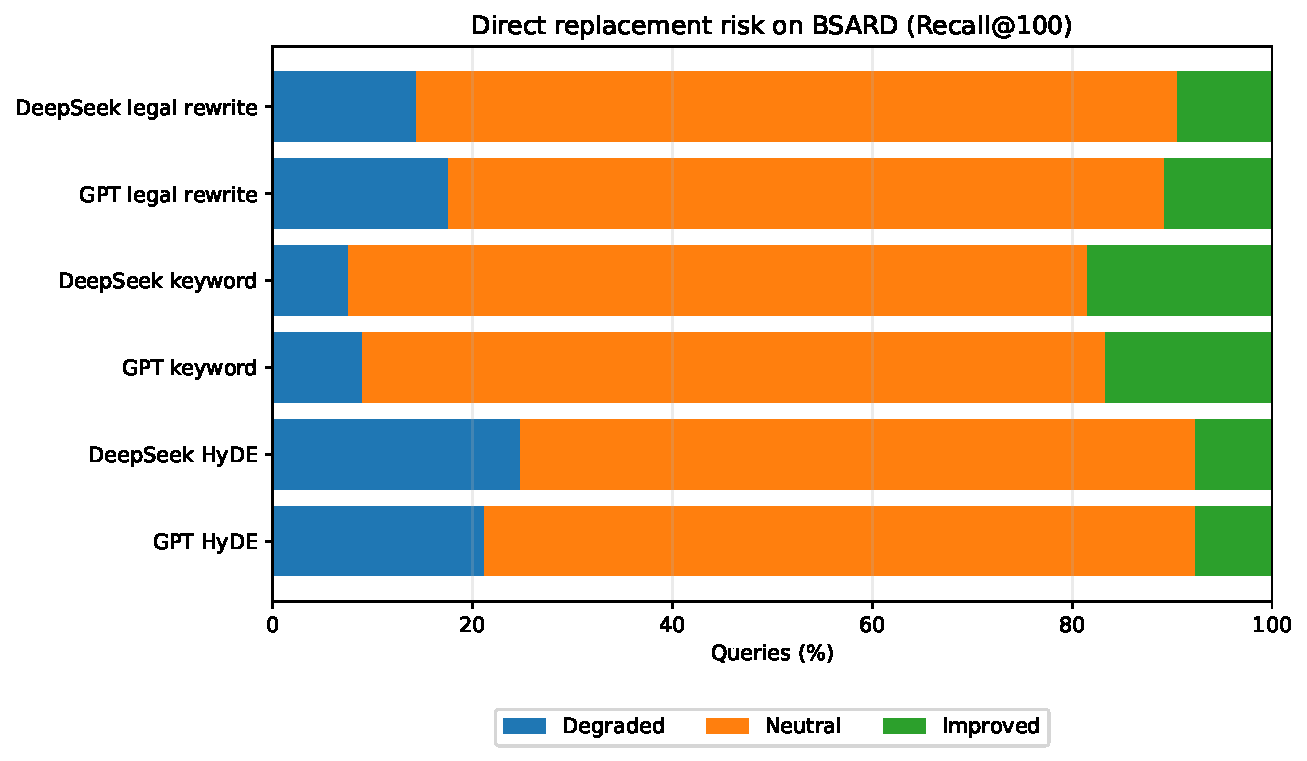
\includegraphics[width=\linewidth]{figs/figure1a_harm_stacked_bsard.pdf}
\textbf{(a) BSARD}
\end{minipage}\hfill
\begin{minipage}[t]{0.49\textwidth}
\centering
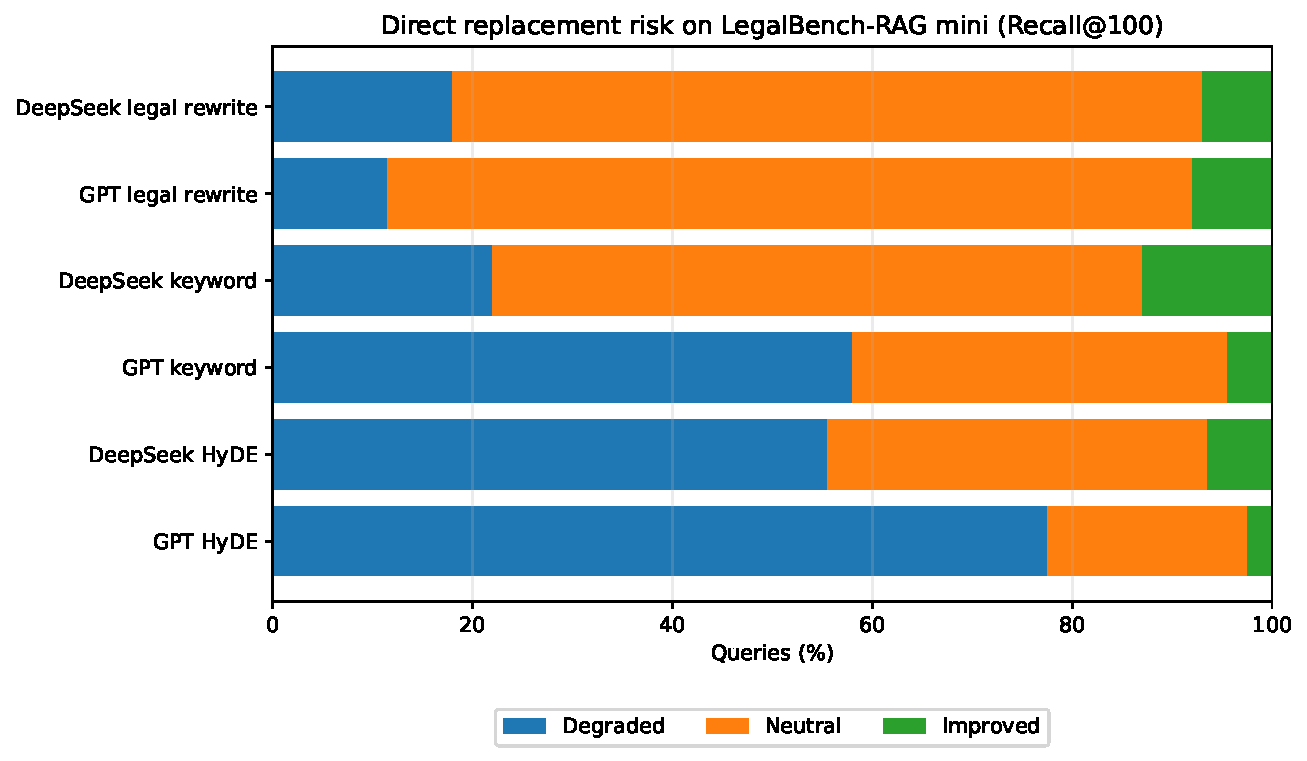
\includegraphics[width=\linewidth]{figs/figure1b_harm_stacked_legalbench.pdf}
\textbf{(b) LegalBench-RAG mini}
\end{minipage}
\caption{Proportion of degraded, neutral and improved queries for
each direct-replacement method, measured on Recall@100. The BSARD
panel includes the two HyDE configurations whose broad-recall
losses remain significant after Holm correction.}
\label{fig:harm-stacked}
\end{figure*}

Figure~\ref{fig:harm-stacked} shows that the two benchmarks
differ in the magnitude and breadth of replacement risk, but not
in the safety conclusion. On BSARD, keyword replacement can
improve broad recall without a robust corrected gain, whereas
both HyDE generators significantly reduce Recall@100. On
LegalBench-RAG mini, GPT keyword and both HyDE variants cause
severe and statistically significant BM25 losses, and the same
harmful pattern persists for the corresponding dense and hybrid
checks. RQ1 is therefore answered negatively: LLM reformulations
should not be used by default as complete substitutes for the
original query. The comparatively stable behaviour of selected
DeepSeek views shows that this conclusion concerns unsafe
replacement, not a universal rejection of reformulation.

\subsection{RQ2 --- Fusion preserving the original query}
\label{sec:results-rq2}

Merging that preserves the original query mitigates the
main risk of direct replacement. On BSARD, the original +
DeepSeek keyword configuration achieves Recall@100 = 0.637,
representing a gain of $+$0.069 after Holm correction, with only
0.45\,\% of queries degraded on Recall@100. The multi-view fusion
of the original + all DeepSeek and GPT reformulations also
significantly improves Recall@100 and MRR@10, but with a higher
harm rate on Recall@100.

The newly completed HyDE comparison makes the protective effect
especially clear. Direct DeepSeek and GPT HyDE replacement changes
BSARD Recall@100 by $-0.112$ and $-0.077$, respectively, whereas
one-view RRF preserving the original query changes it by only
$+0.009$ and $-0.004$. Neither preserving-HyDE change is
significant after Holm correction. Retaining the original query
therefore converts two significant broad-recall losses into
near-zero, non-significant effects.

On LegalBench-RAG mini, the BM25 fusion preserving the original
is particularly effective. The original + DeepSeek keyword
configuration significantly improves Recall@10, MRR@10 and
nDCG@10, while improving Recall@100 on average without reaching
statistical significance after Holm correction. The best
BM25 recall-oriented configuration --- original + DeepSeek
keyword + GPT legal rewrite --- achieves Recall@100 = 0.753,
a gain of $+$0.052, with only 2.00\,\% of queries degraded
on Recall@100 and all four metrics significant after Holm’s
correction. The configuration original + all non-HyDE views
also improves all four metrics significantly.

The preservation pattern also extends to the dense and hybrid
robustness checks. Dense-only RRF yields positive mean Recall@100
gains with low harm rates: $+$0.006 with 4.5\,\% harm for E5
and $+$0.016 with 2.5\,\% harm for BGE in the
original + DeepSeek keyword + GPT legal configuration. These
dense Recall@100 gains are not significant, although the E5
configuration significantly improves nDCG@10. Under hybrid BGE,
the same original-preserving configuration reaches
Recall@100 = 0.788 ($\Delta=+0.054$) with only 1.0\,\% harm
and significant gains in Recall@10, Recall@100 and nDCG@10.
Hybrid E5 also yields positive, low-harm gains, although its
Recall@100 improvement does not reach significance.

\begin{table}[h]
\centering
\caption{Results of the fusion preserving the original
query. The harm rate is reported for Recall@100.
$\dagger$: significant gain after Holm correction.}
\label{tab:fusion}
\resizebox{\columnwidth}{!}{%
\begin{tabular}{llccccc}
\toprule
\textbf{Dataset} &
\textbf{Configuration} &
\textbf{R@10} &
\textbf{R@100} &
\textbf{Harm\,\%} &
\textbf{MRR@10} &
\textbf{nDCG@10} \\
\midrule
BSARD &
Original BM25 &
0.328 &
0.567 &
{--} &
0.268 &
0.248 \\
BSARD &
Original + DeepSeek keyword &
0.331 ($+$0.003){--} &
0.637 ($+$0.069)$\dagger$ &
0.45 &
0.300 ($+$0.032){--} &
0.265 ($+$0.017){--} \\
BSARD &
Original + GPT keyword &
0.331 ($+$0.003){--} &
0.612 ($+$0.045)$\dagger$ &
1.35 &
0.285 ($+$0.017){--} &
0.257 ($+$0.009){--} \\
BSARD &
Original + all (DS+GPT) &
0.345 ($+$0.018){--} &
0.627 ($+$0.059)$\dagger$ &
3.15 &
0.339 ($+$0.071)$\dagger$ &
0.283 ($+$0.035){--} \\
\midrule
LegalBench &
BM25 original &
0.285 &
0.702 &
{--} &
0.213 &
0.193 \\
LegalBench &
Original + DeepSeek keyword &
0.372 ($+$0.088)$\dagger$ &
0.728 ($+$0.027){--} &
7.50 &
0.273 ($+$0.060)$\dagger$ &
0.257 ($+$0.064)$\dagger$ \\
LegalBench &
Original + GPT legal rewrite &
0.322 ($+$0.038){--} &
0.714 ($+$0.013){--} &
3.00 &
0.230 ($+$0.017){--} &
0.219 ($+$0.026)$\dagger$ \\
LegalBench &
Original + DS keyword + GPT legal &
0.369 ($+$0.085)$\dagger$ &
0.753 ($+$0.052)$\dagger$ &
2.00 &
0.265 ($+$0.052)$\dagger$ &
0.255 ($+$0.062)$\dagger$ \\
LegalBench &
Original + all non-HyDE views &
0.367 ($+$0.082)$\dagger$ &
0.743 ($+$0.041)$\dagger$ &
4.00 &
0.287 ($+$0.074)$\dagger$ &
0.264 ($+$0.070)$\dagger$ \\
\bottomrule
\end{tabular}%
}
\end{table}

\begin{figure*}[t]
\centering
\begin{minipage}[t]{0.49\textwidth}
\centering
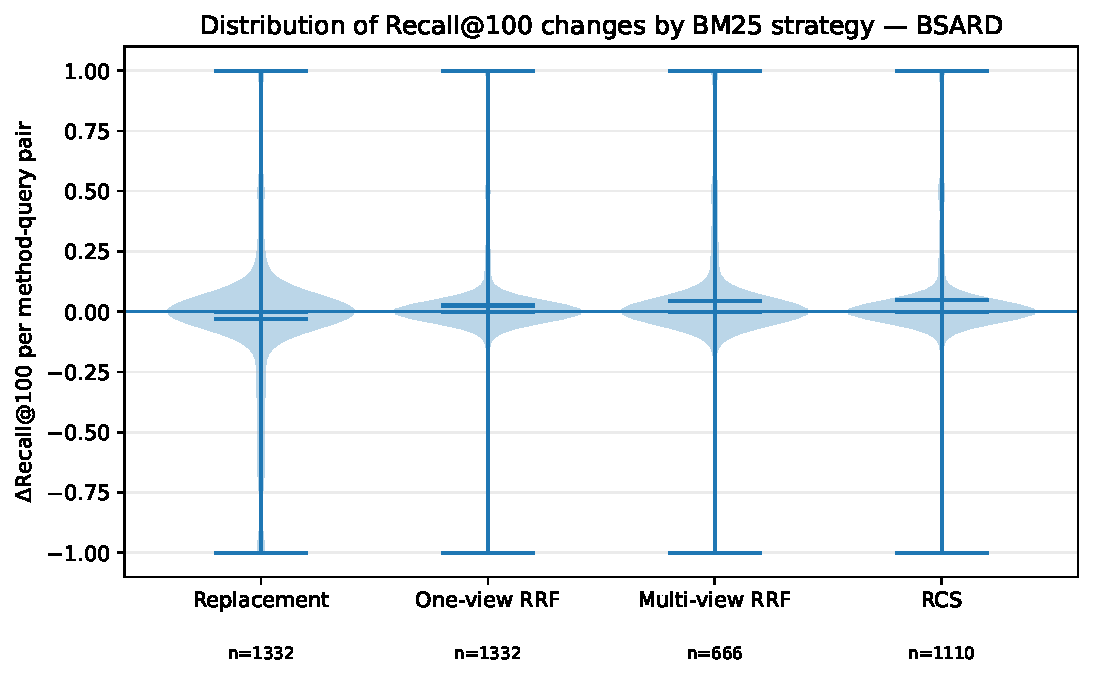
\includegraphics[width=\linewidth]{figs/figure2a_delta_boxplot_bsard.pdf}
\textbf{(a) BSARD}
\end{minipage}\hfill
\begin{minipage}[t]{0.49\textwidth}
\centering
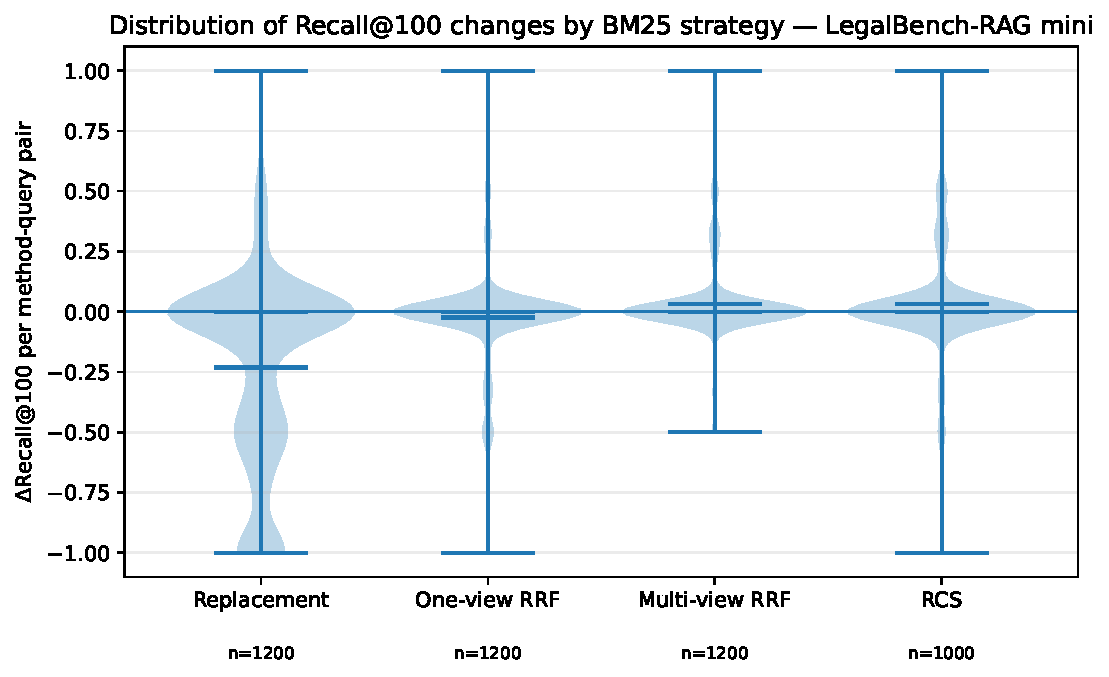
\includegraphics[width=\linewidth]{figs/figure2b_delta_boxplot_legalbench.pdf}
\textbf{(b) LegalBench-RAG mini}
\end{minipage}
\caption{Descriptive distributions of per-query Recall@100 changes
by BM25 strategy. Each violin pools method--query pairs within a
strategy family. The horizontal line indicates no change.
Inferential claims rely on the paired tests reported in the
tables and Appendix~\ref{app:phase1-statistics}, not on the pooled
visual distributions.}
\label{fig:delta-distribution}
\end{figure*}

These results provide a positive answer to RQ2. Preserving
the original query as a retrieval view reduces the risk of
degradation compared with direct replacement while allowing
reformulations to contribute useful vocabulary. This conclusion
is strongest under BM25 and hybrid BGE, where Recall@100 gains
are significant, and remains directionally consistent in
dense-only fusion, where gains are smaller and mostly
non-significant. The central result is not that every
reformulation improves every metric, but that retaining the
original transforms generated views into substantially less
risky auxiliary signals.

\subsection{RQ4 --- RCS and the quality of top-of-list
ranking}
\label{sec:results-rq4}

The Retrieval Consensus Score is used here as a
transparent, non-learning scoring rule to
test whether consensus among reliable views improves the
robustness of top-of-list ranking. It should
not be interpreted as a new
ranking learning method, but as a
diagnostic tool assessing the value of multi-view consensus.

On BSARD, the \textit{All generators strong
consensus} configuration significantly improves Recall@100, MRR@10
and nDCG@10 after Holm correction. The
\textit{DeepSeek top-rank RCS} configuration achieves the best
MRR@10 and nDCG@10 scores on BSARD, suggesting that
consensus improves the quality of the top rankings
when useful views are weighted correctly.

On LegalBench-RAG mini, RCS all non-HyDE achieves the
best top-ranking results:
MRR@10 = 0.336 and nDCG@10 = 0.289, with significant
gains for Recall@10, MRR@10 and nDCG@10. The
gain in Recall@100 is positive but not significant
after Holm correction. The control configuration
including HyDE further improves MRR@10 and nDCG@10
compared to the baseline, but it is less robust than
the non-HyDE configuration and its Recall@100 returns
to practically the baseline level.

\begin{table}[h]
\centering
\caption{RCS results on BSARD and LegalBench-RAG mini.
$\dagger$: significant gain after Holm correction.}
\label{tab:rcs}
\resizebox{\columnwidth}{!}{%
\begin{tabular}{llcccc}
\toprule
\textbf{Dataset} &
\textbf{RCS configuration} &
\textbf{R@10} &
\textbf{R@100} &
\textbf{MRR@10} &
\textbf{nDCG@10} \\
\midrule
BSARD &
Original BM25 &
0.328 &
0.567 &
0.268 &
0.248 \\
BSARD &
DeepSeek top-rank RCS &
0.351 ($+$0.024){--} &
0.600 ($+$0.033)$\dagger$ &
0.346 ($+$0.077)$\dagger$ &
0.289 ($+$0.041)$\dagger$ \\
BSARD &
All generators strong consensus &
0.349 ($+$0.021){--} &
0.622 ($+$0.055)$\dagger$ &
0.339 ($+$0.070)$\dagger$ &
0.285 ($+$0.037)$\dagger$ \\
\midrule
LegalBench &
BM25 original &
0.285 &
0.702 &
0.213 &
0.193 \\
LegalBench &
RCS all non-HyDE &
0.363 ($+$0.079)$\dagger$ &
0.739 ($+$0.037){--} &
0.336 ($+$0.123)$\dagger$ &
0.289 ($+$0.096)$\dagger$ \\
LegalBench &
RCS all views including HyDE &
0.327 ($+$0.043){--} &
0.702 ($+$0.000){--} &
0.305 ($+$0.092)$\dagger$ &
0.261 ($+$0.068)$\dagger$ \\
\bottomrule
\end{tabular}%
}
\end{table}

The comparison between RCS all non-HyDE and RCS all views
including HyDE shows that adding an unreliable view
can dilute the consensus. HyDE does not negate all
top-rank gains when merged with other
views, but it reduces the robustness of the broad recall and
weakens the gains compared to the
non-HyDE configuration. These results provide a positive answer to RQ4:
consensus among reliable views improves the quality of
the top-rank ranking, but this improvement
depends on the selection of views and should not be
interpreted as a general guarantee.

\subsection{RQ5 --- Cross-analysis of the two benchmarks}
\label{sec:results-rq5}

Both benchmarks support the same preservation principle, but
the mechanism and magnitude of reformulation effects differ. On
BSARD, keyword-based reformulations can enrich legal vocabulary
and improve broad recall on average, yet those gains are not
robust after correcting the direct-replacement family. HyDE
replacement is more clearly unsafe: DeepSeek and GPT HyDE
significantly reduce Recall@100 by 0.112 and 0.077. Preserving
the original query reduces the corresponding changes to
$+0.009$ and $-0.004$, while original + DeepSeek keyword
produces a significant Recall@100 gain with a 0.45\,\% harm rate.

On LegalBench-RAG mini, the risk is more strongly tied to source
identity. Many contracts and policies contain similar language
but are distinguished by party names, application names or file
paths. GPT keyword and HyDE replacement produce severe losses
under BM25 and remain significantly harmful under E5, BGE and
the tested hybrids. This persistence shows that semantic
retrieval does not automatically compensate for a reformulation
that loses or dilutes source-specific information. At the same
time, selected DeepSeek views remain substantially more stable,
confirming that reformulation quality matters.

Original-preserving fusion generalises in a differentiated way.
It produces significant Recall@100 gains under BM25 and hybrid
BGE, while dense-only RRF yields small positive mean Recall@100
gains with low harm rates but no significant recall improvement.
RCS remains the strongest top-rank consensus diagnostic in the
BM25 experiments. Figure~\ref{fig:grouped-bar} summarises these
representative strategies across the four retrieval metrics.

\begin{table}[t]
\centering
\caption{Cross-dataset and cross-retriever summary of key
results and design implications.}
\label{tab:cross-dataset}
\resizebox{\columnwidth}{!}{%
\begin{tabular}{p{2.8cm}p{3.9cm}p{4.6cm}p{3.4cm}}
\toprule
\textbf{Observation} &
\textbf{BSARD evidence} &
\textbf{LegalBench evidence} &
\textbf{Implication} \\
\midrule
Preserving fusion &
BM25 original + DS kw.:
$\Delta$R@100 = $+$0.069$\dagger$,
harm 0.45\% &
BM25: $+$0.052$\dagger$, harm 2\%;
hybrid BGE: $+$0.054$\dagger$, harm 1\% &
Preserve the original query \\
\midrule
Risky replacement &
Keyword gains are non-significant;
DS/GPT HyDE reduce R@100 by
0.112/0.077$\downarrow$ &
GPT kw. and both HyDE variants are significantly harmful
under BM25; harmful replacement persists under E5, BGE and
hybrid retrieval &
Do not treat reformulations as safe substitutes \\
\midrule
Dense-only preservation &
Not evaluated on BSARD &
Positive mean R@100 gains with 2.5--4.5\% harm;
R@100 gains non-significant &
Preservation stabilises dense retrieval but gains are modest \\
\midrule
Useful consensus &
RCS$\dagger$ on R@100, MRR@10 and nDCG@10 &
Non-HyDE RCS$\dagger$ on R@10, MRR@10 and nDCG@10 &
Select reliable views \\
\midrule
HyDE sensitivity &
Significant R@100 replacement losses;
preserving RRF changes them to $+0.009$ and $-0.004$ &
Severe replacement losses persist across tested retrievers
and remain in the BM25 chunk-only ablation &
Validate pseudo-passage views and preserve the original \\
\bottomrule
\end{tabular}%
}
\end{table}

\begin{figure*}[t]
\centering
\begin{minipage}[t]{0.49\textwidth}
\centering
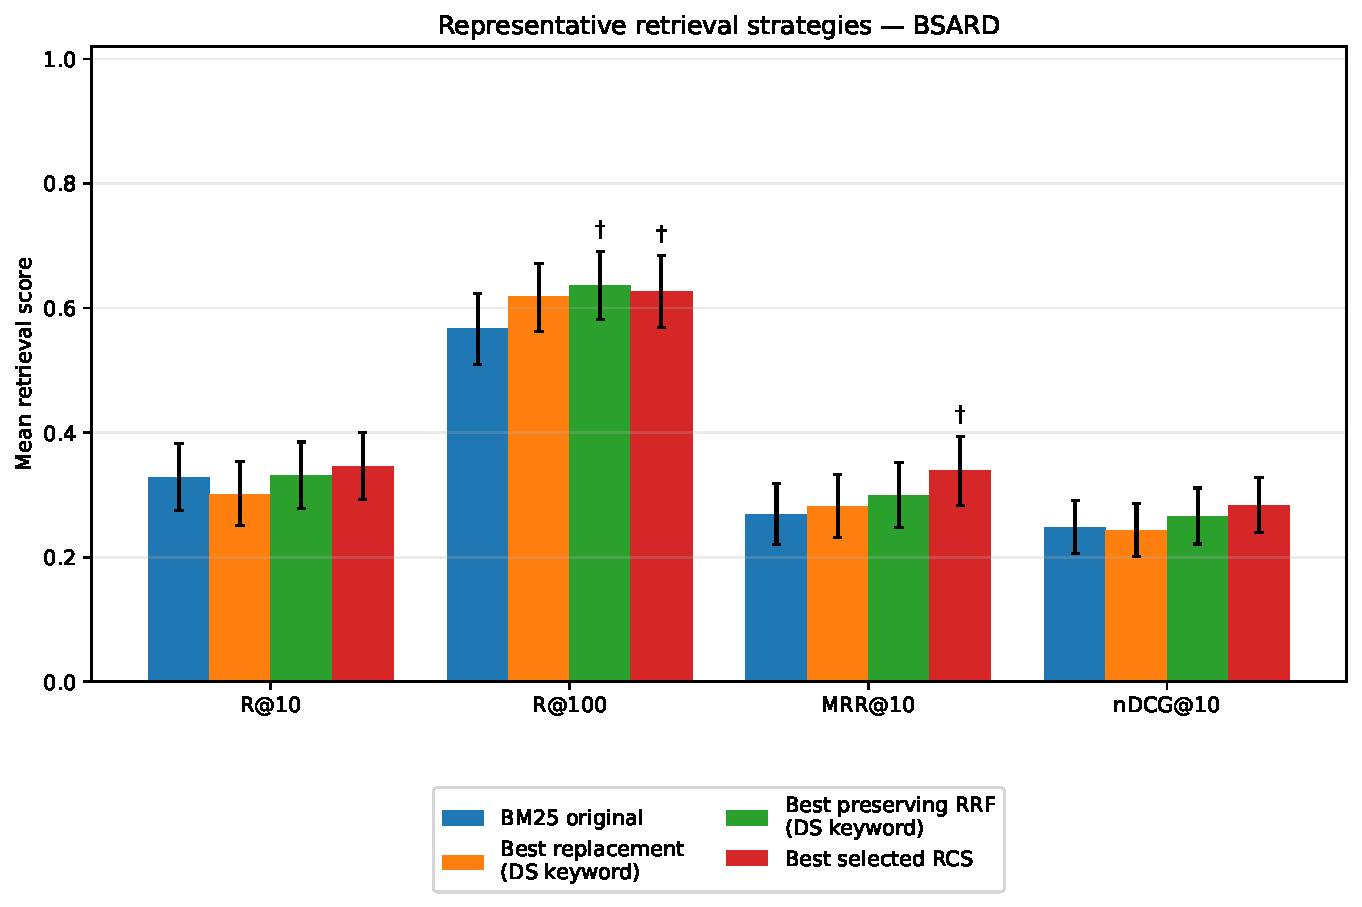
\includegraphics[width=\linewidth]{figs/figure3a_grouped_metrics_bsard.pdf}
\textbf{(a) BSARD}
\end{minipage}\hfill
\begin{minipage}[t]{0.49\textwidth}
\centering
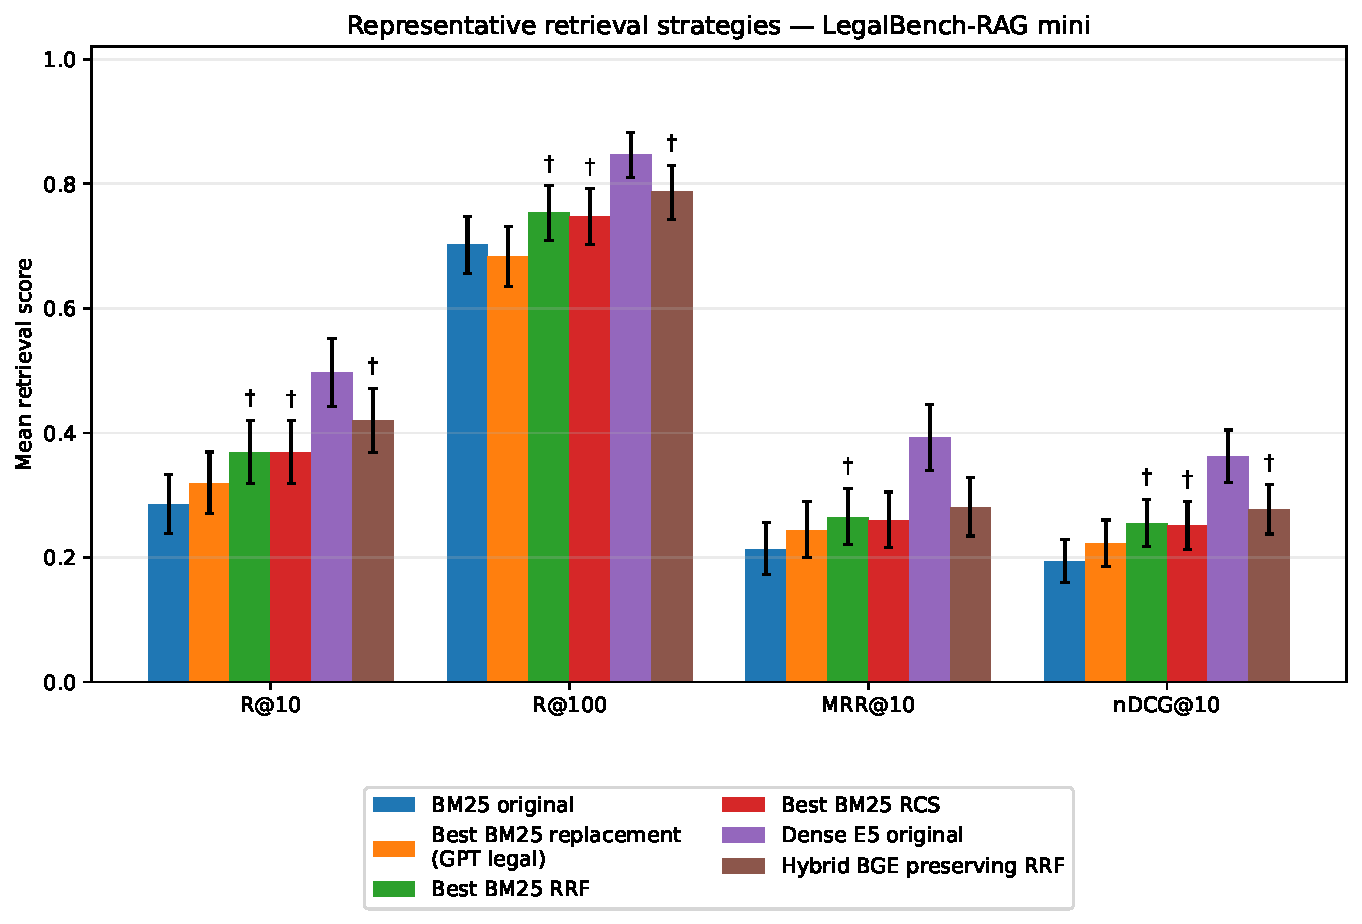
\includegraphics[width=\linewidth]{figs/figure3b_grouped_metrics_legalbench.pdf}
\textbf{(b) LegalBench-RAG mini}
\end{minipage}
\caption{Comparison of representative retrieval strategies across
the four metrics. Strategies were fixed using Recall@100 before
plotting all metrics. Error bars show 95\% bootstrap confidence
intervals; $\dagger$ and $\downarrow$ denote significant positive
and negative candidate--baseline differences after Holm correction.}
\label{fig:grouped-bar}
\end{figure*}

The overarching conclusion is not that any single model or
reformulation type is universally superior. The central finding
is a design principle: in source-sensitive legal tasks, it is
safer to preserve the original query as the retrieval anchor and
treat LLM reformulations as auxiliary views. RQ5 is therefore
answered positively across the two retrieval profiles and, on
LegalBench-RAG mini, across the tested lexical, dense and hybrid
families. The remaining scope restriction is that dense and
hybrid experiments use two encoders, the filepath+chunk
representation and a single fixed hybrid weight.

\subsection{Dense and hybrid baselines}
\label{sec:dense-baselines}

The dense and hybrid robustness checks confirm that harmful
replacement is not specific to BM25 in the canonical
filepath+chunk setting. The original-query dense baselines are
strong in absolute terms: E5 reaches Recall@100 = 0.847 and BGE
reaches 0.818, compared with 0.702 for the BM25 original-query
baseline. Nevertheless, GPT keyword replacement reduces
Recall@100 to 0.368 with E5 and 0.380 with BGE, while GPT HyDE
falls to 0.096 and 0.137, respectively. These four replacement
configurations are significantly worse than their corresponding
dense original-query baselines on all metrics. DeepSeek HyDE is
also significantly harmful under both dense encoders, with
$\Delta$Recall@100 = $-0.428$ for E5 and $-0.369$ for BGE.

These results do not imply that all dense reformulations are
harmful. DeepSeek keyword is comparatively stable: with E5 it
improves all four mean metrics, including Recall@100 by 0.004,
and yields a marginal Holm-corrected improvement in MRR@10
($\Delta=+0.071$, $p_{\mathrm{Holm}}=0.0496$). Because this
result lies close to the significance threshold, we treat it as
a supportive rather than central effect. The contrast between
stable DeepSeek views and harmful GPT keyword or HyDE views shows
that performance depends on the content and specificity of the
reformulation, not only on the retriever family.

\begin{table*}[t]
\centering
\caption{Dense retrieval results on LegalBench-RAG mini using
filepath+chunk indexing. Harm is reported for Recall@100.
$\dagger$: significant positive gain; $\downarrow$: significant
degradation; {--}: non-significant after Holm correction.}
\label{tab:dense-results}
\resizebox{\textwidth}{!}{%
\begin{tabular}{llccccc}
\toprule
\textbf{Model} &
\textbf{Query configuration} &
\textbf{R@10} &
\textbf{R@100} &
\textbf{Harm\,\%} &
\textbf{MRR@10} &
\textbf{nDCG@10} \\
\midrule
E5 & Original &
0.497 & 0.847 & {--} & 0.392 & 0.362 \\
E5 & DeepSeek keyword replacement &
0.532 ($+$0.036){--} &
0.852 ($+$0.004){--} &
8.5 &
0.463 ($+$0.071)$\dagger$ &
0.407 ($+$0.046){--} \\
E5 & DeepSeek HyDE replacement &
0.224 ($-$0.272)$\downarrow$ &
0.419 ($-$0.428)$\downarrow$ &
55.0 &
0.207 ($-$0.185)$\downarrow$ &
0.172 ($-$0.189)$\downarrow$ \\
E5 & GPT keyword replacement &
0.167 ($-$0.329)$\downarrow$ &
0.368 ($-$0.480)$\downarrow$ &
63.0 &
0.160 ($-$0.232)$\downarrow$ &
0.134 ($-$0.228)$\downarrow$ \\
E5 & GPT HyDE replacement &
0.033 ($-$0.464)$\downarrow$ &
0.096 ($-$0.751)$\downarrow$ &
89.0 &
0.028 ($-$0.364)$\downarrow$ &
0.022 ($-$0.339)$\downarrow$ \\
E5 & RRF: original + DS kw. + GPT legal &
0.519 ($+$0.022){--} &
0.853 ($+$0.006){--} &
4.5 &
0.424 ($+$0.032){--} &
0.389 ($+$0.027)$\dagger$ \\
\midrule
BGE & Original &
0.441 & 0.818 & {--} & 0.372 & 0.341 \\
BGE & DeepSeek keyword replacement &
0.469 ($+$0.027){--} &
0.785 ($-$0.033){--} &
13.5 &
0.400 ($+$0.028){--} &
0.362 ($+$0.021){--} \\
BGE & DeepSeek HyDE replacement &
0.249 ($-$0.192)$\downarrow$ &
0.449 ($-$0.369)$\downarrow$ &
50.5 &
0.217 ($-$0.155)$\downarrow$ &
0.190 ($-$0.151)$\downarrow$ \\
BGE & GPT keyword replacement &
0.191 ($-$0.250)$\downarrow$ &
0.380 ($-$0.438)$\downarrow$ &
60.5 &
0.163 ($-$0.209)$\downarrow$ &
0.150 ($-$0.191)$\downarrow$ \\
BGE & GPT HyDE replacement &
0.038 ($-$0.403)$\downarrow$ &
0.137 ($-$0.681)$\downarrow$ &
87.0 &
0.034 ($-$0.339)$\downarrow$ &
0.029 ($-$0.312)$\downarrow$ \\
BGE & RRF: original + DS kw. + GPT legal &
0.467 ($+$0.026){--} &
0.834 ($+$0.016){--} &
2.5 &
0.394 ($+$0.021){--} &
0.359 ($+$0.018){--} \\
\bottomrule
\end{tabular}%
}
\end{table*}

Original-preserving dense RRF stabilises the ranking but yields
modest gains relative to already strong dense baselines. For E5,
original + DeepSeek keyword + GPT legal rewrite improves
Recall@100 by 0.006 with 4.5\,\% harm and significantly improves
nDCG@10. For BGE, the same fusion improves all four mean metrics,
including Recall@100 by 0.016 with 2.5\,\% harm, but none reaches
significance after Holm correction. The all-non-HyDE dense
fusions show the same qualitative pattern: positive but
non-significant Recall@100 gains and low harm rates.

Hybrid replacement remains vulnerable. With the fixed
$\lambda=0.5$ score combination, GPT keyword and GPT HyDE are
significantly harmful on all four metrics for both E5 and BGE
hybrids. DeepSeek HyDE is also strongly harmful, although its
MRR@10 loss with hybrid E5 does not reach significance. In
contrast, original-preserving hybrid RRF produces the strongest
recall-oriented fusion result on LegalBench-RAG mini. With BGE,
original + DeepSeek keyword + GPT legal rewrite reaches
Recall@100 = 0.788, a gain of 0.054 with only 1.0\,\% harm, and
significantly improves Recall@10, Recall@100 and nDCG@10.

\begin{table*}[t]
\centering
\caption{Hybrid BM25+dense results on LegalBench-RAG mini with
$\lambda=0.5$ and filepath+chunk indexing. Harm is reported for
Recall@100.}
\label{tab:hybrid-results}
\resizebox{\textwidth}{!}{%
\begin{tabular}{llccccc}
\toprule
\textbf{Dense model} &
\textbf{Query configuration} &
\textbf{R@10} &
\textbf{R@100} &
\textbf{Harm\,\%} &
\textbf{MRR@10} &
\textbf{nDCG@10} \\
\midrule
E5 & Original &
0.286 & 0.732 & {--} & 0.213 & 0.197 \\
E5 & DeepSeek HyDE replacement &
0.140 ($-$0.147)$\downarrow$ &
0.377 ($-$0.355)$\downarrow$ &
52.0 &
0.139 ($-$0.075){--} &
0.106 ($-$0.090)$\downarrow$ \\
E5 & GPT keyword replacement &
0.115 ($-$0.171)$\downarrow$ &
0.337 ($-$0.395)$\downarrow$ &
57.5 &
0.106 ($-$0.107)$\downarrow$ &
0.089 ($-$0.108)$\downarrow$ \\
E5 & GPT HyDE replacement &
0.035 ($-$0.251)$\downarrow$ &
0.142 ($-$0.590)$\downarrow$ &
76.5 &
0.030 ($-$0.184)$\downarrow$ &
0.024 ($-$0.172)$\downarrow$ \\
E5 & RRF: original + DS kw. + GPT legal &
0.350 ($+$0.063)$\dagger$ &
0.769 ($+$0.037){--} &
2.5 &
0.247 ($+$0.033){--} &
0.236 ($+$0.040)$\dagger$ \\
E5 & RRF: original + all non-HyDE &
0.368 ($+$0.082)$\dagger$ &
0.768 ($+$0.037){--} &
4.0 &
0.245 ($+$0.031){--} &
0.240 ($+$0.044)$\dagger$ \\
\midrule
BGE & Original &
0.352 & 0.734 & {--} & 0.248 & 0.235 \\
BGE & DeepSeek HyDE replacement &
0.182 ($-$0.171)$\downarrow$ &
0.416 ($-$0.319)$\downarrow$ &
49.5 &
0.153 ($-$0.096)$\downarrow$ &
0.132 ($-$0.103)$\downarrow$ \\
BGE & GPT keyword replacement &
0.138 ($-$0.215)$\downarrow$ &
0.361 ($-$0.374)$\downarrow$ &
57.5 &
0.121 ($-$0.128)$\downarrow$ &
0.104 ($-$0.131)$\downarrow$ \\
BGE & GPT HyDE replacement &
0.048 ($-$0.304)$\downarrow$ &
0.184 ($-$0.551)$\downarrow$ &
76.0 &
0.055 ($-$0.193)$\downarrow$ &
0.038 ($-$0.196)$\downarrow$ \\
BGE & RRF: original + DS kw. + GPT legal &
0.420 ($+$0.067)$\dagger$ &
0.788 ($+$0.054)$\dagger$ &
1.0 &
0.281 ($+$0.033){--} &
0.277 ($+$0.042)$\dagger$ \\
BGE & RRF: original + all non-HyDE &
0.426 ($+$0.073)$\dagger$ &
0.774 ($+$0.040)$\dagger$ &
3.0 &
0.293 ($+$0.045){--} &
0.285 ($+$0.050)$\dagger$ \\
\bottomrule
\end{tabular}%
}
\end{table*}

The hybrid results should not be interpreted as showing that a
fixed 50--50 hybrid is superior to dense retrieval. The original
E5 and BGE dense runs remain stronger in absolute terms than the
corresponding hybrid baselines. Instead, the hybrid experiment
tests whether the replacement-versus-preservation pattern
survives score-level lexical/semantic combination. It does:
unsafe replacement remains strongly harmful, whereas
original-preserving RRF provides low-harm gains, reaching
significant broad-recall improvement with BGE.

\section{Analysis of anchor loss (RQ3)}
\label{sec:anchor-loss}

This section addresses RQ3: does anchor loss contribute to the
severe performance degradation observed during direct replacement in
document-centric legal retrieval? We answer this question through a
diagnostic analysis based on a manually audited conservative lexical
anchor-preservation proxy, not through a complete APR gold standard.
The proxy retains observable source cues that occur in the original
query: tokens overlapping the resolved source path and tokens parsed
from named parties, organisations, applications or products. Its
construction and validation are reported in
Section~\ref{sec:anchor-extraction}.

The diagnostic identifies a recurring pattern: certain reformulations
retain the broad legal theme of the query but remove the identifiers
that distinguish the intended source. This removal is particularly
detrimental in LegalBench-RAG mini, where several documents may contain
legally similar clauses but belong to different contracts, policies or
transactions.

The dense and hybrid experiments broaden the interpretation of
this pattern. GPT keyword and both HyDE-style replacements remain
strongly harmful under E5, BGE and the tested hybrids, even though
these retrievers do not depend exclusively on exact lexical
matching. This evidence is consistent with a wider
\textit{source-dilution} mechanism: a reformulation can become semantically plausible for many
documents of the same class while losing the information that
identifies the correct one. The dense results therefore strengthen
the diagnosis, but they do not prove that every degradation is
caused exclusively by lexical anchor omission.

\subsection{Lexical preservation of anchors by model
and by task}
\label{sec:apr-by-model}

The anchor preservation diagnosis shows that
the collapse of certain reformulations on
LegalBench-RAG mini is not due to a
parsing error or a JSON format issue. It corresponds
to a genuine change in the lexical content of the
query. In particular, GPT keyword reformulations
tend to remove part names,
document identifiers or source indices that
are useful for BM25 in a
document-centric indexing approach.


The clearest example is found in contractual
tasks. On ContractNLI, GPT keyword shows
an average retention rate of almost zero for anchor tokens,
with a very high proportion of zero retention. This loss
coincides with a significant deterioration in
retrieval metrics. On MAUD, the contrast is even more
clear: GPT keyword removes virtually all the
anchors tracked by our diagnostic, whilst
DeepSeek keyword and GPT legal rewrite preserve
identifiers much more effectively, which corresponds to
better retrieval results.

\begin{table}[h]
\centering
\caption{Examples from the final conservative anchor-preservation
proxy on LegalBench-RAG mini. Retention values are means within the
specified task and reformulation condition; retrieval columns report
mean deltas relative to the original-query BM25 baseline.}
\label{tab:anchor-retention-diagnostic}
\resizebox{\columnwidth}{!}{%
\begin{tabular}{llcccc}
\toprule
\textbf{Task} &
\textbf{Rephrasing} &
\textbf{Average retention} &
\textbf{Zero retention} &
\textbf{$\Delta$R@100} &
\textbf{$\Delta$nDCG@10} \\
\midrule
ContractNLI &
GPT keyword &
0.015 &
0.96 &
$-$0.423 &
$-$0.326 \\
MAUD &
GPT keyword &
0.000 &
1.00 &
$-$0.483 &
$-$0.082 \\
MAUD &
DeepSeek keyword &
0.957 &
0.00 &
$+$0.035 &
$+$0.098 \\
MAUD &
GPT legal rewrite &
1.000 &
0.00 &
$-$0.011 &
$+$0.030 \\
\bottomrule
\end{tabular}%
}
\end{table}

This descriptive table is not an exhaustive APR benchmark. It is
consistent with the audited and query-clustered analysis in
Section~\ref{sec:apr-correlation}: configurations that retain few
observable source cues tend to produce larger losses in broad coverage,
whereas DeepSeek keyword and GPT legal rewrite on MAUD preserve nearly
all tracked cues and remain substantially more stable. The association
is probabilistic rather than deterministic, and retained anchors do not
guarantee that every added term is useful.

\subsection{Manually audited lexical anchor-preservation proxy}
\label{sec:apr-correlation}

We quantify anchor preservation with a conservative lexical proxy rather
than claiming a complete manually annotated APR benchmark. For each
LegalBench-RAG mini query, the proxy retains two kinds of source-identifying
tokens that are present in the original query: tokens overlapping the
resolved source path and tokens parsed from named parties, organisations,
applications or products. The score is the fraction of these extracted
tokens retained by the reformulation.

The extractor was audited on a deterministic, task-stratified sample of
40 unique queries, with ten queries from each task. Under a strict manual
annotation that includes every non-function component of a compound
party or application name, the proxy exactly matched 16 of the 40
queries. At token level, it recovered 100 of 149 manually identified
tokens (recall 0.671) and introduced no spurious tokens in the reviewed
sample (descriptive precision 1.000; F1 0.803). Most omissions were
corporate suffixes or generic components embedded in compound names,
such as \textit{Corporation}, \textit{Services} or \textit{Messenger}.
The audit therefore characterises the measure as a high-precision,
conservative proxy for source-identifying content, not as an exhaustive
APR annotation.

To avoid pseudo-replication, the inferential analysis treats the 200
queries as clusters while preserving their six reformulation rows.
The association is estimated after ranking and centring both variables
within generator $\times$ reformulation-type $\times$ task strata.
Confidence intervals use query-cluster bootstrap with 10,000 iterations;
$p$-values use query-cluster permutation with 10,000 iterations and are
Holm-corrected across the 12 pooled proxy--metric tests.

\begin{table}[t]
\centering
\caption{Query-clustered association between anchor-preservation proxies
and $\Delta$Recall@100 on LegalBench-RAG mini. Correlations are computed
after ranking and centring within generator $\times$ reformulation type
$\times$ task strata. Confidence intervals use query-cluster bootstrap;
$p$-values use query-cluster permutation and Holm correction across the
12 pooled proxy--metric tests.}
\label{tab:anchor-proxy-correlation}
\begin{tabular}{lccc}
\toprule
Proxy & $\rho$ & 95\% CI & $p_{\mathrm{Holm}}$ \\
\midrule
Combined & 0.179 & [0.116, 0.242] & 0.0012 \\
File-path overlap & 0.197 & [0.123, 0.268] & 0.0012 \\
Entity/name & 0.191 & [0.134, 0.249] & 0.0012 \\
\bottomrule
\end{tabular}
\end{table}


The combined proxy is positively associated with
$\Delta$Recall@100 ($\rho=0.179$, 95\% cluster-bootstrap
CI $[0.116,0.242]$, $p_{\mathrm{Holm}}=0.0012$).
The file-path and entity/name components show similar associations
($\rho=0.197$ and $\rho=0.191$, respectively; both
$p_{\mathrm{Holm}}=0.0012$). No pooled association survives Holm
correction for Recall@10, MRR@10 or nDCG@10. The observed mechanism
therefore concerns broad retrieval coverage more clearly than immediate
top-rank quality.

\begin{figure*}[t]
\centering
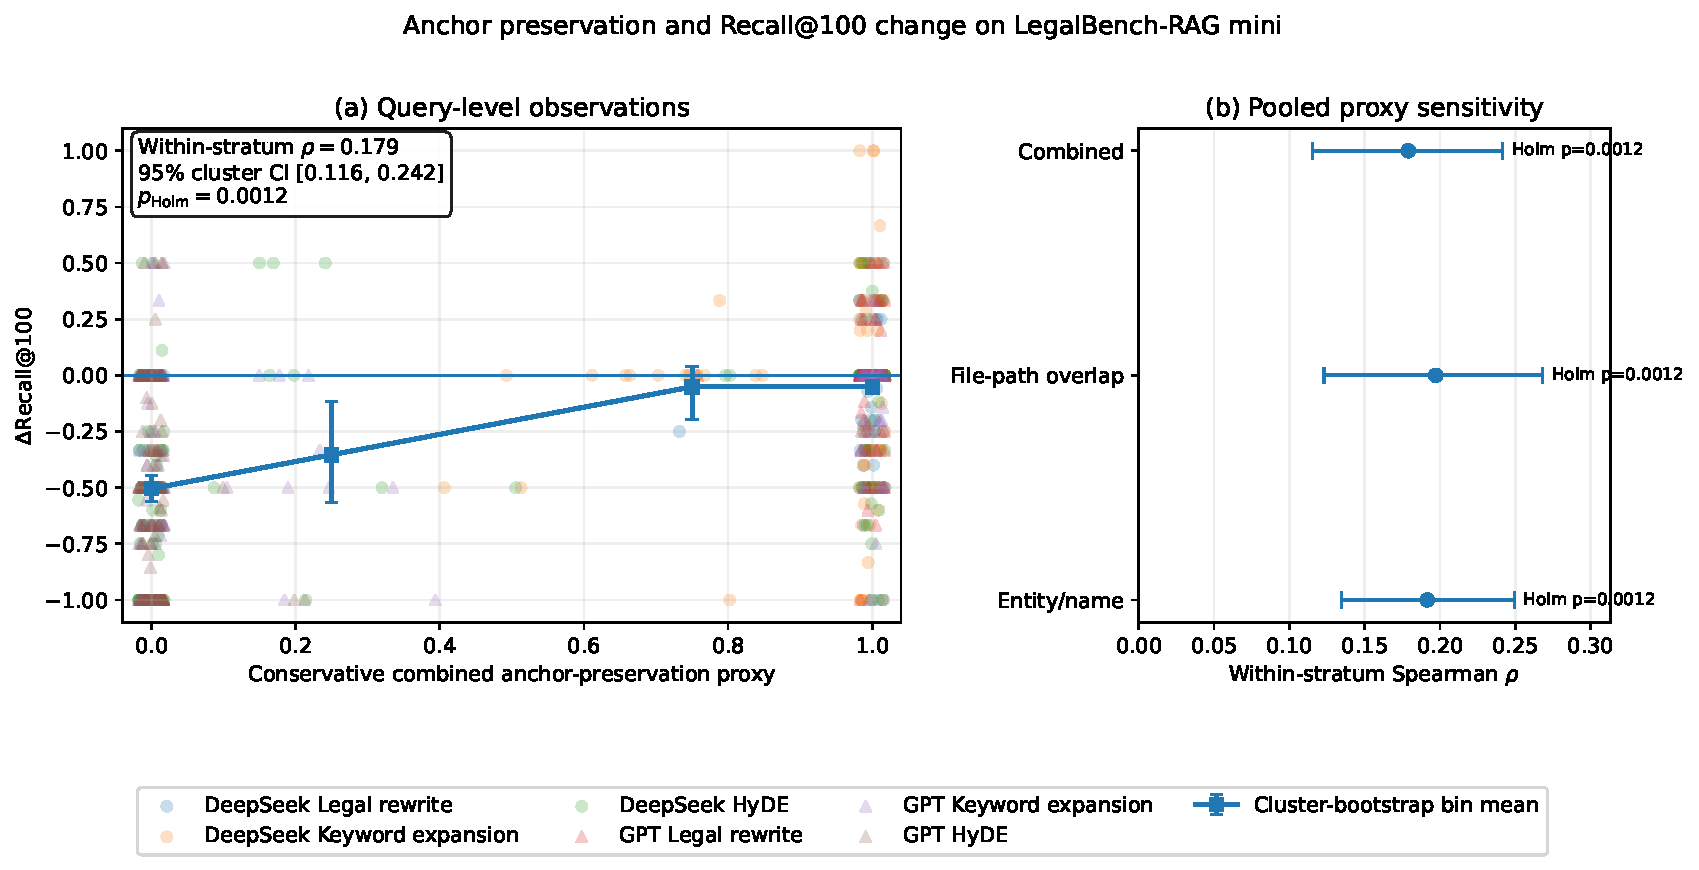
\includegraphics[width=0.95\textwidth]{figs/figure4_anchor_preservation_final.pdf}
\caption{Relationship between the manually audited conservative lexical
anchor-preservation proxy and $\Delta$Recall@100 under direct replacement
on LegalBench-RAG mini. Panel (a) uses deterministic horizontal jitter to
display repeated proxy values; squares show query-cluster-bootstrap means
within four retention ranges. Panel (b) reports pooled within-stratum
correlations for the combined, file-path and entity/name proxy definitions.
The association is diagnostic and does not establish that anchor loss is
the sole causal mechanism of every retrieval degradation.}
\label{fig:apr-scatter}
\end{figure*}

The task- and reformulation-specific analysis is more heterogeneous.
After Holm correction across 24 subgroup tests, only DeepSeek HyDE on
CUAD remains significant ($\rho=0.467$, 95\% bootstrap
CI $[0.213,0.678]$, $p_{\mathrm{Holm}}=0.0176$). Positive but
non-significant trends also appear for DeepSeek HyDE on MAUD and
PrivacyQA. These subgroup results are therefore treated as exploratory.

Taken together, the manually audited proxy and the retriever robustness
experiments support a positive but bounded answer to RQ3. Better
preservation of observable source-identifying content is associated with
smaller Recall@100 losses, and reformulations with near-zero retention
are among the most harmful. However, the modest pooled effect size and
the conservative, incomplete token coverage show that anchor loss is one
important component of a broader source-dilution process, not an exhaustive
causal explanation.

\subsection{Qualitative coding framework for degraded queries}
\label{sec:taxonomy}

Inspection of strongly degraded GPT keyword and GPT HyDE cases suggests
seven recurring mechanisms that can guide future document-level source
audits:
\begin{enumerate}
    \item \textbf{Loss of party names}: the reformulation removes the
    names of the contracting parties, weakening identification of the
    target contract.
    \item \textbf{Loss of application or service names}: the product,
    service or application named in the query disappears.
    \item \textbf{Loss of document identifier}: a title, file-path cue,
    transaction reference or other specific identifier is removed.
    \item \textbf{HyDE pseudo-passage too generic}: the hypothetical
    passage remains legally plausible but contains no identifier
    traceable to the intended source.
    \item \textbf{Excessive abstraction}: specific facts are replaced by
    generic legal concepts.
    \item \textbf{Good topic, potential wrong-source risk}: the
    reformulation is thematically appropriate for a document class but
    no longer distinguishes the intended member of that class.
    \item \textbf{Lexical dilution}: numerous generated terms reduce the
    relative contribution of the few source cues that remain.
\end{enumerate}

These categories are reported as a qualitative coding framework, not as
a frequency distribution. A horizontal frequency chart is deliberately
omitted because the full set of harmed cases was not independently coded
and no inter-annotator agreement was measured. This preserves the
mechanistic observations without presenting unvalidated category counts
as quantitative evidence.

\subsection{Illustrative source-sensitivity cases}
\label{sec:qualitative-cases}

Table~\ref{tab:wrong-source} preserves three illustrative cases used to
explain the anchor-loss mechanism. The table analyses the query,
reformulation and expected source identity; it does not claim that a
specific alternative retrieved document has been manually verified.
Direct document-level source attribution is reserved for future work.

\begin{table*}[t]
\centering
\caption{Illustrative source-sensitivity cases under LLM query
replacement. These examples diagnose anchor behaviour and source-confusion
risk; they are not presented as manually verified wrong-document
retrieval events.}
\label{tab:wrong-source}
\small
\begin{tabular}{p{3.0cm}p{3.7cm}p{2.5cm}p{2.5cm}p{4.0cm}}
\toprule
\textbf{Original query} &
\textbf{Reformulation} &
\textbf{Anchor behaviour} &
\textbf{Expected source} &
\textbf{Diagnostic interpretation} \\
\midrule
NDA between DoiT and ICN; question on independent development
&
independent development, independently developed information,
similar information, Confidential Information, Receiving Party,
NDA exceptions
&
DoiT and ICN removed
&
NDA DoiT--ICN
&
The legal topic is preserved, but the party names needed to
distinguish the intended NDA are removed, creating a clear
source-confusion risk. \\
\midrule
Fiverr privacy policy; question regarding the visibility of information
&
posted jobs visibility, job postings, public profile,
Fiverr privacy policy
&
Fiverr retained
&
Fiverr policy
&
The application anchor remains present. This counterexample shows
that reformulation is not harmful merely because it adds topical terms;
retaining the source cue can limit source dilution. \\
\midrule
MAUD acquisition agreement involving The Michaels Companies and Apollo
&
closing condition, compliance with covenants, acquisition agreement,
material obligations
&
Party names and transaction identifiers removed
&
Michaels--Apollo agreement
&
The reformulation becomes generic to many acquisition agreements.
Without the transaction parties, a semantically similar clause from
another transaction could be favoured. \\
\bottomrule
\end{tabular}
\end{table*}

These cases clarify the distinction between thematic relevance and
source accuracy. A reformulation may remain legally coherent while
removing the information required to attribute evidence to the intended
document. Because the actually retrieved alternative sources were not
manually adjudicated in this study, the table supports a mechanism-level
interpretation rather than a document-level error-rate claim.

\subsection{Summary of RQ3}

The results provide a positive but bounded answer to RQ3. The manually
audited conservative lexical proxy shows that better preservation of
observable source-identifying content is associated with smaller
Recall@100 losses under direct replacement. The pooled within-stratum
association is modest but statistically robust
($\rho=0.179$, 95\% cluster-bootstrap CI $[0.116,0.242]$,
$p_{\mathrm{Holm}}=0.0012$), and the path-overlap and entity/name
components yield similar results. No pooled association survives
correction for Recall@10, MRR@10 or nDCG@10, indicating that the
diagnostic is most clearly linked to broad retrieval coverage.

The task summaries are consistent with this result. GPT keyword and GPT
HyDE often retain almost none of the tracked source cues on
ContractNLI, CUAD and MAUD and produce the largest Recall@100 losses.
DeepSeek keyword and GPT legal rewrite preserve substantially more cues
and are generally more stable. The only subgroup association surviving
Holm correction is DeepSeek HyDE on CUAD; the remaining subgroup
patterns are exploratory.

The dense and hybrid robustness checks further show that the harmful
pattern is not confined to exact lexical matching. GPT keyword and both
HyDE-style replacements remain strongly harmful under E5, BGE and the
tested hybrids, which is consistent with a broader
\textit{source-dilution} mechanism. Conversely, original-preserving
fusion remains low-risk across BM25, dense and hybrid settings.

The manual audit also defines the limits of the claim. The proxy is
high-precision but incomplete under a strict full-name annotation, and
the correlation does not prove that anchor loss is the sole cause of
every degradation. The evidence therefore supports anchor loss as an
important and measurable component of source dilution in
document-centric legal retrieval, not as an exhaustive causal account.

\section{Robustness and ablation studies}
\label{sec:robustness}
This section documents the robustness analyses completed in the
present study and explicitly delimits comparisons that were not included.
The distinction is important: unavailable counterfactual matrices or
hyperparameter sweeps are treated as scope limitations, not as pending
results embedded in the submitted evidence.

\subsection{RRF with versus without the original query}
\label{sec:ablation-original}
\paragraph{Motivation.}
The central principle of this paper is that the
original query must remain a retrieval view. This
ablation therefore assesses whether adding the original query
to the merge reduces the negative effects observed
when the reformulations entirely replace the
user query. It compares direct replacement,
where only the reformulation is used, with
original-preserving RRF merge, where the original query
remains present as a retrieval view.
\paragraph{Coverage in this study.}
The matched single-reformulation comparison is fully covered:
direct replacement uses only $\hat{q}$, whereas one-view RRF merges
$q$ and the same $\hat{q}$. This provides a controlled
with-versus-without-original comparison for the four reported
reformulation conditions. A separate counterfactual matrix removing
$q$ from every multi-view fusion was not evaluated; conclusions from
this ablation are therefore restricted to the matched one-view setting
and should not be read as a complete factorial decomposition of all
multi-view configurations.
\paragraph{Result.}
On LegalBench-RAG mini, adding the original query
significantly reduces the performance degradation caused by
the riskiest reformulations, but does not
always eliminate it entirely. GPT keyword as a direct replacement
results in a Recall@100 loss of $-0.366$,
whereas the original + GPT keyword fusion reduces this
loss to $-0.037$. Direct replacement with GPT HyDE
results in a loss of Recall@100 of $-0.545$, whereas
the combination of the original query and GPT HyDE reduces this loss to
approximately $-0.101$. The original query therefore acts as
a buffer against anchor loss, but it is not
always sufficient to make a very weak view beneficial.
\begin{table}[h]
\centering
\caption{Comparison with/without original query for
single-reformulation configurations on
LegalBench-RAG mini. $\downarrow$: significant
deterioration after Holm correction. {--}:
non-significant result.}
\label{tab:ablation-original}
\resizebox{\columnwidth}{!}{%
\begin{tabular}{lccc}
\toprule
\textbf{Reformulation} &
\textbf{$\Delta$R@100 without original} &
\textbf{$\Delta$R@100 with original} &
\textbf{Interpretation} \\
\midrule
GPT keyword &
$-0.366\downarrow$ &
$-0.037${--} &
Deterioration greatly reduced, but no improvement \\
GPT HyDE &
$-0.545\downarrow$ &
$-0.101\downarrow$ &
Decline reduced, but still significantly negative \\
DeepSeek keyword &
$-0.064${--} &
$+0.027${--} &
Shift from a decline to a non-significant gain \\
DeepSeek HyDE &
$-0.344\downarrow$ &
$-0.051\downarrow$ &
Reduced degradation, but still negative \\
\bottomrule
\end{tabular}%
}
\end{table}
\paragraph{Implication.}
The original query is not a redundant view. Its
presence significantly reduces the risk associated with
aggressive reformulations, particularly those that
remove document identifiers. However,
this ablation also shows that preserving the original
is not sufficient when the added view is very
weak, as in the HyDE case in lexical BM25. The
correct conclusion is therefore a cautious one: preserving
the original reduces the risk, but the selection of
views remains necessary.
\subsection{HyDE versus non-HyDE in RCS}
\label{sec:ablation-hyde}
\paragraph{Motivation.}
HyDE was originally designed for dense retrieval,
where an encoder can project a pseudo-passage
into a semantic space. Its behaviour is
different in lexical BM25, as the pseudo-passage is
evaluated by exact term matching. This ablation
therefore tests whether including a HyDE view in the
RCS consensus improves or degrades the quality of
the ranking compared to a configuration excluding
HyDE.
\paragraph{Experimental status.}
This ablation is performed on LegalBench-RAG mini. We
have an RCS all non-HyDE configuration and a
control configuration RCS all views including HyDE.
These two configurations are compared to the same
original BM25 baseline.
\paragraph{Result.}
On LegalBench-RAG mini, RCS all non-HyDE achieves
Recall@100 = 0.739, MRR@10 = 0.336 and nDCG@10 = 0.289.
The gains are significant for Recall@10, MRR@10 and
nDCG@10, whilst the gain in Recall@100 is positive
but not significant after Holm’s correction. The
RCS all views including HyDE configuration achieves
Recall@100 = 0.702, MRR@10 = 0.305 and nDCG@10 = 0.261.
It retains significant gains in MRR@10 and
nDCG@10, but the overall recall returns almost to the
baseline level.
\begin{table}[h]
\centering
\caption{HyDE versus non-HyDE ablation in RCS on
LegalBench-RAG mini. $\dagger$: significant gain
after Holm correction. {--}: result not
significant.}
\label{tab:ablation-hyde}
\resizebox{\columnwidth}{!}{%
\begin{tabular}{lcccc}
\toprule
\textbf{Configuration} &
\textbf{R@10} &
\textbf{R@100} &
\textbf{MRR@10} &
\textbf{nDCG@10} \\
\midrule
Original BM25 &
0.285 &
0.702 &
0.213 &
0.193 \\
RCS all non-HyDE &
0.363$\dagger$ &
0.739{--} &
0.336$\dagger$ &
0.289$\dagger$ \\
RCS all views including HyDE &
0.327{--} &
0.702{--} &
0.305$\dagger$ &
0.261$\dagger$ \\
\bottomrule
\end{tabular}%
}
\end{table}
\paragraph{Implication.}
HyDE does not entirely destroy the gains when
merged with other views, but it clearly dilutes the
consensus compared with the non-HyDE configuration.
This ablation supports excluding the tested HyDE views from
BM25 consensus configurations. The dense and hybrid results
in Section~\ref{sec:dense-baselines} provide complementary
evidence: direct HyDE replacement is also significantly
harmful under E5, BGE and the tested hybrids, so the
observed risk cannot be attributed solely to lexical matching.
\subsection{Filepath~+~chunk indexing versus chunk
alone}
\label{sec:ablation-filepath}
\paragraph{Motivation.}
LegalBench-RAG mini is indexed in our
canonical configuration by concatenating the normalised
file path and the chunk text. This choice reflects the
document-centric nature of the task: finding the correct
source is as important as finding a thematically
relevant passage. However, this choice raises
a significant criticism. If the file path tokens
are present in the index and in certain
original queries, BM25 may naturally favour
queries that retain these tokens. The observed
anchor loss could then be amplified by the
indexing design. A chunk-only ablation is therefore
necessary to quantify this part of the effect.
\paragraph{Experimental status.}
This ablation has been completed. The configuration
mirrors the canonical filepath~+~chunk pipeline, with
the only difference being that the corpus is indexed
using chunk text alone, omitting the file path.
\begin{table}[h]
\centering
\caption{Filepath~+~chunk versus chunk-only indexing
on LegalBench-RAG mini. $\dagger$: significant gain
after Holm correction. $\downarrow$: significant
deterioration after Holm correction. {--}:
non-significant. Harm rate reported for Recall@100.}
\label{tab:ablation-filepath}
\resizebox{\columnwidth}{!}{%
\begin{tabular}{llcccc}
\toprule
\textbf{Indexing} &
\textbf{Method} &
\textbf{R@10} &
\textbf{R@100 (Harm\%)} &
\textbf{MRR@10} &
\textbf{nDCG@10} \\
\midrule
Filepath+chunk &
Original BM25 &
0.285 & 0.702 & 0.213 & 0.193 \\
Chunk only &
Original BM25 &
0.148 & 0.325 & 0.108 & 0.093 \\
\midrule
Chunk only &
DeepSeek keyword &
0.138 ($-$0.011){--} &
0.304 ($-$0.021, 14.5\%){--} &
0.099 ($-$0.010){--} &
0.091 ($-$0.002){--} \\
Chunk only &
GPT keyword &
0.077 ($-$0.071)$\downarrow$ &
0.268 ($-$0.057, 25.0\%){--} &
0.077 ($-$0.031){--} &
0.061 ($-$0.032){--} \\
Chunk only &
GPT HyDE &
0.039 ($-$0.109)$\downarrow$ &
0.154 ($-$0.171, 34.0\%)$\downarrow$ &
0.039 ($-$0.069)$\downarrow$ &
0.030 ($-$0.063)$\downarrow$ \\
\midrule
Chunk only &
Original + DS kw + GPT legal &
0.174 ($+$0.025){--} &
0.376 ($+$0.051, 2.5\%)$\dagger$ &
0.122 ($+$0.014){--} &
0.112 ($+$0.019){--} \\
Chunk only &
Original + all non-HyDE &
0.170 ($+$0.021){--} &
0.385 ($+$0.060, 3.5\%)$\dagger$ &
0.122 ($+$0.014){--} &
0.114 ($+$0.021){--} \\
\bottomrule
\end{tabular}%
}
\end{table}
\paragraph{Result and interpretation.}
Removing the file path substantially reduces the
original-query baseline: Recall@100 drops from 0.702
to 0.325, confirming that source identifiers provide a
substantial retrieval signal in LegalBench-RAG mini.

The central result of this ablation is a divergence
between the two most harmful replacement
configurations. GPT HyDE remains catastrophic in
chunk-only indexing: $\Delta$Recall@100 = $-0.171$,
with significant degradation across all four metrics
($p_{\text{Holm}} = 0.002$). GPT keyword, in contrast,
improves substantially in chunk-only: its
$\Delta$Recall@100 ($-0.057$) is no longer significant
after Holm correction, and the same holds for MRR@10
and nDCG@10; only Recall@10 remains significantly
degraded ($\downarrow$).

This divergence indicates that the severe collapse of
GPT keyword observed under filepath~+~chunk indexing
(Table~\ref{tab:replacement}) is partly an interaction
between this reformulation and the indexing choice: a
substantial part of its effect on Recall@100 is
specific to filepath~+~chunk. The failure of GPT HyDE,
by contrast, is robust to the indexing choice and is
consistent with an architectural explanation --- a
generic pseudo-passage remains lexically mismatched
regardless of index content (Section~\ref{sec:disc-hyde}).
Critically, original-preserving fusion remains robust
in both indexing configurations. In chunk-only,
original + DeepSeek keyword + GPT legal achieves
$\Delta$Recall@100 = $+0.051$ ($p_{\text{Holm}} =
0.0045$) with 2.5\% harm, and original + all non-HyDE
achieves $+0.060$ with 3.5\% harm. These harm rates
are comparable to the corresponding LegalBench
filepath~+~chunk configurations, which report 2\%
harm for original + DeepSeek keyword + GPT legal and
4.0\% harm for original + all non-HyDE
(Table~\ref{tab:fusion}).


\paragraph{Implication.}
This ablation nuances, without invalidating, the
anchor-loss argument. The general mechanism --- removing
query identifiers can degrade document-centric retrieval
--- is confirmed most robustly for GPT HyDE, which remains
significantly harmful even when file-path tokens are
removed, although the absolute Recall@100 loss is smaller
in chunk-only indexing than in filepath~+~chunk indexing.
For GPT keyword, a substantial part of the Recall@100
collapse observed under filepath~+~chunk indexing is
attributable to the interaction between the reformulation
and the indexing choice rather than to an index-independent
anchor-loss mechanism. The original-preserving principle,
however, is validated under both indexing configurations,
which is the most robust outcome of this ablation for the
paper's overall conclusion.

\subsection{Scope of RCS hyperparameter evidence}
\label{sec:ablation-rcs-grid}

RCS depends on $\alpha$, $\beta$, $\gamma$ and
$\text{min\_votes}$, so the strength of any algorithmic claim depends on
the breadth and independence of hyperparameter evaluation. On BSARD, an
RCS grid was executed and selected configurations are reported. On
LegalBench-RAG mini, the study evaluates the fixed configurations shown
in the main results, including the non-HyDE setting and the all-views
control, but does not include an exhaustive grid or an independent
validation/test split.

\begin{table}[h]
\centering
\caption{Scope of the RCS hyperparameter evidence reported in this study.}
\label{tab:rcs-grid-status}
\resizebox{\columnwidth}{!}{%
\begin{tabular}{p{2.6cm}p{4.2cm}p{4.5cm}}
\toprule
\textbf{Dataset} &
\textbf{Coverage in this study} &
\textbf{Permitted interpretation} \\
\midrule
BSARD &
Grid executed; selected configurations reported
&
Supportive diagnostic evidence across the evaluated grid \\
LegalBench-RAG mini &
Fixed selected configurations and HyDE control; no exhaustive grid
&
Consensus signal is diagnostic; no claim of hyperparameter robustness
or out-of-sample optimisation \\
\bottomrule
\end{tabular}%
}
\end{table}

RCS is \emph{training-free} only in the sense that no model parameters
are learned by gradient descent. Hyperparameters are still chosen.
Accordingly, RCS is retained as a secondary diagnostic showing that
agreement among reliable views can improve top-of-list ranking. The
paper does not present it as a newly optimised, independently validated
ranking method. A broader LegalBench sensitivity grid with a separate
selection split is listed as future work rather than as evidence assumed
by the current conclusions.

\subsection{Dense and hybrid baselines}
\label{sec:ablation-dense-hybrid}
\paragraph{Motivation.}
BM25 makes the effect of missing rare identifiers directly
observable through lexical matching. Dense and hybrid robustness
checks test whether semantic similarity compensates for this loss
or whether harmful replacement persists beyond the lexical
framework.

\paragraph{Experimental status.}
This robustness check is complete on LegalBench-RAG mini using
the canonical filepath+chunk representation. We evaluate exact
dense retrieval with \texttt{intfloat/e5-base-v2} and
\texttt{BAAI/bge-base-en-v1.5}, fixed-weight BM25+dense hybrids
with $\lambda=0.5$, direct replacement, and original-preserving
RRF in both dense-only and hybrid settings.

\begin{table}[h]
\centering
\caption{Summary of dense and hybrid robustness results.
$\dagger$ indicates a significant positive gain and
$\downarrow$ a significant degradation after Holm correction.
The nDCG@10 gain of the E5 original-preserving RRF
configuration is close to the corrected significance threshold
($p_{\mathrm{Holm}}=0.0456$) and is interpreted as a marginal
supportive effect; see Section~\ref{sec:limitations}.}
\label{tab:dense-hybrid-status}
\resizebox{\columnwidth}{!}{%
\begin{tabular}{lcccc}
\toprule
\textbf{Configuration} &
\textbf{R@100} &
\textbf{$\Delta$R@100} &
\textbf{Harm\,\%} &
\textbf{Result} \\
\midrule
Dense E5 original &
0.847 & {--} & {--} & Baseline \\
Dense E5 GPT keyword &
0.368 & $-$0.480 & 63.0 & $\downarrow$ all metrics \\
Dense E5 GPT HyDE &
0.096 & $-$0.751 & 89.0 & $\downarrow$ all metrics \\
Dense E5 preserving RRF &
0.853 & $+$0.006 & 4.5 & nDCG@10$\dagger$ \\
\midrule
Dense BGE original &
0.818 & {--} & {--} & Baseline \\
Dense BGE GPT keyword &
0.380 & $-$0.438 & 60.5 & $\downarrow$ all metrics \\
Dense BGE GPT HyDE &
0.137 & $-$0.681 & 87.0 & $\downarrow$ all metrics \\
Dense BGE preserving RRF &
0.834 & $+$0.016 & 2.5 & Non-significant R@100 \\
\midrule
Hybrid BGE original &
0.734 & {--} & {--} & Baseline \\
Hybrid BGE GPT HyDE &
0.184 & $-$0.551 & 76.0 & $\downarrow$ all metrics \\
Hybrid BGE preserving RRF &
0.788 & $+$0.054 & 1.0 &
R@10/R@100/nDCG@10$\dagger$ \\
\bottomrule
\end{tabular}%
}
\end{table}

\paragraph{Implications.}
Harmful replacement is not specific to BM25 in the tested
filepath+chunk condition. Semantic retrieval does not
automatically recover source identity when a reformulation becomes
generic or omits distinguishing information. Dense-only preserving
fusion is stable and low-risk but produces modest Recall@100 gains;
hybrid BGE preserving fusion produces a significant broad-recall
gain. These results extend the preservation principle beyond the
primary lexical experiments while remaining limited to two dense
encoders and one fixed hybrid weight.

\subsection{Summary of ablations}
\label{sec:ablation-summary}
The ablations now support the main conclusion from several
complementary directions. The HyDE versus non-HyDE RCS
comparison shows that reformulation views should be selected
rather than added automatically. The contrast between replacement
and original-preserving RRF shows that retaining the original
substantially reduces risk, even when it does not neutralise every
weak view.

The filepath+chunk versus chunk-only ablation shows that indexing
amplifies some failures without fully creating them: GPT keyword
is substantially less harmful without filepath metadata, whereas
GPT HyDE remains significantly harmful on all four metrics.
Original-preserving BM25 fusion continues to improve Recall@100
under both representations. The dense and hybrid robustness checks
further show that severe GPT keyword and HyDE replacement losses
persist beyond BM25 in the tested filepath+chunk setting, while
original-preserving fusion remains low-risk and reaches significant
Recall@100 improvement under hybrid BGE.

\begin{table}[h]
\centering
\caption{Scope of robustness and ablation evidence in this study.}
\label{tab:ablation-status}
\resizebox{\columnwidth}{!}{%
\begin{tabular}{p{3.2cm}p{4.2cm}p{4.2cm}}
\toprule
\textbf{Analysis} &
\textbf{Coverage in this study} &
\textbf{Permitted interpretation} \\
\midrule
RRF with vs without original &
Completed for matched single-view comparisons; multi-view
without-original matrix not evaluated
&
Supports the preservation principle within the matched comparison \\
HyDE vs non-HyDE in RCS &
Completed
&
Supports selective inclusion of reformulation views \\
Filepath + chunk vs chunk-only &
Completed
&
Separates indexing amplification from index-independent harm \\
RCS LegalBench sensitivity &
Selected fixed configurations only; no exhaustive grid
&
Diagnostic consensus evidence, not hyperparameter robustness \\
Dense and hybrid &
Completed for E5, BGE and $\lambda=0.5$
&
Cross-retriever robustness within the tested scope \\
\bottomrule
\end{tabular}%
}
\end{table}

The robust conclusion is therefore broader than a BM25-only
claim: preserving the original query is supported across both
LegalBench indexing conditions and across the tested lexical,
dense and hybrid retriever families. A broader LegalBench RCS
sensitivity analysis and a hybrid-weight sweep remain useful
extensions; the current RCS and hybrid claims are explicitly
bounded to the configurations evaluated here.
\section{Discussion and design implications}
\label{sec:discussion}
This section interprets the results from Sections~\ref{sec:main-results}, \ref{sec:anchor-loss} and \ref{sec:robustness} without introducing new experimental evidence. It is organised around four key messages: reformulation is not a guaranteed improvement, the original query should be preserved as an anchor, HyDE-style pseudo-passages can fail across lexical and semantic retrievers when source identity is diluted, and semantic relevance is insufficient when source accuracy is paramount.
\subsection{Reformulation is not a guaranteed improvement}
\label{sec:disc-not-guaranteed}
The overarching finding of this paper is that query reformulation by LLMs is a risky intervention, not a free gain. A reformulated query may appear better: richer in legal vocabulary, closer to the style of the target documents, or more conceptually explicit. However, this apparent improvement may remove or dilute clues necessary for finding the correct source or may over-generalise the legal information need. The risk is visible in the primary BM25 experiments on both benchmarks: even on BSARD, where source identity is less structurally dominant, DeepSeek and GPT HyDE significantly reduce Recall@100. On LegalBench-RAG mini, harmful replacement is broader and persists in the E5, BGE and hybrid robustness checks.
The central contribution of this study is therefore not to show that LLM reformulations are generally bad. On the contrary, many reformulations become useful when used as auxiliary views. The key point is that their effect depends on the role assigned to them in the pipeline. When used as a direct replacement, a reformulation may erase critical information. When merged whilst preserving the original, it can enrich the retrieval without removing the contribution of the user’s query.
This distinction is particularly important in legal retrieval. A query may contain terms that are not merely descriptive, but identifying: names of parties, names of applications, document references or source identifiers. If these terms disappear, the system may retrieve a passage that is legally plausible but taken from the wrong document. Aggregated metrics then capture a drop in performance, but they do not necessarily identify the mechanism. Our diagnostic analysis of anchor loss aims precisely to make this mechanism observable.
\subsection{Preserve first, enrich second}
\label{sec:disc-preserve-first}
The central design principle emerging from our results can be summarised as follows: \textit{preserve first, enrich second}. The user’s original query must remain a retrieval view, as it contains the source cues explicitly or implicitly provided by the user. LLM reformulations should be added as auxiliary views, and not used as complete defaults by default.
The original-preserving RRF is the simplest implementation of this principle. It requires no training and does not assume that any particular reformulation is always reliable. It simply allows the original query and the reformulations to contribute together to the final ranking. This strategy is particularly useful when reformulations add relevant legal vocabulary but also risk removing certain rare terms. On BSARD, it reduces the significant DeepSeek/GPT HyDE Recall@100 losses of $-0.112$ and $-0.077$ to non-significant changes of $+0.009$ and $-0.004$. The cross-retriever results reinforce the same design rule: dense-only RRF produces small positive mean gains with low Recall@100 harm rates, while hybrid BGE RRF significantly improves Recall@100 with only 1.0\,\% harm. Preservation therefore acts primarily as a risk-control mechanism, even when it does not produce the highest absolute score in every retriever family.
RCS extends this principle by giving greater weight to documents supported by multiple reliable views. However, its status must be interpreted with caution. In this article, RCS is used as a transparent and diagnostic scoring rule, not as a new trained ranking method nor as a primary algorithmic contribution. Its value lies in testing whether consensus among reliable views improves the quality of the top-of-list ranking. Sensitivity analyses and validation/test splits need to be strengthened to draw a more general conclusion.
\subsection{Why HyDE fails across the tested retrievers}
\label{sec:disc-hyde}

The completed BM25 analysis shows that HyDE risk is not confined
to document-centric English retrieval. On BSARD, DeepSeek HyDE
reduces Recall@100 by 0.112 and GPT HyDE by 0.077, with both
losses significant after Holm correction. Because BSARD is an
article-level statutory task without the same filepath-based
source-identification structure, these results indicate that
HyDE can also fail through conceptual over-expansion or dilution
of the original legal information need, not only through the
removal of explicit document identifiers.

The LegalBench-RAG mini results reveal a more severe,
source-sensitive version of the same problem. GPT HyDE
replacement reduces Recall@100 by 0.545 under BM25, by 0.751
with E5 and by 0.681 with BGE. DeepSeek HyDE is also
significantly harmful under both dense encoders, and the tested
hybrids do not eliminate this behaviour. The failure therefore
cannot be explained solely by a mismatch between pseudo-passage
generation and exact lexical matching.

A general explanation is source dilution. A HyDE-style
pseudo-passage can be legally plausible for an entire document
class---for example, many non-disclosure agreements or merger
agreements---while omitting the names, references and other
identifiers that distinguish the intended source. Dense encoders
then match the thematic content successfully but may retrieve the
wrong member of that document class. On BSARD, the analogous
failure may arise when the pseudo-passage replaces concise
statutory concepts with generic or answer-like language that
does not align with the relevant article. Semantic plausibility
is therefore not a substitute for faithful preservation of the
original information need.

This interpretation does not establish that HyDE is universally
unsuitable for legal retrieval. The evidence is limited to the
prompts, benchmarks, encoders, indexing choices and fixed-weight
hybrids used here. The chunk-only BM25 ablation
(Section~\ref{sec:ablation-filepath}) further shows that the
LegalBench failure is not created solely by filepath metadata:
GPT HyDE remains significantly harmful without it, although the
absolute Recall@100 loss is smaller. HyDE-style views should
therefore be validated for both source preservation and retriever
behaviour before deployment, and the original query should remain
available as a retrieval view.

\subsection{Semantic relevance versus source accuracy}
\label{sec:disc-source-correctness}
An important distinction runs through all our results: a passage may be semantically relevant while being incorrect as legal evidence. In document-centric tasks, several contracts, policies or transactions may contain similar clauses. A reformulation that preserves the legal theme but removes or dilutes the source identifier may therefore retrieve a plausible passage from the wrong document. The dense results make this distinction especially clear: high-capacity semantic matching does not prevent large losses when the reformulated representation becomes generic for the document class.

This distinction is central to legal RAG systems. The final generator typically sees only a small number of retrieved passages. If these passages come from the wrong source, the generated response may appear legally correct while being based on an erroneous attribution. The problem is therefore not merely thematic relevance; it is source accuracy under the indexed representation and retrieval architecture.
The study investigates this phenomenon with a manually audited
conservative lexical anchor-preservation proxy. On the deterministic
40-query audit, the extractor recovered 100 of 149 manually identified
tokens and introduced no spurious tokens in the reviewed sample. The
query-clustered pooled analysis then shows a positive association with
$\Delta$Recall@100 ($\rho=0.179$, 95\% CI $[0.116,0.242]$,
$p_{\mathrm{Holm}}=0.0012$). This evidence strengthens the
source-dilution diagnosis while remaining deliberately bounded: the proxy
is incomplete under strict full-name annotation, and the study does not
manually adjudicate the identity of every alternative document retrieved
for harmed queries. Direct document-level source-attribution validation
therefore remains an important extension, not a result assumed here.
\subsection{Operational implications}
\label{sec:disc-operational}
\paragraph{Cost of LLM calls.}
In our reformulation setup, each model generates three views per query: a legal rewriting, a keyword expansion, and a HyDE-style view. With two generators, this produces up to six reformulation views per query. However, this does not necessarily mean six LLM calls per query: in our protocol, the three views from a single model are produced in a single JSON output. Conceptually, this therefore corresponds to two generations per query when both models are used, producing six usable views. For 200 LegalBench-RAG mini queries, this represents up to 400 model-query generations and 1,200 reformulated views.
In production, this cost can be reduced in several ways. Reformulations can be cached for frequent queries, generated asynchronously, or reserved for queries where the initial retrieval on the original query yields a low confidence score. The main finding of this paper also suggests that it is not necessary to use all generated views: consistently unreliable views, such as the tested HyDE reformulations across BM25, dense and hybrid retrieval, can be excluded or down-weighted after validation.
\paragraph{Cost of merging.}
Unlike the generation of reformulations, RRF and RCS are inexpensive. Once the retrieval lists have been produced for each view, merging relies on simple operations over ranks or scores and requires neither retraining nor re-indexing. The main cost therefore lies in generating the views and executing one retrieval pass per view. In dense settings, document embedding is a substantial one-time cost that can be cached, while query encoding and RRF remain comparatively inexpensive.
\paragraph{Production monitoring.}
A production system could use an anchor-retention diagnostic to monitor
reformulations before retrieval. The conservative proxy evaluated here
combines exact overlap with source-path tokens and tokens parsed from
named parties, organisations, applications and products, and its limits
were manually audited on 40 queries. A deployment-oriented version
should extend this high-precision signal with phrase-level matching,
additional source-cue types and periodic human review.

The operational benefit is clear: if a reformulation removes the main
source identifiers present in the original query, it can be excluded
from the fusion or assigned a lower weight. This mechanism does not
guarantee final relevance, but it provides a cautionary signal before
retrieval is executed.
\paragraph{Conservative design as a safety feature.}
In many information-seeking contexts, retaining the original query may seem like a minimal choice. In legal retrieval, however, it is a guarantee of security. The original query often contains the only available clues regarding the source the user is targeting. Removing it amounts to entrusting the reformulation model entirely with the responsibility of preserving legal traceability.
Our results therefore support a conservative design rule: reformulations may enhance retrieval, but they must not erase the original anchor. In a domain where the cost of missing or misattributed evidence is high, preserving the user query is not a limitation; it is a security feature.

\section{Limitations and threats to validity}
\label{sec:limitations}
This section outlines the limitations of the study across
several dimensions of validity. Each limitation is
accompanied by an indication of its impact on the
conclusions, in order to distinguish between restrictions that
directly affect the interpretation of the results
and those that primarily concern future generalisation.
\subsection{Internal validity}
\paragraph{Filepath~+~chunk indexing on
LegalBench-RAG mini.}
The chunk-only ablation
(Section~\ref{sec:ablation-filepath}) shows that the
effect of filepath~+~chunk indexing differs by
reformulation. GPT HyDE remains significantly harmful
across all four metrics in chunk-only indexing, although
the absolute Recall@100 loss is smaller than in the
filepath~+~chunk setting. GPT keyword's failure, by
contrast, is no longer statistically significant on
Recall@100, MRR@10 or nDCG@10 in chunk-only, indicating
that a substantial part of the degradation observed under
filepath~+~chunk indexing (Table~\ref{tab:replacement})
is attributable to the interaction between this
reformulation and the indexing choice. The
original-preserving principle (RQ2) remains validated
under both indexing configurations, with comparable harm
rates for the corresponding LegalBench multi-view
configurations: 2.5--3.5\% in chunk-only versus
2.0--4\% in filepath~+~chunk.
\paragraph{Numerical tolerance and
harmed/improved classification thresholds.}
The threshold $\varepsilon = 10^{-12}$ used to
distinguish between harmed, improved and neutral queries is
a numerical tolerance intended to avoid
floating-point rounding effects. It does not correspond to
a practical relevance threshold. Consequently, an
extremely small variation may be classified as
harmed or improved even if it is negligible from the
user’s perspective.
This effect is limited in the core
configurations of the study, as the most significant
deteriorations observed, particularly for GPT keyword and GPT HyDE on
LegalBench-RAG mini, are several orders of
magnitude greater than this threshold. Nevertheless, harm
rates should be interpreted in conjunction with the
average deltas and aggregated metrics, and not as
a single indicator of risk.
\subsection{External Validity}
\paragraph{Generalisation across retriever architectures.}
BM25 remains the primary controlled framework and is the only
retriever evaluated on BSARD. On LegalBench-RAG mini, however,
the dense E5/BGE and hybrid robustness checks show that harmful
GPT keyword and HyDE replacement persists beyond lexical
matching, while original-preserving fusion remains low-risk and
reaches significant Recall@100 improvement under hybrid BGE.

This broader evidence should still be interpreted within the
tested scope. Dense and hybrid runs use only two encoders, the
canonical filepath+chunk representation, exact cosine search and
a single fixed hybrid weight $\lambda=0.5$. No dense chunk-only
matrix, broader encoder suite or hybrid-weight sweep is reported.
The results therefore support cross-retriever robustness within
these configurations, not universal architecture independence.
\paragraph{Specificity of prompts and models.}
The conclusions regarding the behaviour of generators and
types of reformulation, notably legal rewrite,
keyword expansion and HyDE-style, are valid under the
prompts and model versions used in this
study. A different prompt could, for example,
explicitly instruct the model to preserve the names
of entities, application names or document identifiers
, which could alter the retention
of anchors and the associated results.
Our conclusions therefore pertain to the
observed behaviour of these rewrites within the
experimental protocol defined here. They do not constitute a
universal bound on what the models may
produce under other instructions.
\paragraph{Cross-linguistic generalisation.}
BSARD is a statutory retrieval benchmark in
French, whilst LegalBench-RAG mini is a
document-centric benchmark in English. This
diversity is useful for testing the principle of
preserving the original query across two
different retrieval profiles. However, the 
absolute scores between the two benchmarks should not be
interpreted as direct comparisons of
difficulty across languages, legal systems or types
of corpus.
\subsection{Statistical validity}
\paragraph{Size of LegalBench-RAG mini.}
LegalBench-RAG mini contains 200~queries, divided into
50~queries per task. This size allows for
controlled and reproducible experimentation, but it
limits the statistical power for detailed analyses
by subgroup, anchor type or error category
. The reported harm rates should therefore be
interpreted with caution when they correspond to a
small absolute number of queries.
Paired bootstrap confidence intervals have now been
computed with 10,000 resamples for all canonical comparisons and
are reported in Appendix~\ref{app:phase1-statistics}, together
with harm severity and worst-5\,\% losses. However, multi-seed
reruns of the reformulation generation and retrieval pipelines
have not been conducted. The reported intervals therefore
quantify sampling uncertainty over queries, not variability
arising from alternative LLM generations or retrieval seeds.
\paragraph{Holm’s correction and multiple comparisons.}
The main results use Holm-corrected p-values
to limit the risk of false
positives associated with multiple comparisons. This
correction makes the interpretation more conservative,
but it does not entirely resolve the problem of
configuration selection when hyperparameter grids
are explored on the same data.
This is why the RCS results, particularly on
LegalBench-RAG mini, should be interpreted as
consensus diagnostics rather than as optimised
out-of-sample performance. Monte Carlo precision also differs
across experiment families: the retained lexical and chunk-only
tests use 10,000 sign flips, whereas the final dense and hybrid
tests use 100,000. Iteration counts are therefore reported
explicitly in Appendix~\ref{app:phase1-statistics}. For the dense experiments,
the Holm family includes both replacement and dense-RRF
candidates within each model group. Two positive E5 effects
remain close to the corrected significance threshold:
DeepSeek-keyword replacement on MRR@10
($p_{\mathrm{Holm}}=0.0496$) and original-preserving RRF on
nDCG@10 ($p_{\mathrm{Holm}}=0.0456$). We therefore interpret
these as marginal supportive signals rather than as central
evidence for the paper's conclusions.
\paragraph{Tie-breaking on BSARD.}
In the BSARD scripts, BM25 is implemented with
\texttt{rank\_bm25.BM25Okapi} and documents are
sorted by descending score. Unlike 
LegalBench-RAG mini, where the sorting of candidates with
equal scores is explicitly deterministic by
descending score followed by ascending document ID, the
original BSARD script does not explicitly specify a
second sorting criterion by document ID. This
discrepancy may affect the exact reproducibility of
certain rankings when multiple documents achieve
the same BM25 score. It is unlikely to account for
the main aggregate discrepancies, but it should be
corrected in a final version of the scripts to
ensure strict reproducibility.
\subsection{Construction validity}
\paragraph{Reliability of anchor extraction.}
A deterministic task-stratified sample of 40 queries, representing
20\% of the 200 LegalBench-RAG mini queries, was manually audited
(Section~\ref{sec:apr-correlation}). Under the strict criterion that
every non-function component of a compound party or application name
counts as an anchor, the conservative extractor recovered 100 of 149
manual tokens (recall 0.671) and no spurious extracted token was observed
in the reviewed sample (descriptive precision 1.000; F1 0.803). These
figures describe the reviewed sample and should not be interpreted as a
population-wide guarantee.

The audit was conducted by a single manual reviewer, so no
inter-annotator agreement statistic can be reported. The proxy also omits
some corporate suffixes, generic components embedded in compound names,
implicit non-capitalised descriptions, dates, amounts, section numbers
and other source cues. Extending validation to the full query set, or to
a second domain-expert annotator with formal agreement measurement,
remains future work. The current evidence therefore supports a manually
audited conservative lexical proxy, not a complete APR gold standard.
\paragraph{Construction of qrels via
span-to-chunk overlap.}
The relevance judgements of LegalBench-RAG mini are
constructed based on an overlap threshold of
50 characters between the annotated spans and the
indexed chunks. This threshold introduces potential side effects
: a chunk whose overlap with a
relevant span is slightly below the threshold is treated
as irrelevant, even if it may contain
contextually relevant information. This choice is
necessary to make queries operational at the
chunk level, but it may marginally affect
recall values for queries where relevant spans
are located near chunk boundaries.
\paragraph{Coverage of anchor types.}
The anchor taxonomy used in this article covers
primarily party names, application names,
document references, file paths and
rare identifiers. Other forms of document
anchoring, such as specific dates, amounts,
internal section numbers or cross-references,
are not systematically covered by
the current diagnostics. These forms of anchors could
constitute additional mechanisms of anchor loss
not measured in this study.
\subsection{Scope of the contribution}
\paragraph{Lack of downstream evaluation.}
This article evaluates the quality of retrieval, not
the quality of the responses generated by a
language model from the retrieved passages. The quality of
retrieval is a necessary but not
sufficient condition for the accuracy of a legal RAG system.
A correctly retrieved passage may be misinterpreted
by the generator, and conversely, a
robust generator can sometimes compensate for
imperfect retrieval.
The relationship between anchor loss in retrieval,
the factual accuracy of the generated responses and the accuracy
of citations therefore constitutes a direction for future research
. The conclusions of this study focus on the
retrieval component, which nevertheless remains a critical point
in the RAG chain: if the correct evidence is
not retrieved, the generator cannot cite it
correctly.
\paragraph{Limited but
targeted methodological contribution.}
RRF and multi-view fusion strategies are not
new in themselves. Similarly, RCS should be understood
as a transparent and diagnostic scoring rule,
not as a major algorithmic contribution.
The main contribution of the study lies elsewhere: it
provides a harm-aware analysis of LLM reformulation in
legal retrieval, demonstrates that direct replacement can
lead to significant degradation across the tested lexical,
dense and hybrid configurations, and identifies anchor loss
and source dilution as plausible recurrent mechanisms in
document-centric retrieval. The anchor diagnosis rests on a manually audited conservative lexical
proxy and should not be read as complete causal proof.

This limited scope is deliberate. The aim is not to propose
a new general retriever, but to formulate and test a robust
design principle for legal pipelines: preserve the original
query as a retrieval view, then use reformulations as
controlled auxiliary views.

\section{Conclusion}
\label{sec:conclusion}

This paper investigates LLM query reformulation for legal
retrieval with a focus on query-level harm and the loss or
dilution of information needed to identify relevant legal
evidence. Across BSARD and LegalBench-RAG mini, direct
replacement is not a safe default. Reformulations can provide
useful legal vocabulary, but they can also over-generalise the
information need or remove party names, application names,
document references and other rare cues that link the query to
the intended source.

The completed BSARD analysis strengthens the cross-dataset
conclusion. DeepSeek and GPT HyDE replacement significantly
reduce Recall@100 by 0.112 and 0.077, respectively, even though
BSARD is a statutory article-retrieval task in which explicit
document anchors are less dominant. On LegalBench-RAG mini, the
risk is larger and more source-sensitive. Under BM25, GPT keyword
and both HyDE variants produce large significant losses. The
chunk-only ablation shows that filepath-aware indexing amplifies
some failures without fully creating them: GPT keyword becomes
substantially less harmful without filepath metadata, whereas
GPT HyDE remains significantly harmful on all four metrics.
The dense and hybrid checks further show that severe replacement
losses are not specific to exact lexical matching. GPT keyword
and both HyDE variants remain strongly harmful under E5, BGE and
the tested hybrids in the canonical filepath+chunk setting.
These findings are consistent with source dilution and
information-need dilution, although the lexical proxy analysis
does not constitute exhaustive causal proof.

Original-preserving fusion offers a simple and robust response.
On BSARD, preserving the original query reduces the significant
DeepSeek/GPT HyDE Recall@100 losses to non-significant changes of
$+0.009$ and $-0.004$, while original + DeepSeek keyword
significantly improves Recall@100 with only 0.45\,\% harm. On
LegalBench-RAG mini, the best BM25 recall-oriented RRF improves
all four metrics with 2.0\,\% Recall@100 harm. Dense-only RRF
produces smaller, mostly non-significant Recall@100 gains but
remains stable, with 2.5--4.5\,\% harm in the principal
configurations. Under hybrid BGE, original + DeepSeek keyword +
GPT legal rewrite reaches Recall@100 = 0.788, improves it by
0.054 with only 1.0\,\% harm, and is significant on Recall@10,
Recall@100 and nDCG@10. RCS additionally shows that agreement
among reliable views can improve top-of-list ranking, provided
that unreliable views are not added automatically.

The central message is therefore practical: \textit{preserve
first, enrich second}. The original query should remain a
retrieval anchor, while LLM reformulations should act as
controlled auxiliary views rather than complete substitutes.
This principle is supported across the two legal retrieval
profiles, both LegalBench indexing conditions and the tested
lexical, dense and hybrid retriever families.

Future work should extend the manually audited conservative anchor
proxy into a larger phrase-level APR annotation, validate source
attribution directly on retrieved documents, and conduct a broader
sensitivity analysis of RCS and hybrid weights, evaluation with
additional dense encoders, and downstream measurement of citation
and answer accuracy in complete legal RAG systems.


\clearpage
\onecolumn
\appendix
\section{Complete Phase 1 statistical results}
\label{app:phase1-statistics}

This appendix reports the complete candidate-versus-baseline
statistics used for the main Phase 1 conclusions. It includes
paired-bootstrap confidence intervals, query-level harm
diagnostics, raw and Holm-corrected sign-flip p-values, and the
number of Monte Carlo iterations used for each inferential test.
The appendix is generated from the frozen canonical statistical
table and should be read together with the experiment-specific
family definitions described in Section~\ref{sec:evaluation-protocol}.

\begin{landscape}
\tiny
\setlength{\tabcolsep}{2.2pt}
\renewcommand{\arraystretch}{1.04}
\begin{longtable}{
>{\raggedright\arraybackslash}p{1.15cm}
>{\raggedright\arraybackslash}p{2.55cm}
>{\raggedright\arraybackslash}p{3.35cm}
l
>{\raggedright\arraybackslash}p{2.15cm}
>{\raggedright\arraybackslash}p{2.20cm}
rrrrrr}
\caption{Complete paired statistical results. Candidate scores and
deltas are reported with 95\% paired-bootstrap confidence intervals.
Harm and improvement are percentages of queries. HS is harm severity,
W5 is the mean delta for the worst 5\% of queries, and $N_{\rm flip}$
is the number of Monte Carlo sign-flip iterations. Holm correction
follows the experiment-specific families recorded in the canonical
audit.}
\label{tab:appendix-full-stats}\\
\toprule
Dataset & Family & Method & Metric &
Score [95\% CI] & $\Delta$ [95\% CI] &
Harm & Improve & HS & W5 &
$p_{\rm raw}$ & $p_{\rm Holm}$ / $N_{\rm flip}$ / status \\
\midrule
\endfirsthead
\multicolumn{12}{c}{\tablename\ \thetable{} -- continued from previous page}\\
\toprule
Dataset & Family & Method & Metric &
Score [95\% CI] & $\Delta$ [95\% CI] &
Harm & Improve & HS & W5 &
$p_{\rm raw}$ & $p_{\rm Holm}$ / $N_{\rm flip}$ / status \\
\midrule
\endhead
\midrule
\multicolumn{12}{r}{Continued on next page}\\
\endfoot
\bottomrule
\endlastfoot
bsard\_\allowbreak{}test & bsard\_\allowbreak{}bm25\_\allowbreak{}replacement & bm25\_\allowbreak{}deepseek\_\allowbreak{}hyde\_\allowbreak{}style & MRR@10 & 0.2475 [0.1988, 0.2970] & -0.0209 [-0.0666, 0.0238] & 23.4 & 18.9 & -0.4227 & -0.9505 & 0.36606 & 1.00000 / 10\,000 / {--} \\
bsard\_\allowbreak{}test & bsard\_\allowbreak{}bm25\_\allowbreak{}replacement & bm25\_\allowbreak{}deepseek\_\allowbreak{}hyde\_\allowbreak{}style & R@10 & 0.2702 [0.2210, 0.3211] & -0.0576 [-0.1032, -0.0125] & 21.2 & 12.2 & -0.5368 & -1.0000 & 0.01210 & 0.24198 / 10\,000 / {--} \\
bsard\_\allowbreak{}test & bsard\_\allowbreak{}bm25\_\allowbreak{}replacement & bm25\_\allowbreak{}deepseek\_\allowbreak{}hyde\_\allowbreak{}style & R@100 & 0.4554 [0.3987, 0.5133] & -0.1118 [-0.1541, -0.0697] & 24.8 & 7.7 & -0.5667 & -1.0000 & 1.00e-04 & 0.00240 / 10\,000 / $\downarrow$ \\
bsard\_\allowbreak{}test & bsard\_\allowbreak{}bm25\_\allowbreak{}replacement & bm25\_\allowbreak{}deepseek\_\allowbreak{}hyde\_\allowbreak{}style & nDCG@10 & 0.2088 [0.1704, 0.2493] & -0.0395 [-0.0782, -0.0025] & 29.3 & 21.2 & -0.3555 & -0.8478 & 0.04510 & 0.72153 / 10\,000 / {--} \\
bsard\_\allowbreak{}test & bsard\_\allowbreak{}bm25\_\allowbreak{}replacement & bm25\_\allowbreak{}deepseek\_\allowbreak{}keyword\_\allowbreak{}expansion & MRR@10 & 0.2813 [0.2318, 0.3327] & 0.0129 [-0.0278, 0.0523] & 19.4 & 23.4 & -0.3727 & -0.7424 & 0.52655 & 1.00000 / 10\,000 / {--} \\
bsard\_\allowbreak{}test & bsard\_\allowbreak{}bm25\_\allowbreak{}replacement & bm25\_\allowbreak{}deepseek\_\allowbreak{}keyword\_\allowbreak{}expansion & R@10 & 0.3010 [0.2506, 0.3539] & -0.0268 [-0.0755, 0.0221] & 18.0 & 15.8 & -0.5597 & -1.0000 & 0.27207 & 1.00000 / 10\,000 / {--} \\
bsard\_\allowbreak{}test & bsard\_\allowbreak{}bm25\_\allowbreak{}replacement & bm25\_\allowbreak{}deepseek\_\allowbreak{}keyword\_\allowbreak{}expansion & R@100 & 0.6182 [0.5622, 0.6723] & 0.0510 [0.0150, 0.0872] & 7.7 & 18.5 & -0.4302 & -0.6266 & 0.00590 & 0.12389 / 10\,000 / {--} \\
bsard\_\allowbreak{}test & bsard\_\allowbreak{}bm25\_\allowbreak{}replacement & bm25\_\allowbreak{}deepseek\_\allowbreak{}keyword\_\allowbreak{}expansion & nDCG@10 & 0.2427 [0.2005, 0.2860] & -0.0056 [-0.0394, 0.0296] & 25.7 & 27.0 & -0.3026 & -0.6317 & 0.74673 & 1.00000 / 10\,000 / {--} \\
bsard\_\allowbreak{}test & bsard\_\allowbreak{}bm25\_\allowbreak{}replacement & bm25\_\allowbreak{}deepseek\_\allowbreak{}legal\_\allowbreak{}rewrite & MRR@10 & 0.2448 [0.1965, 0.2947] & -0.0235 [-0.0677, 0.0196] & 25.2 & 16.7 & -0.3864 & -0.9285 & 0.29277 & 1.00000 / 10\,000 / {--} \\
bsard\_\allowbreak{}test & bsard\_\allowbreak{}bm25\_\allowbreak{}replacement & bm25\_\allowbreak{}deepseek\_\allowbreak{}legal\_\allowbreak{}rewrite & R@10 & 0.2684 [0.2197, 0.3187] & -0.0594 [-0.1023, -0.0192] & 20.7 & 11.3 & -0.4990 & -1.0000 & 0.00550 & 0.12099 / 10\,000 / {--} \\
bsard\_\allowbreak{}test & bsard\_\allowbreak{}bm25\_\allowbreak{}replacement & bm25\_\allowbreak{}deepseek\_\allowbreak{}legal\_\allowbreak{}rewrite & R@100 & 0.5273 [0.4692, 0.5837] & -0.0399 [-0.0730, -0.0070] & 14.4 & 9.5 & -0.4972 & -0.7848 & 0.01800 & 0.32397 / 10\,000 / {--} \\
bsard\_\allowbreak{}test & bsard\_\allowbreak{}bm25\_\allowbreak{}replacement & bm25\_\allowbreak{}deepseek\_\allowbreak{}legal\_\allowbreak{}rewrite & nDCG@10 & 0.2035 [0.1671, 0.2425] & -0.0448 [-0.0793, -0.0109] & 30.6 & 19.4 & -0.3148 & -0.7610 & 0.01260 & 0.24198 / 10\,000 / {--} \\
bsard\_\allowbreak{}test & bsard\_\allowbreak{}bm25\_\allowbreak{}replacement & bm25\_\allowbreak{}gpt\_\allowbreak{}hyde\_\allowbreak{}style & MRR@10 & 0.2431 [0.1966, 0.2919] & -0.0253 [-0.0629, 0.0097] & 22.1 & 17.6 & -0.3584 & -0.8758 & 0.17398 & 1.00000 / 10\,000 / {--} \\
bsard\_\allowbreak{}test & bsard\_\allowbreak{}bm25\_\allowbreak{}replacement & bm25\_\allowbreak{}gpt\_\allowbreak{}hyde\_\allowbreak{}style & R@10 & 0.2918 [0.2390, 0.3445] & -0.0361 [-0.0767, 0.0046] & 16.7 & 10.8 & -0.5140 & -1.0000 & 0.08799 & 1.00000 / 10\,000 / {--} \\
bsard\_\allowbreak{}test & bsard\_\allowbreak{}bm25\_\allowbreak{}replacement & bm25\_\allowbreak{}gpt\_\allowbreak{}hyde\_\allowbreak{}style & R@100 & 0.4905 [0.4321, 0.5474] & -0.0767 [-0.1196, -0.0370] & 21.2 & 7.7 & -0.5205 & -1.0000 & 0.00040 & 0.00920 / 10\,000 / $\downarrow$ \\
bsard\_\allowbreak{}test & bsard\_\allowbreak{}bm25\_\allowbreak{}replacement & bm25\_\allowbreak{}gpt\_\allowbreak{}hyde\_\allowbreak{}style & nDCG@10 & 0.2189 [0.1798, 0.2599] & -0.0294 [-0.0612, 0.0015] & 25.7 & 21.6 & -0.3081 & -0.6754 & 0.06719 & 0.94071 / 10\,000 / {--} \\
bsard\_\allowbreak{}test & bsard\_\allowbreak{}bm25\_\allowbreak{}replacement & bm25\_\allowbreak{}gpt\_\allowbreak{}keyword\_\allowbreak{}expansion & MRR@10 & 0.2670 [0.2170, 0.3186] & -0.0014 [-0.0391, 0.0362] & 20.3 & 17.1 & -0.3474 & -0.7771 & 0.94621 & 1.00000 / 10\,000 / {--} \\
bsard\_\allowbreak{}test & bsard\_\allowbreak{}bm25\_\allowbreak{}replacement & bm25\_\allowbreak{}gpt\_\allowbreak{}keyword\_\allowbreak{}expansion & R@10 & 0.2921 [0.2396, 0.3457] & -0.0358 [-0.0729, -0.0013] & 14.9 & 9.9 & -0.4817 & -0.9182 & 0.05109 & 0.76642 / 10\,000 / {--} \\
bsard\_\allowbreak{}test & bsard\_\allowbreak{}bm25\_\allowbreak{}replacement & bm25\_\allowbreak{}gpt\_\allowbreak{}keyword\_\allowbreak{}expansion & R@100 & 0.5916 [0.5334, 0.6491] & 0.0244 [-0.0109, 0.0606] & 9.0 & 16.7 & -0.4616 & -0.7195 & 0.18598 & 1.00000 / 10\,000 / {--} \\
bsard\_\allowbreak{}test & bsard\_\allowbreak{}bm25\_\allowbreak{}replacement & bm25\_\allowbreak{}gpt\_\allowbreak{}keyword\_\allowbreak{}expansion & nDCG@10 & 0.2306 [0.1896, 0.2743] & -0.0177 [-0.0481, 0.0135] & 23.9 & 21.6 & -0.2993 & -0.6361 & 0.26227 & 1.00000 / 10\,000 / {--} \\
bsard\_\allowbreak{}test & bsard\_\allowbreak{}bm25\_\allowbreak{}replacement & bm25\_\allowbreak{}gpt\_\allowbreak{}legal\_\allowbreak{}rewrite & MRR@10 & 0.2447 [0.1984, 0.2924] & -0.0237 [-0.0616, 0.0133] & 22.1 & 20.7 & -0.3949 & -0.8455 & 0.22348 & 1.00000 / 10\,000 / {--} \\
bsard\_\allowbreak{}test & bsard\_\allowbreak{}bm25\_\allowbreak{}replacement & bm25\_\allowbreak{}gpt\_\allowbreak{}legal\_\allowbreak{}rewrite & R@10 & 0.2942 [0.2416, 0.3474] & -0.0336 [-0.0742, 0.0068] & 15.8 & 11.3 & -0.5277 & -1.0000 & 0.10609 & 1.00000 / 10\,000 / {--} \\
bsard\_\allowbreak{}test & bsard\_\allowbreak{}bm25\_\allowbreak{}replacement & bm25\_\allowbreak{}gpt\_\allowbreak{}legal\_\allowbreak{}rewrite & R@100 & 0.5275 [0.4711, 0.5847] & -0.0397 [-0.0788, -0.0008] & 17.6 & 10.8 & -0.4810 & -0.8788 & 0.04230 & 0.71903 / 10\,000 / {--} \\
bsard\_\allowbreak{}test & bsard\_\allowbreak{}bm25\_\allowbreak{}replacement & bm25\_\allowbreak{}gpt\_\allowbreak{}legal\_\allowbreak{}rewrite & nDCG@10 & 0.2200 [0.1811, 0.2607] & -0.0283 [-0.0607, 0.0020] & 24.3 & 24.3 & -0.3291 & -0.7167 & 0.08129 & 1.00000 / 10\,000 / {--} \\
bsard\_\allowbreak{}test & bsard\_\allowbreak{}rcs\_\allowbreak{}selected & rcs\_\allowbreak{}grid\_\allowbreak{}deepseek\_\allowbreak{}a1\_\allowbreak{}b0p5\_\allowbreak{}g2\_\allowbreak{}v2 & MRR@10 & 0.3458 [0.2903, 0.4017] & 0.0774 [0.0451, 0.1106] & 7.7 & 26.1 & -0.2783 & -0.3932 & 1.00e-04 & 0.00200 / 10\,000 / $\dagger$ \\
bsard\_\allowbreak{}test & bsard\_\allowbreak{}rcs\_\allowbreak{}selected & rcs\_\allowbreak{}grid\_\allowbreak{}deepseek\_\allowbreak{}a1\_\allowbreak{}b0p5\_\allowbreak{}g2\_\allowbreak{}v2 & R@10 & 0.3514 [0.2964, 0.4069] & 0.0236 [-0.0042, 0.0527] & 7.2 & 10.4 & -0.3329 & -0.4457 & 0.10349 & 0.41396 / 10\,000 / {--} \\
bsard\_\allowbreak{}test & bsard\_\allowbreak{}rcs\_\allowbreak{}selected & rcs\_\allowbreak{}grid\_\allowbreak{}deepseek\_\allowbreak{}a1\_\allowbreak{}b0p5\_\allowbreak{}g2\_\allowbreak{}v2 & R@100 & 0.6002 [0.5428, 0.6572] & 0.0330 [0.0133, 0.0553] & 4.1 & 10.4 & -0.1502 & -0.1229 & 0.00060 & 0.00720 / 10\,000 / $\dagger$ \\
bsard\_\allowbreak{}test & bsard\_\allowbreak{}rcs\_\allowbreak{}selected & rcs\_\allowbreak{}grid\_\allowbreak{}deepseek\_\allowbreak{}a1\_\allowbreak{}b0p5\_\allowbreak{}g2\_\allowbreak{}v2 & nDCG@10 & 0.2895 [0.2443, 0.3366] & 0.0412 [0.0195, 0.0641] & 13.5 & 28.8 & -0.1613 & -0.3374 & 0.00040 & 0.00600 / 10\,000 / $\dagger$ \\
bsard\_\allowbreak{}test & bsard\_\allowbreak{}rcs\_\allowbreak{}selected & rcs\_\allowbreak{}grid\_\allowbreak{}deepseekplusgpt\_\allowbreak{}a1\_\allowbreak{}b0p5\_\allowbreak{}g0\_\allowbreak{}v2 & MRR@10 & 0.3359 [0.2836, 0.3917] & 0.0675 [0.0323, 0.1038] & 11.3 & 26.1 & -0.3081 & -0.5693 & 0.00050 & 0.00650 / 10\,000 / $\dagger$ \\
bsard\_\allowbreak{}test & bsard\_\allowbreak{}rcs\_\allowbreak{}selected & rcs\_\allowbreak{}grid\_\allowbreak{}deepseekplusgpt\_\allowbreak{}a1\_\allowbreak{}b0p5\_\allowbreak{}g0\_\allowbreak{}v2 & R@10 & 0.3571 [0.3030, 0.4129] & 0.0293 [-0.0002, 0.0600] & 9.9 & 13.1 & -0.2931 & -0.4563 & 0.05639 & 0.28977 / 10\,000 / {--} \\
bsard\_\allowbreak{}test & bsard\_\allowbreak{}rcs\_\allowbreak{}selected & rcs\_\allowbreak{}grid\_\allowbreak{}deepseekplusgpt\_\allowbreak{}a1\_\allowbreak{}b0p5\_\allowbreak{}g0\_\allowbreak{}v2 & R@100 & 0.6265 [0.5704, 0.6824] & 0.0594 [0.0355, 0.0859] & 1.8 & 14.9 & -0.0768 & -0.0279 & 1.00e-04 & 0.00200 / 10\,000 / $\dagger$ \\
bsard\_\allowbreak{}test & bsard\_\allowbreak{}rcs\_\allowbreak{}selected & rcs\_\allowbreak{}grid\_\allowbreak{}deepseekplusgpt\_\allowbreak{}a1\_\allowbreak{}b0p5\_\allowbreak{}g0\_\allowbreak{}v2 & nDCG@10 & 0.2847 [0.2396, 0.3290] & 0.0364 [0.0111, 0.0628] & 18.9 & 27.0 & -0.1833 & -0.4085 & 0.00630 & 0.06299 / 10\,000 / {--} \\
bsard\_\allowbreak{}test & bsard\_\allowbreak{}rcs\_\allowbreak{}selected & rcs\_\allowbreak{}grid\_\allowbreak{}deepseekplusgpt\_\allowbreak{}a1\_\allowbreak{}b1\_\allowbreak{}g0\_\allowbreak{}v2 & MRR@10 & 0.3390 [0.2836, 0.3935] & 0.0706 [0.0332, 0.1081] & 11.3 & 25.2 & -0.3206 & -0.5892 & 0.00040 & 0.00600 / 10\,000 / $\dagger$ \\
bsard\_\allowbreak{}test & bsard\_\allowbreak{}rcs\_\allowbreak{}selected & rcs\_\allowbreak{}grid\_\allowbreak{}deepseekplusgpt\_\allowbreak{}a1\_\allowbreak{}b1\_\allowbreak{}g0\_\allowbreak{}v2 & R@10 & 0.3454 [0.2924, 0.3997] & 0.0176 [-0.0140, 0.0497] & 10.4 & 13.5 & -0.3700 & -0.6121 & 0.29047 & 0.58094 / 10\,000 / {--} \\
bsard\_\allowbreak{}test & bsard\_\allowbreak{}rcs\_\allowbreak{}selected & rcs\_\allowbreak{}grid\_\allowbreak{}deepseekplusgpt\_\allowbreak{}a1\_\allowbreak{}b1\_\allowbreak{}g0\_\allowbreak{}v2 & R@100 & 0.6266 [0.5694, 0.6837] & 0.0594 [0.0347, 0.0863] & 3.2 & 15.8 & -0.1324 & -0.0842 & 1.00e-04 & 0.00200 / 10\,000 / $\dagger$ \\
bsard\_\allowbreak{}test & bsard\_\allowbreak{}rcs\_\allowbreak{}selected & rcs\_\allowbreak{}grid\_\allowbreak{}deepseekplusgpt\_\allowbreak{}a1\_\allowbreak{}b1\_\allowbreak{}g0\_\allowbreak{}v2 & nDCG@10 & 0.2830 [0.2391, 0.3279] & 0.0347 [0.0066, 0.0636] & 19.4 & 27.0 & -0.2049 & -0.4494 & 0.01420 & 0.10159 / 10\,000 / {--} \\
bsard\_\allowbreak{}test & bsard\_\allowbreak{}rcs\_\allowbreak{}selected & rcs\_\allowbreak{}grid\_\allowbreak{}deepseekplusgpt\_\allowbreak{}a1\_\allowbreak{}b1\_\allowbreak{}g2\_\allowbreak{}v2 & MRR@10 & 0.3387 [0.2852, 0.3950] & 0.0704 [0.0364, 0.1053] & 9.5 & 26.1 & -0.2936 & -0.4836 & 1.00e-04 & 0.00200 / 10\,000 / $\dagger$ \\
bsard\_\allowbreak{}test & bsard\_\allowbreak{}rcs\_\allowbreak{}selected & rcs\_\allowbreak{}grid\_\allowbreak{}deepseekplusgpt\_\allowbreak{}a1\_\allowbreak{}b1\_\allowbreak{}g2\_\allowbreak{}v2 & R@10 & 0.3486 [0.2945, 0.4029] & 0.0208 [-0.0057, 0.0484] & 9.5 & 12.2 & -0.2920 & -0.4563 & 0.13829 & 0.41486 / 10\,000 / {--} \\
bsard\_\allowbreak{}test & bsard\_\allowbreak{}rcs\_\allowbreak{}selected & rcs\_\allowbreak{}grid\_\allowbreak{}deepseekplusgpt\_\allowbreak{}a1\_\allowbreak{}b1\_\allowbreak{}g2\_\allowbreak{}v2 & R@100 & 0.6218 [0.5657, 0.6765] & 0.0546 [0.0305, 0.0817] & 2.7 & 14.0 & -0.1335 & -0.0728 & 1.00e-04 & 0.00200 / 10\,000 / $\dagger$ \\
bsard\_\allowbreak{}test & bsard\_\allowbreak{}rcs\_\allowbreak{}selected & rcs\_\allowbreak{}grid\_\allowbreak{}deepseekplusgpt\_\allowbreak{}a1\_\allowbreak{}b1\_\allowbreak{}g2\_\allowbreak{}v2 & nDCG@10 & 0.2853 [0.2414, 0.3314] & 0.0370 [0.0128, 0.0621] & 17.1 & 27.5 & -0.1739 & -0.3599 & 0.00360 & 0.03960 / 10\,000 / $\dagger$ \\
bsard\_\allowbreak{}test & bsard\_\allowbreak{}rcs\_\allowbreak{}selected & rcs\_\allowbreak{}grid\_\allowbreak{}gpt\_\allowbreak{}a1\_\allowbreak{}b0p5\_\allowbreak{}g0p5\_\allowbreak{}v2 & MRR@10 & 0.3062 [0.2546, 0.3590] & 0.0378 [0.0088, 0.0671] & 9.5 & 22.5 & -0.3077 & -0.5072 & 0.01120 & 0.10079 / 10\,000 / {--} \\
bsard\_\allowbreak{}test & bsard\_\allowbreak{}rcs\_\allowbreak{}selected & rcs\_\allowbreak{}grid\_\allowbreak{}gpt\_\allowbreak{}a1\_\allowbreak{}b0p5\_\allowbreak{}g0p5\_\allowbreak{}v2 & R@10 & 0.3346 [0.2806, 0.3886] & 0.0068 [-0.0187, 0.0325] & 9.5 & 9.0 & -0.3085 & -0.4985 & 0.62354 & 0.62354 / 10\,000 / {--} \\
bsard\_\allowbreak{}test & bsard\_\allowbreak{}rcs\_\allowbreak{}selected & rcs\_\allowbreak{}grid\_\allowbreak{}gpt\_\allowbreak{}a1\_\allowbreak{}b0p5\_\allowbreak{}g0p5\_\allowbreak{}v2 & R@100 & 0.5971 [0.5410, 0.6531] & 0.0299 [0.0072, 0.0540] & 3.2 & 11.3 & -0.3484 & -0.2217 & 0.01270 & 0.10159 / 10\,000 / {--} \\
bsard\_\allowbreak{}test & bsard\_\allowbreak{}rcs\_\allowbreak{}selected & rcs\_\allowbreak{}grid\_\allowbreak{}gpt\_\allowbreak{}a1\_\allowbreak{}b0p5\_\allowbreak{}g0p5\_\allowbreak{}v2 & nDCG@10 & 0.2708 [0.2270, 0.3177] & 0.0225 [0.0004, 0.0450] & 14.9 & 26.1 & -0.1964 & -0.4044 & 0.04830 & 0.28977 / 10\,000 / {--} \\
bsard\_\allowbreak{}test & bsard\_\allowbreak{}rrf\_\allowbreak{}multi\_\allowbreak{}view & rrf\_\allowbreak{}bm25\_\allowbreak{}original\_\allowbreak{}all\_\allowbreak{}generators\_\allowbreak{}all\_\allowbreak{}reformulations\_\allowbreak{}test & MRR@10 & 0.3390 [0.2841, 0.3946] & 0.0706 [0.0344, 0.1082] & 11.3 & 25.2 & -0.3206 & -0.5892 & 0.00040 & 0.00400 / 10\,000 / $\dagger$ \\
bsard\_\allowbreak{}test & bsard\_\allowbreak{}rrf\_\allowbreak{}multi\_\allowbreak{}view & rrf\_\allowbreak{}bm25\_\allowbreak{}original\_\allowbreak{}all\_\allowbreak{}generators\_\allowbreak{}all\_\allowbreak{}reformulations\_\allowbreak{}test & R@10 & 0.3454 [0.2916, 0.3990] & 0.0176 [-0.0138, 0.0494] & 10.4 & 13.5 & -0.3700 & -0.6121 & 0.29047 & 0.65193 / 10\,000 / {--} \\
bsard\_\allowbreak{}test & bsard\_\allowbreak{}rrf\_\allowbreak{}multi\_\allowbreak{}view & rrf\_\allowbreak{}bm25\_\allowbreak{}original\_\allowbreak{}all\_\allowbreak{}generators\_\allowbreak{}all\_\allowbreak{}reformulations\_\allowbreak{}test & R@100 & 0.6266 [0.5711, 0.6814] & 0.0594 [0.0356, 0.0865] & 3.2 & 15.8 & -0.1324 & -0.0842 & 1.00e-04 & 0.00120 / 10\,000 / $\dagger$ \\
bsard\_\allowbreak{}test & bsard\_\allowbreak{}rrf\_\allowbreak{}multi\_\allowbreak{}view & rrf\_\allowbreak{}bm25\_\allowbreak{}original\_\allowbreak{}all\_\allowbreak{}generators\_\allowbreak{}all\_\allowbreak{}reformulations\_\allowbreak{}test & nDCG@10 & 0.2830 [0.2392, 0.3283] & 0.0347 [0.0075, 0.0630] & 19.4 & 27.0 & -0.2049 & -0.4494 & 0.01420 & 0.11359 / 10\,000 / {--} \\
bsard\_\allowbreak{}test & bsard\_\allowbreak{}rrf\_\allowbreak{}multi\_\allowbreak{}view & rrf\_\allowbreak{}bm25\_\allowbreak{}original\_\allowbreak{}deepseek\_\allowbreak{}all\_\allowbreak{}reformulations\_\allowbreak{}test & MRR@10 & 0.3274 [0.2763, 0.3809] & 0.0591 [0.0215, 0.0973] & 12.6 & 28.4 & -0.3474 & -0.6952 & 0.00270 & 0.02430 / 10\,000 / $\dagger$ \\
bsard\_\allowbreak{}test & bsard\_\allowbreak{}rrf\_\allowbreak{}multi\_\allowbreak{}view & rrf\_\allowbreak{}bm25\_\allowbreak{}original\_\allowbreak{}deepseek\_\allowbreak{}all\_\allowbreak{}reformulations\_\allowbreak{}test & R@10 & 0.3532 [0.2991, 0.4080] & 0.0254 [-0.0105, 0.0623] & 10.8 & 16.7 & -0.4299 & -0.6667 & 0.17138 & 0.65193 / 10\,000 / {--} \\
bsard\_\allowbreak{}test & bsard\_\allowbreak{}rrf\_\allowbreak{}multi\_\allowbreak{}view & rrf\_\allowbreak{}bm25\_\allowbreak{}original\_\allowbreak{}deepseek\_\allowbreak{}all\_\allowbreak{}reformulations\_\allowbreak{}test & R@100 & 0.6174 [0.5609, 0.6740] & 0.0502 [0.0278, 0.0755] & 3.6 & 14.4 & -0.1393 & -0.1013 & 1.00e-04 & 0.00120 / 10\,000 / $\dagger$ \\
bsard\_\allowbreak{}test & bsard\_\allowbreak{}rrf\_\allowbreak{}multi\_\allowbreak{}view & rrf\_\allowbreak{}bm25\_\allowbreak{}original\_\allowbreak{}deepseek\_\allowbreak{}all\_\allowbreak{}reformulations\_\allowbreak{}test & nDCG@10 & 0.2764 [0.2349, 0.3197] & 0.0281 [-0.0014, 0.0571] & 19.4 & 31.1 & -0.2360 & -0.5622 & 0.06179 & 0.43256 / 10\,000 / {--} \\
bsard\_\allowbreak{}test & bsard\_\allowbreak{}rrf\_\allowbreak{}multi\_\allowbreak{}view & rrf\_\allowbreak{}bm25\_\allowbreak{}original\_\allowbreak{}gpt\_\allowbreak{}all\_\allowbreak{}reformulations\_\allowbreak{}test & MRR@10 & 0.2982 [0.2485, 0.3519] & 0.0299 [-0.0028, 0.0629] & 13.5 & 23.4 & -0.3201 & -0.6399 & 0.07349 & 0.43376 / 10\,000 / {--} \\
bsard\_\allowbreak{}test & bsard\_\allowbreak{}rrf\_\allowbreak{}multi\_\allowbreak{}view & rrf\_\allowbreak{}bm25\_\allowbreak{}original\_\allowbreak{}gpt\_\allowbreak{}all\_\allowbreak{}reformulations\_\allowbreak{}test & R@10 & 0.3294 [0.2769, 0.3842] & 0.0016 [-0.0346, 0.0356] & 12.6 & 12.6 & -0.4140 & -0.7879 & 0.93251 & 0.93251 / 10\,000 / {--} \\
bsard\_\allowbreak{}test & bsard\_\allowbreak{}rrf\_\allowbreak{}multi\_\allowbreak{}view & rrf\_\allowbreak{}bm25\_\allowbreak{}original\_\allowbreak{}gpt\_\allowbreak{}all\_\allowbreak{}reformulations\_\allowbreak{}test & R@100 & 0.5954 [0.5388, 0.6517] & 0.0282 [-0.0017, 0.0595] & 5.4 & 14.0 & -0.4739 & -0.5122 & 0.07229 & 0.43376 / 10\,000 / {--} \\
bsard\_\allowbreak{}test & bsard\_\allowbreak{}rrf\_\allowbreak{}multi\_\allowbreak{}view & rrf\_\allowbreak{}bm25\_\allowbreak{}original\_\allowbreak{}gpt\_\allowbreak{}all\_\allowbreak{}reformulations\_\allowbreak{}test & nDCG@10 & 0.2675 [0.2241, 0.3135] & 0.0192 [-0.0084, 0.0458] & 19.4 & 27.0 & -0.2326 & -0.5393 & 0.16298 & 0.65193 / 10\,000 / {--} \\
bsard\_\allowbreak{}test & bsard\_\allowbreak{}rrf\_\allowbreak{}one\_\allowbreak{}view & rrf\_\allowbreak{}original\_\allowbreak{}deepseek\_\allowbreak{}hyde\_\allowbreak{}style & MRR@10 & 0.3211 [0.2689, 0.3761] & 0.0527 [0.0136, 0.0912] & 13.5 & 27.5 & -0.3686 & -0.6970 & 0.00760 & 0.16718 / 10\,000 / {--} \\
bsard\_\allowbreak{}test & bsard\_\allowbreak{}rrf\_\allowbreak{}one\_\allowbreak{}view & rrf\_\allowbreak{}original\_\allowbreak{}deepseek\_\allowbreak{}hyde\_\allowbreak{}style & R@10 & 0.3238 [0.2714, 0.3764] & -0.0040 [-0.0443, 0.0351] & 14.9 & 13.1 & -0.4561 & -0.8485 & 0.83862 & 1.00000 / 10\,000 / {--} \\
bsard\_\allowbreak{}test & bsard\_\allowbreak{}rrf\_\allowbreak{}one\_\allowbreak{}view & rrf\_\allowbreak{}original\_\allowbreak{}deepseek\_\allowbreak{}hyde\_\allowbreak{}style & R@100 & 0.5762 [0.5185, 0.6335] & 0.0091 [-0.0088, 0.0288] & 6.8 & 7.2 & -0.2374 & -0.2934 & 0.35976 & 1.00000 / 10\,000 / {--} \\
bsard\_\allowbreak{}test & bsard\_\allowbreak{}rrf\_\allowbreak{}one\_\allowbreak{}view & rrf\_\allowbreak{}original\_\allowbreak{}deepseek\_\allowbreak{}hyde\_\allowbreak{}style & nDCG@10 & 0.2686 [0.2264, 0.3138] & 0.0203 [-0.0103, 0.0508] & 20.3 & 28.4 & -0.2608 & -0.5824 & 0.19278 & 1.00000 / 10\,000 / {--} \\
bsard\_\allowbreak{}test & bsard\_\allowbreak{}rrf\_\allowbreak{}one\_\allowbreak{}view & rrf\_\allowbreak{}original\_\allowbreak{}deepseek\_\allowbreak{}keyword\_\allowbreak{}expansion & MRR@10 & 0.2999 [0.2476, 0.3527] & 0.0315 [0.0004, 0.0625] & 12.2 & 22.1 & -0.2956 & -0.5649 & 0.04470 & 0.89451 / 10\,000 / {--} \\
bsard\_\allowbreak{}test & bsard\_\allowbreak{}rrf\_\allowbreak{}one\_\allowbreak{}view & rrf\_\allowbreak{}original\_\allowbreak{}deepseek\_\allowbreak{}keyword\_\allowbreak{}expansion & R@10 & 0.3308 [0.2776, 0.3850] & 0.0030 [-0.0297, 0.0350] & 7.2 & 10.8 & -0.5677 & -0.7381 & 0.85531 & 1.00000 / 10\,000 / {--} \\
bsard\_\allowbreak{}test & bsard\_\allowbreak{}rrf\_\allowbreak{}one\_\allowbreak{}view & rrf\_\allowbreak{}original\_\allowbreak{}deepseek\_\allowbreak{}keyword\_\allowbreak{}expansion & R@100 & 0.6365 [0.5821, 0.6906] & 0.0693 [0.0448, 0.0966] & 0.5 & 17.6 & -0.1429 & -0.0130 & 1.00e-04 & 0.00240 / 10\,000 / $\dagger$ \\
bsard\_\allowbreak{}test & bsard\_\allowbreak{}rrf\_\allowbreak{}one\_\allowbreak{}view & rrf\_\allowbreak{}original\_\allowbreak{}deepseek\_\allowbreak{}keyword\_\allowbreak{}expansion & nDCG@10 & 0.2655 [0.2213, 0.3111] & 0.0171 [-0.0067, 0.0411] & 15.3 & 27.0 & -0.2302 & -0.4719 & 0.16208 & 1.00000 / 10\,000 / {--} \\
bsard\_\allowbreak{}test & bsard\_\allowbreak{}rrf\_\allowbreak{}one\_\allowbreak{}view & rrf\_\allowbreak{}original\_\allowbreak{}deepseek\_\allowbreak{}legal\_\allowbreak{}rewrite & MRR@10 & 0.2914 [0.2429, 0.3411] & 0.0230 [-0.0088, 0.0547] & 13.5 & 22.1 & -0.3323 & -0.6628 & 0.16728 & 1.00000 / 10\,000 / {--} \\
bsard\_\allowbreak{}test & bsard\_\allowbreak{}rrf\_\allowbreak{}one\_\allowbreak{}view & rrf\_\allowbreak{}original\_\allowbreak{}deepseek\_\allowbreak{}legal\_\allowbreak{}rewrite & R@10 & 0.3489 [0.2965, 0.4040] & 0.0211 [-0.0084, 0.0516] & 9.5 & 11.7 & -0.3331 & -0.5212 & 0.17508 & 1.00000 / 10\,000 / {--} \\
bsard\_\allowbreak{}test & bsard\_\allowbreak{}rrf\_\allowbreak{}one\_\allowbreak{}view & rrf\_\allowbreak{}original\_\allowbreak{}deepseek\_\allowbreak{}legal\_\allowbreak{}rewrite & R@100 & 0.5896 [0.5331, 0.6467] & 0.0224 [0.0017, 0.0450] & 6.3 & 9.9 & -0.2174 & -0.2640 & 0.04260 & 0.89451 / 10\,000 / {--} \\
bsard\_\allowbreak{}test & bsard\_\allowbreak{}rrf\_\allowbreak{}one\_\allowbreak{}view & rrf\_\allowbreak{}original\_\allowbreak{}deepseek\_\allowbreak{}legal\_\allowbreak{}rewrite & nDCG@10 & 0.2590 [0.2199, 0.3000] & 0.0107 [-0.0130, 0.0343] & 20.7 & 26.1 & -0.2065 & -0.4597 & 0.38596 & 1.00000 / 10\,000 / {--} \\
bsard\_\allowbreak{}test & bsard\_\allowbreak{}rrf\_\allowbreak{}one\_\allowbreak{}view & rrf\_\allowbreak{}original\_\allowbreak{}gpt\_\allowbreak{}hyde\_\allowbreak{}style & MRR@10 & 0.2794 [0.2284, 0.3314] & 0.0111 [-0.0208, 0.0432] & 12.6 & 21.6 & -0.3744 & -0.6929 & 0.50495 & 1.00000 / 10\,000 / {--} \\
bsard\_\allowbreak{}test & bsard\_\allowbreak{}rrf\_\allowbreak{}one\_\allowbreak{}view & rrf\_\allowbreak{}original\_\allowbreak{}gpt\_\allowbreak{}hyde\_\allowbreak{}style & R@10 & 0.3209 [0.2687, 0.3763] & -0.0069 [-0.0405, 0.0261] & 11.3 & 9.9 & -0.4416 & -0.7788 & 0.68663 & 1.00000 / 10\,000 / {--} \\
bsard\_\allowbreak{}test & bsard\_\allowbreak{}rrf\_\allowbreak{}one\_\allowbreak{}view & rrf\_\allowbreak{}original\_\allowbreak{}gpt\_\allowbreak{}hyde\_\allowbreak{}style & R@100 & 0.5634 [0.5043, 0.6224] & -0.0037 [-0.0310, 0.0248] & 9.9 & 8.1 & -0.3732 & -0.5758 & 0.79502 & 1.00000 / 10\,000 / {--} \\
bsard\_\allowbreak{}test & bsard\_\allowbreak{}rrf\_\allowbreak{}one\_\allowbreak{}view & rrf\_\allowbreak{}original\_\allowbreak{}gpt\_\allowbreak{}hyde\_\allowbreak{}style & nDCG@10 & 0.2508 [0.2080, 0.2945] & 0.0025 [-0.0231, 0.0274] & 16.2 & 25.7 & -0.2760 & -0.5457 & 0.85141 & 1.00000 / 10\,000 / {--} \\
bsard\_\allowbreak{}test & bsard\_\allowbreak{}rrf\_\allowbreak{}one\_\allowbreak{}view & rrf\_\allowbreak{}original\_\allowbreak{}gpt\_\allowbreak{}keyword\_\allowbreak{}expansion & MRR@10 & 0.2850 [0.2352, 0.3351] & 0.0166 [-0.0116, 0.0449] & 13.5 & 18.5 & -0.2782 & -0.5568 & 0.25107 & 1.00000 / 10\,000 / {--} \\
bsard\_\allowbreak{}test & bsard\_\allowbreak{}rrf\_\allowbreak{}one\_\allowbreak{}view & rrf\_\allowbreak{}original\_\allowbreak{}gpt\_\allowbreak{}keyword\_\allowbreak{}expansion & R@10 & 0.3310 [0.2776, 0.3868] & 0.0032 [-0.0190, 0.0256] & 6.8 & 6.8 & -0.3263 & -0.4208 & 0.78352 & 1.00000 / 10\,000 / {--} \\
bsard\_\allowbreak{}test & bsard\_\allowbreak{}rrf\_\allowbreak{}one\_\allowbreak{}view & rrf\_\allowbreak{}original\_\allowbreak{}gpt\_\allowbreak{}keyword\_\allowbreak{}expansion & R@100 & 0.6124 [0.5560, 0.6692] & 0.0452 [0.0215, 0.0711] & 1.4 & 12.6 & -0.3868 & -0.1055 & 0.00030 & 0.00690 / 10\,000 / $\dagger$ \\
bsard\_\allowbreak{}test & bsard\_\allowbreak{}rrf\_\allowbreak{}one\_\allowbreak{}view & rrf\_\allowbreak{}original\_\allowbreak{}gpt\_\allowbreak{}keyword\_\allowbreak{}expansion & nDCG@10 & 0.2570 [0.2134, 0.3002] & 0.0087 [-0.0121, 0.0298] & 16.7 & 22.1 & -0.1991 & -0.4330 & 0.42156 & 1.00000 / 10\,000 / {--} \\
bsard\_\allowbreak{}test & bsard\_\allowbreak{}rrf\_\allowbreak{}one\_\allowbreak{}view & rrf\_\allowbreak{}original\_\allowbreak{}gpt\_\allowbreak{}legal\_\allowbreak{}rewrite & MRR@10 & 0.2884 [0.2380, 0.3406] & 0.0201 [-0.0083, 0.0485] & 10.4 & 19.4 & -0.3268 & -0.5439 & 0.16838 & 1.00000 / 10\,000 / {--} \\
bsard\_\allowbreak{}test & bsard\_\allowbreak{}rrf\_\allowbreak{}one\_\allowbreak{}view & rrf\_\allowbreak{}original\_\allowbreak{}gpt\_\allowbreak{}legal\_\allowbreak{}rewrite & R@10 & 0.3202 [0.2679, 0.3744] & -0.0076 [-0.0377, 0.0219] & 11.3 & 9.0 & -0.3856 & -0.6818 & 0.62314 & 1.00000 / 10\,000 / {--} \\
bsard\_\allowbreak{}test & bsard\_\allowbreak{}rrf\_\allowbreak{}one\_\allowbreak{}view & rrf\_\allowbreak{}original\_\allowbreak{}gpt\_\allowbreak{}legal\_\allowbreak{}rewrite & R@100 & 0.5788 [0.5218, 0.6350] & 0.0116 [-0.0132, 0.0375] & 8.6 & 10.4 & -0.2989 & -0.4470 & 0.38396 & 1.00000 / 10\,000 / {--} \\
bsard\_\allowbreak{}test & bsard\_\allowbreak{}rrf\_\allowbreak{}one\_\allowbreak{}view & rrf\_\allowbreak{}original\_\allowbreak{}gpt\_\allowbreak{}legal\_\allowbreak{}rewrite & nDCG@10 & 0.2531 [0.2112, 0.2974] & 0.0047 [-0.0181, 0.0280] & 17.6 & 23.4 & -0.2162 & -0.4683 & 0.68663 & 1.00000 / 10\,000 / {--} \\
legalbench\_\allowbreak{}mini & legalbench\_\allowbreak{}bm25\_\allowbreak{}replacement & bm25\_\allowbreak{}deepseek\_\allowbreak{}hyde\_\allowbreak{}style & MRR@10 & 0.1175 [0.0847, 0.1532] & -0.0954 [-0.1403, -0.0494] & 34.5 & 14.0 & -0.4241 & -1.0000 & 1.00e-04 & 0.00240 / 10\,000 / $\downarrow$ \\
legalbench\_\allowbreak{}mini & legalbench\_\allowbreak{}bm25\_\allowbreak{}replacement & bm25\_\allowbreak{}deepseek\_\allowbreak{}hyde\_\allowbreak{}style & R@10 & 0.1363 [0.0999, 0.1757] & -0.1483 [-0.1986, -0.1003] & 34.5 & 11.0 & -0.5647 & -1.0000 & 1.00e-04 & 0.00240 / 10\,000 / $\downarrow$ \\
legalbench\_\allowbreak{}mini & legalbench\_\allowbreak{}bm25\_\allowbreak{}replacement & bm25\_\allowbreak{}deepseek\_\allowbreak{}hyde\_\allowbreak{}style & R@100 & 0.3575 [0.3067, 0.4092] & -0.3443 [-0.4025, -0.2856] & 55.5 & 6.5 & -0.6751 & -1.0000 & 1.00e-04 & 0.00240 / 10\,000 / $\downarrow$ \\
legalbench\_\allowbreak{}mini & legalbench\_\allowbreak{}bm25\_\allowbreak{}replacement & bm25\_\allowbreak{}deepseek\_\allowbreak{}hyde\_\allowbreak{}style & nDCG@10 & 0.0967 [0.0715, 0.1244] & -0.0964 [-0.1317, -0.0621] & 38.0 & 14.0 & -0.3540 & -0.7853 & 1.00e-04 & 0.00240 / 10\,000 / $\downarrow$ \\
legalbench\_\allowbreak{}mini & legalbench\_\allowbreak{}bm25\_\allowbreak{}replacement & bm25\_\allowbreak{}deepseek\_\allowbreak{}keyword\_\allowbreak{}expansion & MRR@10 & 0.2446 [0.1990, 0.2924] & 0.0317 [-0.0144, 0.0788] & 25.0 & 27.0 & -0.2968 & -0.7500 & 0.18458 & 0.73833 / 10\,000 / {--} \\
legalbench\_\allowbreak{}mini & legalbench\_\allowbreak{}bm25\_\allowbreak{}replacement & bm25\_\allowbreak{}deepseek\_\allowbreak{}keyword\_\allowbreak{}expansion & R@10 & 0.3456 [0.2929, 0.3993] & 0.0610 [0.0129, 0.1100] & 13.5 & 21.5 & -0.4709 & -0.7500 & 0.01790 & 0.16108 / 10\,000 / {--} \\
legalbench\_\allowbreak{}mini & legalbench\_\allowbreak{}bm25\_\allowbreak{}replacement & bm25\_\allowbreak{}deepseek\_\allowbreak{}keyword\_\allowbreak{}expansion & R@100 & 0.6378 [0.5821, 0.6924] & -0.0640 [-0.1102, -0.0191] & 22.0 & 13.0 & -0.5628 & -0.9833 & 0.00870 & 0.09569 / 10\,000 / {--} \\
legalbench\_\allowbreak{}mini & legalbench\_\allowbreak{}bm25\_\allowbreak{}replacement & bm25\_\allowbreak{}deepseek\_\allowbreak{}keyword\_\allowbreak{}expansion & nDCG@10 & 0.2419 [0.2001, 0.2847] & 0.0488 [0.0126, 0.0865] & 25.5 & 31.0 & -0.2046 & -0.4503 & 0.00960 & 0.09599 / 10\,000 / {--} \\
legalbench\_\allowbreak{}mini & legalbench\_\allowbreak{}bm25\_\allowbreak{}replacement & bm25\_\allowbreak{}deepseek\_\allowbreak{}legal\_\allowbreak{}rewrite & MRR@10 & 0.2082 [0.1676, 0.2511] & -0.0047 [-0.0397, 0.0295] & 21.0 & 16.5 & -0.2725 & -0.7224 & 0.79512 & 1.00000 / 10\,000 / {--} \\
legalbench\_\allowbreak{}mini & legalbench\_\allowbreak{}bm25\_\allowbreak{}replacement & bm25\_\allowbreak{}deepseek\_\allowbreak{}legal\_\allowbreak{}rewrite & R@10 & 0.2992 [0.2514, 0.3498] & 0.0146 [-0.0189, 0.0493] & 11.0 & 11.5 & -0.4020 & -0.5900 & 0.41826 & 1.00000 / 10\,000 / {--} \\
legalbench\_\allowbreak{}mini & legalbench\_\allowbreak{}bm25\_\allowbreak{}replacement & bm25\_\allowbreak{}deepseek\_\allowbreak{}legal\_\allowbreak{}rewrite & R@100 & 0.6507 [0.5992, 0.7024] & -0.0511 [-0.0825, -0.0223] & 18.0 & 7.0 & -0.4230 & -0.6833 & 0.00170 & 0.02040 / 10\,000 / $\downarrow$ \\
legalbench\_\allowbreak{}mini & legalbench\_\allowbreak{}bm25\_\allowbreak{}replacement & bm25\_\allowbreak{}deepseek\_\allowbreak{}legal\_\allowbreak{}rewrite & nDCG@10 & 0.1962 [0.1627, 0.2321] & 0.0031 [-0.0235, 0.0309] & 25.5 & 19.0 & -0.1665 & -0.4779 & 0.82522 & 1.00000 / 10\,000 / {--} \\
legalbench\_\allowbreak{}mini & legalbench\_\allowbreak{}bm25\_\allowbreak{}replacement & bm25\_\allowbreak{}gpt\_\allowbreak{}hyde\_\allowbreak{}style & MRR@10 & 0.0398 [0.0200, 0.0622] & -0.1731 [-0.2136, -0.1335] & 42.5 & 2.5 & -0.4229 & -1.0000 & 1.00e-04 & 0.00240 / 10\,000 / $\downarrow$ \\
legalbench\_\allowbreak{}mini & legalbench\_\allowbreak{}bm25\_\allowbreak{}replacement & bm25\_\allowbreak{}gpt\_\allowbreak{}hyde\_\allowbreak{}style & R@10 & 0.0416 [0.0224, 0.0639] & -0.2430 [-0.2918, -0.1966] & 41.5 & 3.0 & -0.6055 & -1.0000 & 1.00e-04 & 0.00240 / 10\,000 / $\downarrow$ \\
legalbench\_\allowbreak{}mini & legalbench\_\allowbreak{}bm25\_\allowbreak{}replacement & bm25\_\allowbreak{}gpt\_\allowbreak{}hyde\_\allowbreak{}style & R@100 & 0.1567 [0.1209, 0.1943] & -0.5451 [-0.6001, -0.4899] & 77.5 & 2.5 & -0.7178 & -1.0000 & 1.00e-04 & 0.00240 / 10\,000 / $\downarrow$ \\
legalbench\_\allowbreak{}mini & legalbench\_\allowbreak{}bm25\_\allowbreak{}replacement & bm25\_\allowbreak{}gpt\_\allowbreak{}hyde\_\allowbreak{}style & nDCG@10 & 0.0312 [0.0164, 0.0483] & -0.1620 [-0.1953, -0.1298] & 43.0 & 4.0 & -0.3919 & -0.9088 & 1.00e-04 & 0.00240 / 10\,000 / $\downarrow$ \\
legalbench\_\allowbreak{}mini & legalbench\_\allowbreak{}bm25\_\allowbreak{}replacement & bm25\_\allowbreak{}gpt\_\allowbreak{}keyword\_\allowbreak{}expansion & MRR@10 & 0.0954 [0.0675, 0.1252] & -0.1175 [-0.1611, -0.0740] & 37.5 & 9.0 & -0.4210 & -1.0000 & 1.00e-04 & 0.00240 / 10\,000 / $\downarrow$ \\
legalbench\_\allowbreak{}mini & legalbench\_\allowbreak{}bm25\_\allowbreak{}replacement & bm25\_\allowbreak{}gpt\_\allowbreak{}keyword\_\allowbreak{}expansion & R@10 & 0.1039 [0.0769, 0.1329] & -0.1807 [-0.2326, -0.1291] & 35.5 & 9.0 & -0.6181 & -1.0000 & 1.00e-04 & 0.00240 / 10\,000 / $\downarrow$ \\
legalbench\_\allowbreak{}mini & legalbench\_\allowbreak{}bm25\_\allowbreak{}replacement & bm25\_\allowbreak{}gpt\_\allowbreak{}keyword\_\allowbreak{}expansion & R@100 & 0.3362 [0.2945, 0.3794] & -0.3656 [-0.4247, -0.3049] & 58.0 & 4.5 & -0.6778 & -1.0000 & 1.00e-04 & 0.00240 / 10\,000 / $\downarrow$ \\
legalbench\_\allowbreak{}mini & legalbench\_\allowbreak{}bm25\_\allowbreak{}replacement & bm25\_\allowbreak{}gpt\_\allowbreak{}keyword\_\allowbreak{}expansion & nDCG@10 & 0.0794 [0.0581, 0.1019] & -0.1138 [-0.1495, -0.0784] & 38.5 & 11.0 & -0.3851 & -0.8899 & 1.00e-04 & 0.00240 / 10\,000 / $\downarrow$ \\
legalbench\_\allowbreak{}mini & legalbench\_\allowbreak{}bm25\_\allowbreak{}replacement & bm25\_\allowbreak{}gpt\_\allowbreak{}legal\_\allowbreak{}rewrite & MRR@10 & 0.2438 [0.1998, 0.2904] & 0.0309 [-0.0035, 0.0674] & 18.0 & 21.5 & -0.2455 & -0.5524 & 0.09399 & 0.58094 / 10\,000 / {--} \\
legalbench\_\allowbreak{}mini & legalbench\_\allowbreak{}bm25\_\allowbreak{}replacement & bm25\_\allowbreak{}gpt\_\allowbreak{}legal\_\allowbreak{}rewrite & R@10 & 0.3189 [0.2705, 0.3693] & 0.0343 [-0.0030, 0.0727] & 9.0 & 16.0 & -0.4870 & -0.6500 & 0.08299 & 0.58094 / 10\,000 / {--} \\
legalbench\_\allowbreak{}mini & legalbench\_\allowbreak{}bm25\_\allowbreak{}replacement & bm25\_\allowbreak{}gpt\_\allowbreak{}legal\_\allowbreak{}rewrite & R@100 & 0.6833 [0.6348, 0.7314] & -0.0184 [-0.0440, 0.0057] & 11.5 & 8.0 & -0.3974 & -0.5767 & 0.14729 & 0.73643 / 10\,000 / {--} \\
legalbench\_\allowbreak{}mini & legalbench\_\allowbreak{}bm25\_\allowbreak{}replacement & bm25\_\allowbreak{}gpt\_\allowbreak{}legal\_\allowbreak{}rewrite & nDCG@10 & 0.2231 [0.1859, 0.2602] & 0.0300 [0.0029, 0.0586] & 19.5 & 29.5 & -0.1904 & -0.3608 & 0.03690 & 0.29517 / 10\,000 / {--} \\
legalbench\_\allowbreak{}mini & legalbench\_\allowbreak{}chunk\_\allowbreak{}only & lb\_\allowbreak{}chunk\_\allowbreak{}deepseek\_\allowbreak{}keyword\_\allowbreak{}replacement & MRR@10 & 0.0988 [0.0667, 0.1338] & -0.0096 [-0.0369, 0.0176] & 15.0 & 11.5 & -0.2917 & -0.5667 & 0.51015 & 1.00000 / 10\,000 / {--} \\
legalbench\_\allowbreak{}mini & legalbench\_\allowbreak{}chunk\_\allowbreak{}only & lb\_\allowbreak{}chunk\_\allowbreak{}deepseek\_\allowbreak{}keyword\_\allowbreak{}replacement & R@10 & 0.1377 [0.1001, 0.1785] & -0.0107 [-0.0462, 0.0259] & 11.5 & 9.0 & -0.4949 & -0.7500 & 0.57414 & 1.00000 / 10\,000 / {--} \\
legalbench\_\allowbreak{}mini & legalbench\_\allowbreak{}chunk\_\allowbreak{}only & lb\_\allowbreak{}chunk\_\allowbreak{}deepseek\_\allowbreak{}keyword\_\allowbreak{}replacement & R@100 & 0.3042 [0.2519, 0.3566] & -0.0213 [-0.0647, 0.0227] & 14.5 & 13.0 & -0.5897 & -1.0000 & 0.36636 & 1.00000 / 10\,000 / {--} \\
legalbench\_\allowbreak{}mini & legalbench\_\allowbreak{}chunk\_\allowbreak{}only & lb\_\allowbreak{}chunk\_\allowbreak{}deepseek\_\allowbreak{}keyword\_\allowbreak{}replacement & nDCG@10 & 0.0907 [0.0645, 0.1197] & -0.0023 [-0.0225, 0.0193] & 16.0 & 13.0 & -0.2204 & -0.3909 & 0.83042 & 1.00000 / 10\,000 / {--} \\
legalbench\_\allowbreak{}mini & legalbench\_\allowbreak{}chunk\_\allowbreak{}only & lb\_\allowbreak{}chunk\_\allowbreak{}gpt\_\allowbreak{}hyde\_\allowbreak{}replacement & MRR@10 & 0.0393 [0.0192, 0.0621] & -0.0691 [-0.1018, -0.0390] & 21.0 & 4.5 & -0.3819 & -0.9000 & 1.00e-04 & 0.00200 / 10\,000 / $\downarrow$ \\
legalbench\_\allowbreak{}mini & legalbench\_\allowbreak{}chunk\_\allowbreak{}only & lb\_\allowbreak{}chunk\_\allowbreak{}gpt\_\allowbreak{}hyde\_\allowbreak{}replacement & R@10 & 0.0391 [0.0206, 0.0605] & -0.1092 [-0.1502, -0.0703] & 20.0 & 4.5 & -0.6167 & -1.0000 & 1.00e-04 & 0.00200 / 10\,000 / $\downarrow$ \\
legalbench\_\allowbreak{}mini & legalbench\_\allowbreak{}chunk\_\allowbreak{}only & lb\_\allowbreak{}chunk\_\allowbreak{}gpt\_\allowbreak{}hyde\_\allowbreak{}replacement & R@100 & 0.1541 [0.1189, 0.1925] & -0.1714 [-0.2241, -0.1185] & 34.0 & 8.5 & -0.6304 & -1.0000 & 1.00e-04 & 0.00200 / 10\,000 / $\downarrow$ \\
legalbench\_\allowbreak{}mini & legalbench\_\allowbreak{}chunk\_\allowbreak{}only & lb\_\allowbreak{}chunk\_\allowbreak{}gpt\_\allowbreak{}hyde\_\allowbreak{}replacement & nDCG@10 & 0.0302 [0.0157, 0.0473] & -0.0628 [-0.0876, -0.0392] & 21.5 & 5.5 & -0.3418 & -0.6279 & 1.00e-04 & 0.00200 / 10\,000 / $\downarrow$ \\
legalbench\_\allowbreak{}mini & legalbench\_\allowbreak{}chunk\_\allowbreak{}only & lb\_\allowbreak{}chunk\_\allowbreak{}gpt\_\allowbreak{}keyword\_\allowbreak{}replacement & MRR@10 & 0.0772 [0.0515, 0.1055] & -0.0312 [-0.0681, 0.0033] & 19.0 & 8.0 & -0.3642 & -0.8300 & 0.09849 & 0.78792 / 10\,000 / {--} \\
legalbench\_\allowbreak{}mini & legalbench\_\allowbreak{}chunk\_\allowbreak{}only & lb\_\allowbreak{}chunk\_\allowbreak{}gpt\_\allowbreak{}keyword\_\allowbreak{}replacement & R@10 & 0.0771 [0.0526, 0.1044] & -0.0712 [-0.1146, -0.0292] & 16.5 & 7.5 & -0.6490 & -1.0000 & 0.00270 & 0.03780 / 10\,000 / $\downarrow$ \\
legalbench\_\allowbreak{}mini & legalbench\_\allowbreak{}chunk\_\allowbreak{}only & lb\_\allowbreak{}chunk\_\allowbreak{}gpt\_\allowbreak{}keyword\_\allowbreak{}replacement & R@100 & 0.2680 [0.2250, 0.3111] & -0.0574 [-0.1174, 0.0028] & 25.0 & 19.5 & -0.6615 & -1.0000 & 0.07279 & 0.69393 / 10\,000 / {--} \\
legalbench\_\allowbreak{}mini & legalbench\_\allowbreak{}chunk\_\allowbreak{}only & lb\_\allowbreak{}chunk\_\allowbreak{}gpt\_\allowbreak{}keyword\_\allowbreak{}replacement & nDCG@10 & 0.0613 [0.0410, 0.0832] & -0.0317 [-0.0596, -0.0043] & 19.5 & 9.5 & -0.3170 & -0.5883 & 0.02660 & 0.31917 / 10\,000 / {--} \\
legalbench\_\allowbreak{}mini & legalbench\_\allowbreak{}chunk\_\allowbreak{}only & lb\_\allowbreak{}chunk\_\allowbreak{}rrf\_\allowbreak{}original\_\allowbreak{}all\_\allowbreak{}nonhyde & MRR@10 & 0.1222 [0.0889, 0.1572] & 0.0139 [-0.0127, 0.0399] & 10.5 & 16.0 & -0.2845 & -0.4796 & 0.31067 & 1.00000 / 10\,000 / {--} \\
legalbench\_\allowbreak{}mini & legalbench\_\allowbreak{}chunk\_\allowbreak{}only & lb\_\allowbreak{}chunk\_\allowbreak{}rrf\_\allowbreak{}original\_\allowbreak{}all\_\allowbreak{}nonhyde & R@10 & 0.1698 [0.1297, 0.2129] & 0.0215 [-0.0070, 0.0508] & 5.0 & 9.5 & -0.4733 & -0.4733 & 0.16288 & 1.00000 / 10\,000 / {--} \\
legalbench\_\allowbreak{}mini & legalbench\_\allowbreak{}chunk\_\allowbreak{}only & lb\_\allowbreak{}chunk\_\allowbreak{}rrf\_\allowbreak{}original\_\allowbreak{}all\_\allowbreak{}nonhyde & R@100 & 0.3852 [0.3382, 0.4330] & 0.0597 [0.0324, 0.0891] & 3.5 & 15.0 & -0.3310 & -0.2317 & 1.00e-04 & 0.00200 / 10\,000 / $\dagger$ \\
legalbench\_\allowbreak{}mini & legalbench\_\allowbreak{}chunk\_\allowbreak{}only & lb\_\allowbreak{}chunk\_\allowbreak{}rrf\_\allowbreak{}original\_\allowbreak{}all\_\allowbreak{}nonhyde & nDCG@10 & 0.1137 [0.0857, 0.1443] & 0.0207 [0.0028, 0.0394] & 9.5 & 19.5 & -0.1982 & -0.2965 & 0.03070 & 0.33767 / 10\,000 / {--} \\
legalbench\_\allowbreak{}mini & legalbench\_\allowbreak{}chunk\_\allowbreak{}only & lb\_\allowbreak{}chunk\_\allowbreak{}rrf\_\allowbreak{}original\_\allowbreak{}deepseek\_\allowbreak{}keyword\_\allowbreak{}gpt\_\allowbreak{}legal & MRR@10 & 0.1221 [0.0868, 0.1587] & 0.0137 [-0.0090, 0.0355] & 8.5 & 14.5 & -0.2617 & -0.3798 & 0.23978 & 1.00000 / 10\,000 / {--} \\
legalbench\_\allowbreak{}mini & legalbench\_\allowbreak{}chunk\_\allowbreak{}only & lb\_\allowbreak{}chunk\_\allowbreak{}rrf\_\allowbreak{}original\_\allowbreak{}deepseek\_\allowbreak{}keyword\_\allowbreak{}gpt\_\allowbreak{}legal & R@10 & 0.1736 [0.1321, 0.2166] & 0.0253 [-0.0011, 0.0533] & 4.5 & 9.5 & -0.4148 & -0.3733 & 0.06939 & 0.69393 / 10\,000 / {--} \\
legalbench\_\allowbreak{}mini & legalbench\_\allowbreak{}chunk\_\allowbreak{}only & lb\_\allowbreak{}chunk\_\allowbreak{}rrf\_\allowbreak{}original\_\allowbreak{}deepseek\_\allowbreak{}keyword\_\allowbreak{}gpt\_\allowbreak{}legal & R@100 & 0.3764 [0.3298, 0.4241] & 0.0509 [0.0256, 0.0781] & 2.5 & 12.5 & -0.3467 & -0.1733 & 0.00030 & 0.00450 / 10\,000 / $\dagger$ \\
legalbench\_\allowbreak{}mini & legalbench\_\allowbreak{}chunk\_\allowbreak{}only & lb\_\allowbreak{}chunk\_\allowbreak{}rrf\_\allowbreak{}original\_\allowbreak{}deepseek\_\allowbreak{}keyword\_\allowbreak{}gpt\_\allowbreak{}legal & nDCG@10 & 0.1122 [0.0840, 0.1428] & 0.0192 [0.0033, 0.0353] & 8.0 & 17.0 & -0.1808 & -0.2566 & 0.02210 & 0.28727 / 10\,000 / {--} \\
legalbench\_\allowbreak{}mini & legalbench\_\allowbreak{}dense\_\allowbreak{}hybrid & dense\_\allowbreak{}bge\_\allowbreak{}filepath\_\allowbreak{}chunk\_\allowbreak{}deepseek\_\allowbreak{}hyde & MRR@10 & 0.2172 [0.1753, 0.2625] & -0.1552 [-0.2096, -0.1028] & 39.5 & 15.0 & -0.5193 & -1.0000 & 1.00e-05 & 0.00032 / 100\,000 / $\downarrow$ \\
legalbench\_\allowbreak{}mini & legalbench\_\allowbreak{}dense\_\allowbreak{}hybrid & dense\_\allowbreak{}bge\_\allowbreak{}filepath\_\allowbreak{}chunk\_\allowbreak{}deepseek\_\allowbreak{}hyde & R@10 & 0.2490 [0.2066, 0.2929] & -0.1923 [-0.2476, -0.1390] & 36.5 & 11.5 & -0.6647 & -1.0000 & 1.00e-05 & 0.00032 / 100\,000 / $\downarrow$ \\
legalbench\_\allowbreak{}mini & legalbench\_\allowbreak{}dense\_\allowbreak{}hybrid & dense\_\allowbreak{}bge\_\allowbreak{}filepath\_\allowbreak{}chunk\_\allowbreak{}deepseek\_\allowbreak{}hyde & R@100 & 0.4490 [0.3993, 0.4986] & -0.3692 [-0.4256, -0.3130] & 50.5 & 3.5 & -0.7645 & -1.0000 & 1.00e-05 & 0.00032 / 100\,000 / $\downarrow$ \\
legalbench\_\allowbreak{}mini & legalbench\_\allowbreak{}dense\_\allowbreak{}hybrid & dense\_\allowbreak{}bge\_\allowbreak{}filepath\_\allowbreak{}chunk\_\allowbreak{}deepseek\_\allowbreak{}hyde & nDCG@10 & 0.1897 [0.1558, 0.2251] & -0.1513 [-0.1947, -0.1090] & 43.5 & 20.5 & -0.4416 & -0.9920 & 1.00e-05 & 0.00032 / 100\,000 / $\downarrow$ \\
legalbench\_\allowbreak{}mini & legalbench\_\allowbreak{}dense\_\allowbreak{}hybrid & dense\_\allowbreak{}bge\_\allowbreak{}filepath\_\allowbreak{}chunk\_\allowbreak{}deepseek\_\allowbreak{}keyword & MRR@10 & 0.4000 [0.3481, 0.4530] & 0.0276 [-0.0115, 0.0668] & 18.0 & 27.0 & -0.3610 & -0.6833 & 0.18165 & 1.00000 / 100\,000 / {--} \\
legalbench\_\allowbreak{}mini & legalbench\_\allowbreak{}dense\_\allowbreak{}hybrid & dense\_\allowbreak{}bge\_\allowbreak{}filepath\_\allowbreak{}chunk\_\allowbreak{}deepseek\_\allowbreak{}keyword & R@10 & 0.4685 [0.4176, 0.5194] & 0.0272 [-0.0072, 0.0620] & 10.5 & 19.0 & -0.4889 & -0.7000 & 0.16002 & 1.00000 / 100\,000 / {--} \\
legalbench\_\allowbreak{}mini & legalbench\_\allowbreak{}dense\_\allowbreak{}hybrid & dense\_\allowbreak{}bge\_\allowbreak{}filepath\_\allowbreak{}chunk\_\allowbreak{}deepseek\_\allowbreak{}keyword & R@100 & 0.7848 [0.7440, 0.8241] & -0.0334 [-0.0701, 0.0032] & 13.5 & 7.5 & -0.5451 & -0.8667 & 0.08726 & 1.00000 / 100\,000 / {--} \\
legalbench\_\allowbreak{}mini & legalbench\_\allowbreak{}dense\_\allowbreak{}hybrid & dense\_\allowbreak{}bge\_\allowbreak{}filepath\_\allowbreak{}chunk\_\allowbreak{}deepseek\_\allowbreak{}keyword & nDCG@10 & 0.3619 [0.3196, 0.4053] & 0.0209 [-0.0057, 0.0470] & 21.5 & 37.0 & -0.2352 & -0.4989 & 0.14374 & 1.00000 / 100\,000 / {--} \\
legalbench\_\allowbreak{}mini & legalbench\_\allowbreak{}dense\_\allowbreak{}hybrid & dense\_\allowbreak{}bge\_\allowbreak{}filepath\_\allowbreak{}chunk\_\allowbreak{}deepseek\_\allowbreak{}legal & MRR@10 & 0.3831 [0.3304, 0.4368] & 0.0107 [-0.0182, 0.0403] & 16.0 & 14.5 & -0.2549 & -0.5607 & 0.48323 & 1.00000 / 100\,000 / {--} \\
legalbench\_\allowbreak{}mini & legalbench\_\allowbreak{}dense\_\allowbreak{}hybrid & dense\_\allowbreak{}bge\_\allowbreak{}filepath\_\allowbreak{}chunk\_\allowbreak{}deepseek\_\allowbreak{}legal & R@10 & 0.4432 [0.3925, 0.4947] & 0.0019 [-0.0248, 0.0272] & 7.0 & 10.0 & -0.4690 & -0.5667 & 0.88977 & 1.00000 / 100\,000 / {--} \\
legalbench\_\allowbreak{}mini & legalbench\_\allowbreak{}dense\_\allowbreak{}hybrid & dense\_\allowbreak{}bge\_\allowbreak{}filepath\_\allowbreak{}chunk\_\allowbreak{}deepseek\_\allowbreak{}legal & R@100 & 0.8054 [0.7682, 0.8409] & -0.0128 [-0.0372, 0.0107] & 6.0 & 4.5 & -0.4977 & -0.5500 & 0.29242 & 1.00000 / 100\,000 / {--} \\
legalbench\_\allowbreak{}mini & legalbench\_\allowbreak{}dense\_\allowbreak{}hybrid & dense\_\allowbreak{}bge\_\allowbreak{}filepath\_\allowbreak{}chunk\_\allowbreak{}deepseek\_\allowbreak{}legal & nDCG@10 & 0.3418 [0.2992, 0.3844] & 0.0008 [-0.0175, 0.0182] & 22.5 & 24.5 & -0.1520 & -0.3626 & 0.93127 & 1.00000 / 100\,000 / {--} \\
legalbench\_\allowbreak{}mini & legalbench\_\allowbreak{}dense\_\allowbreak{}hybrid & dense\_\allowbreak{}bge\_\allowbreak{}filepath\_\allowbreak{}chunk\_\allowbreak{}gpt\_\allowbreak{}hyde & MRR@10 & 0.0336 [0.0158, 0.0550] & -0.3387 [-0.3910, -0.2866] & 59.5 & 1.0 & -0.5791 & -1.0000 & 1.00e-05 & 0.00032 / 100\,000 / $\downarrow$ \\
legalbench\_\allowbreak{}mini & legalbench\_\allowbreak{}dense\_\allowbreak{}hybrid & dense\_\allowbreak{}bge\_\allowbreak{}filepath\_\allowbreak{}chunk\_\allowbreak{}gpt\_\allowbreak{}hyde & R@10 & 0.0380 [0.0187, 0.0602] & -0.4033 [-0.4551, -0.3525] & 58.0 & 1.5 & -0.7001 & -1.0000 & 1.00e-05 & 0.00032 / 100\,000 / $\downarrow$ \\
legalbench\_\allowbreak{}mini & legalbench\_\allowbreak{}dense\_\allowbreak{}hybrid & dense\_\allowbreak{}bge\_\allowbreak{}filepath\_\allowbreak{}chunk\_\allowbreak{}gpt\_\allowbreak{}hyde & R@100 & 0.1371 [0.1035, 0.1741] & -0.6811 [-0.7295, -0.6314] & 87.0 & 1.0 & -0.7854 & -1.0000 & 1.00e-05 & 0.00032 / 100\,000 / $\downarrow$ \\
legalbench\_\allowbreak{}mini & legalbench\_\allowbreak{}dense\_\allowbreak{}hybrid & dense\_\allowbreak{}bge\_\allowbreak{}filepath\_\allowbreak{}chunk\_\allowbreak{}gpt\_\allowbreak{}hyde & nDCG@10 & 0.0286 [0.0138, 0.0453] & -0.3123 [-0.3557, -0.2702] & 60.0 & 1.5 & -0.5284 & -1.0000 & 1.00e-05 & 0.00032 / 100\,000 / $\downarrow$ \\
legalbench\_\allowbreak{}mini & legalbench\_\allowbreak{}dense\_\allowbreak{}hybrid & dense\_\allowbreak{}bge\_\allowbreak{}filepath\_\allowbreak{}chunk\_\allowbreak{}gpt\_\allowbreak{}keyword & MRR@10 & 0.1634 [0.1341, 0.1939] & -0.2090 [-0.2634, -0.1548] & 47.0 & 9.0 & -0.5282 & -1.0000 & 1.00e-05 & 0.00032 / 100\,000 / $\downarrow$ \\
legalbench\_\allowbreak{}mini & legalbench\_\allowbreak{}dense\_\allowbreak{}hybrid & dense\_\allowbreak{}bge\_\allowbreak{}filepath\_\allowbreak{}chunk\_\allowbreak{}gpt\_\allowbreak{}keyword & R@10 & 0.1910 [0.1620, 0.2198] & -0.2503 [-0.3029, -0.1982] & 42.0 & 9.5 & -0.6710 & -1.0000 & 1.00e-05 & 0.00032 / 100\,000 / $\downarrow$ \\
legalbench\_\allowbreak{}mini & legalbench\_\allowbreak{}dense\_\allowbreak{}hybrid & dense\_\allowbreak{}bge\_\allowbreak{}filepath\_\allowbreak{}chunk\_\allowbreak{}gpt\_\allowbreak{}keyword & R@100 & 0.3804 [0.3430, 0.4195] & -0.4378 [-0.4897, -0.3836] & 60.5 & 1.5 & -0.7395 & -1.0000 & 1.00e-05 & 0.00032 / 100\,000 / $\downarrow$ \\
legalbench\_\allowbreak{}mini & legalbench\_\allowbreak{}dense\_\allowbreak{}hybrid & dense\_\allowbreak{}bge\_\allowbreak{}filepath\_\allowbreak{}chunk\_\allowbreak{}gpt\_\allowbreak{}keyword & nDCG@10 & 0.1500 [0.1255, 0.1742] & -0.1910 [-0.2376, -0.1465] & 49.0 & 13.5 & -0.4562 & -1.0000 & 1.00e-05 & 0.00032 / 100\,000 / $\downarrow$ \\
legalbench\_\allowbreak{}mini & legalbench\_\allowbreak{}dense\_\allowbreak{}hybrid & dense\_\allowbreak{}bge\_\allowbreak{}filepath\_\allowbreak{}chunk\_\allowbreak{}gpt\_\allowbreak{}legal & MRR@10 & 0.3549 [0.3050, 0.4052] & -0.0174 [-0.0494, 0.0126] & 20.0 & 16.5 & -0.2924 & -0.7600 & 0.28531 & 1.00000 / 100\,000 / {--} \\
legalbench\_\allowbreak{}mini & legalbench\_\allowbreak{}dense\_\allowbreak{}hybrid & dense\_\allowbreak{}bge\_\allowbreak{}filepath\_\allowbreak{}chunk\_\allowbreak{}gpt\_\allowbreak{}legal & R@10 & 0.4563 [0.4058, 0.5069] & 0.0150 [-0.0143, 0.0452] & 7.0 & 10.5 & -0.4595 & -0.5667 & 0.33508 & 1.00000 / 100\,000 / {--} \\
legalbench\_\allowbreak{}mini & legalbench\_\allowbreak{}dense\_\allowbreak{}hybrid & dense\_\allowbreak{}bge\_\allowbreak{}filepath\_\allowbreak{}chunk\_\allowbreak{}gpt\_\allowbreak{}legal & R@100 & 0.8190 [0.7846, 0.8517] & 0.0007 [-0.0190, 0.0219] & 5.5 & 4.5 & -0.3813 & -0.4083 & 0.94464 & 1.00000 / 100\,000 / {--} \\
legalbench\_\allowbreak{}mini & legalbench\_\allowbreak{}dense\_\allowbreak{}hybrid & dense\_\allowbreak{}bge\_\allowbreak{}filepath\_\allowbreak{}chunk\_\allowbreak{}gpt\_\allowbreak{}legal & nDCG@10 & 0.3332 [0.2920, 0.3746] & -0.0077 [-0.0325, 0.0144] & 24.5 & 24.5 & -0.1679 & -0.5343 & 0.52843 & 1.00000 / 100\,000 / {--} \\
legalbench\_\allowbreak{}mini & legalbench\_\allowbreak{}dense\_\allowbreak{}hybrid & dense\_\allowbreak{}e5\_\allowbreak{}filepath\_\allowbreak{}chunk\_\allowbreak{}deepseek\_\allowbreak{}hyde & MRR@10 & 0.2070 [0.1637, 0.2518] & -0.1850 [-0.2412, -0.1299] & 46.5 & 15.5 & -0.5307 & -1.0000 & 1.00e-05 & 0.00032 / 100\,000 / $\downarrow$ \\
legalbench\_\allowbreak{}mini & legalbench\_\allowbreak{}dense\_\allowbreak{}hybrid & dense\_\allowbreak{}e5\_\allowbreak{}filepath\_\allowbreak{}chunk\_\allowbreak{}deepseek\_\allowbreak{}hyde & R@10 & 0.2241 [0.1818, 0.2679] & -0.2724 [-0.3313, -0.2137] & 44.5 & 8.5 & -0.7021 & -1.0000 & 1.00e-05 & 0.00032 / 100\,000 / $\downarrow$ \\
legalbench\_\allowbreak{}mini & legalbench\_\allowbreak{}dense\_\allowbreak{}hybrid & dense\_\allowbreak{}e5\_\allowbreak{}filepath\_\allowbreak{}chunk\_\allowbreak{}deepseek\_\allowbreak{}hyde & R@100 & 0.4191 [0.3647, 0.4726] & -0.4282 [-0.4865, -0.3711] & 55.0 & 1.5 & -0.7865 & -1.0000 & 1.00e-05 & 0.00032 / 100\,000 / $\downarrow$ \\
legalbench\_\allowbreak{}mini & legalbench\_\allowbreak{}dense\_\allowbreak{}hybrid & dense\_\allowbreak{}e5\_\allowbreak{}filepath\_\allowbreak{}chunk\_\allowbreak{}deepseek\_\allowbreak{}hyde & nDCG@10 & 0.1722 [0.1395, 0.2070] & -0.1895 [-0.2343, -0.1465] & 51.0 & 19.5 & -0.4563 & -0.9821 & 1.00e-05 & 0.00032 / 100\,000 / $\downarrow$ \\
legalbench\_\allowbreak{}mini & legalbench\_\allowbreak{}dense\_\allowbreak{}hybrid & dense\_\allowbreak{}e5\_\allowbreak{}filepath\_\allowbreak{}chunk\_\allowbreak{}deepseek\_\allowbreak{}keyword & MRR@10 & 0.4626 [0.4068, 0.5202] & 0.0706 [0.0270, 0.1161] & 20.5 & 32.0 & -0.3076 & -0.6767 & 0.00261 & 0.04959 / 100\,000 / $\dagger$ \\
legalbench\_\allowbreak{}mini & legalbench\_\allowbreak{}dense\_\allowbreak{}hybrid & dense\_\allowbreak{}e5\_\allowbreak{}filepath\_\allowbreak{}chunk\_\allowbreak{}deepseek\_\allowbreak{}keyword & R@10 & 0.5323 [0.4807, 0.5832] & 0.0358 [-0.0121, 0.0834] & 16.5 & 23.5 & -0.4871 & -0.8167 & 0.15309 & 1.00000 / 100\,000 / {--} \\
legalbench\_\allowbreak{}mini & legalbench\_\allowbreak{}dense\_\allowbreak{}hybrid & dense\_\allowbreak{}e5\_\allowbreak{}filepath\_\allowbreak{}chunk\_\allowbreak{}deepseek\_\allowbreak{}keyword & R@100 & 0.8516 [0.8125, 0.8887] & 0.0044 [-0.0259, 0.0346] & 8.5 & 9.5 & -0.4670 & -0.6278 & 0.78108 & 1.00000 / 100\,000 / {--} \\
legalbench\_\allowbreak{}mini & legalbench\_\allowbreak{}dense\_\allowbreak{}hybrid & dense\_\allowbreak{}e5\_\allowbreak{}filepath\_\allowbreak{}chunk\_\allowbreak{}deepseek\_\allowbreak{}keyword & nDCG@10 & 0.4075 [0.3636, 0.4517] & 0.0458 [0.0126, 0.0795] & 30.5 & 38.0 & -0.1989 & -0.4787 & 0.00847 & 0.15246 / 100\,000 / {--} \\
legalbench\_\allowbreak{}mini & legalbench\_\allowbreak{}dense\_\allowbreak{}hybrid & dense\_\allowbreak{}e5\_\allowbreak{}filepath\_\allowbreak{}chunk\_\allowbreak{}deepseek\_\allowbreak{}legal & MRR@10 & 0.4219 [0.3668, 0.4777] & 0.0298 [-0.0036, 0.0634] & 17.0 & 21.0 & -0.2372 & -0.5390 & 0.08865 & 1.00000 / 100\,000 / {--} \\
legalbench\_\allowbreak{}mini & legalbench\_\allowbreak{}dense\_\allowbreak{}hybrid & dense\_\allowbreak{}e5\_\allowbreak{}filepath\_\allowbreak{}chunk\_\allowbreak{}deepseek\_\allowbreak{}legal & R@10 & 0.4920 [0.4384, 0.5455] & -0.0046 [-0.0419, 0.0329] & 13.0 & 13.5 & -0.4881 & -0.7500 & 0.81712 & 1.00000 / 100\,000 / {--} \\
legalbench\_\allowbreak{}mini & legalbench\_\allowbreak{}dense\_\allowbreak{}hybrid & dense\_\allowbreak{}e5\_\allowbreak{}filepath\_\allowbreak{}chunk\_\allowbreak{}deepseek\_\allowbreak{}legal & R@100 & 0.8441 [0.8082, 0.8781] & -0.0031 [-0.0266, 0.0206] & 6.0 & 7.0 & -0.4611 & -0.5083 & 0.80152 & 1.00000 / 100\,000 / {--} \\
legalbench\_\allowbreak{}mini & legalbench\_\allowbreak{}dense\_\allowbreak{}hybrid & dense\_\allowbreak{}e5\_\allowbreak{}filepath\_\allowbreak{}chunk\_\allowbreak{}deepseek\_\allowbreak{}legal & nDCG@10 & 0.3813 [0.3365, 0.4258] & 0.0196 [-0.0054, 0.0453] & 26.0 & 30.0 & -0.1547 & -0.3862 & 0.13286 & 1.00000 / 100\,000 / {--} \\
legalbench\_\allowbreak{}mini & legalbench\_\allowbreak{}dense\_\allowbreak{}hybrid & dense\_\allowbreak{}e5\_\allowbreak{}filepath\_\allowbreak{}chunk\_\allowbreak{}gpt\_\allowbreak{}hyde & MRR@10 & 0.0279 [0.0110, 0.0478] & -0.3641 [-0.4170, -0.3118] & 65.0 & 1.0 & -0.5627 & -1.0000 & 1.00e-05 & 0.00032 / 100\,000 / $\downarrow$ \\
legalbench\_\allowbreak{}mini & legalbench\_\allowbreak{}dense\_\allowbreak{}hybrid & dense\_\allowbreak{}e5\_\allowbreak{}filepath\_\allowbreak{}chunk\_\allowbreak{}gpt\_\allowbreak{}hyde & R@10 & 0.0328 [0.0144, 0.0556] & -0.4637 [-0.5184, -0.4071] & 64.5 & 0.5 & -0.7267 & -1.0000 & 1.00e-05 & 0.00032 / 100\,000 / $\downarrow$ \\
legalbench\_\allowbreak{}mini & legalbench\_\allowbreak{}dense\_\allowbreak{}hybrid & dense\_\allowbreak{}e5\_\allowbreak{}filepath\_\allowbreak{}chunk\_\allowbreak{}gpt\_\allowbreak{}hyde & R@100 & 0.0962 [0.0641, 0.1315] & -0.7511 [-0.7976, -0.7041] & 89.0 & 0.5 & -0.8453 & -1.0000 & 1.00e-05 & 0.00032 / 100\,000 / $\downarrow$ \\
legalbench\_\allowbreak{}mini & legalbench\_\allowbreak{}dense\_\allowbreak{}hybrid & dense\_\allowbreak{}e5\_\allowbreak{}filepath\_\allowbreak{}chunk\_\allowbreak{}gpt\_\allowbreak{}hyde & nDCG@10 & 0.0225 [0.0099, 0.0368] & -0.3392 [-0.3810, -0.2974] & 66.5 & 1.0 & -0.5132 & -0.9927 & 1.00e-05 & 0.00032 / 100\,000 / $\downarrow$ \\
legalbench\_\allowbreak{}mini & legalbench\_\allowbreak{}dense\_\allowbreak{}hybrid & dense\_\allowbreak{}e5\_\allowbreak{}filepath\_\allowbreak{}chunk\_\allowbreak{}gpt\_\allowbreak{}keyword & MRR@10 & 0.1605 [0.1300, 0.1910] & -0.2316 [-0.2841, -0.1813] & 50.5 & 7.5 & -0.5314 & -1.0000 & 1.00e-05 & 0.00032 / 100\,000 / $\downarrow$ \\
legalbench\_\allowbreak{}mini & legalbench\_\allowbreak{}dense\_\allowbreak{}hybrid & dense\_\allowbreak{}e5\_\allowbreak{}filepath\_\allowbreak{}chunk\_\allowbreak{}gpt\_\allowbreak{}keyword & R@10 & 0.1674 [0.1394, 0.1966] & -0.3291 [-0.3862, -0.2715] & 47.5 & 7.5 & -0.7492 & -1.0000 & 1.00e-05 & 0.00032 / 100\,000 / $\downarrow$ \\
legalbench\_\allowbreak{}mini & legalbench\_\allowbreak{}dense\_\allowbreak{}hybrid & dense\_\allowbreak{}e5\_\allowbreak{}filepath\_\allowbreak{}chunk\_\allowbreak{}gpt\_\allowbreak{}keyword & R@100 & 0.3677 [0.3261, 0.4093] & -0.4795 [-0.5308, -0.4272] & 63.0 & 1.5 & -0.7750 & -1.0000 & 1.00e-05 & 0.00032 / 100\,000 / $\downarrow$ \\
legalbench\_\allowbreak{}mini & legalbench\_\allowbreak{}dense\_\allowbreak{}hybrid & dense\_\allowbreak{}e5\_\allowbreak{}filepath\_\allowbreak{}chunk\_\allowbreak{}gpt\_\allowbreak{}keyword & nDCG@10 & 0.1340 [0.1095, 0.1577] & -0.2277 [-0.2718, -0.1848] & 54.5 & 13.0 & -0.4757 & -1.0000 & 1.00e-05 & 0.00032 / 100\,000 / $\downarrow$ \\
legalbench\_\allowbreak{}mini & legalbench\_\allowbreak{}dense\_\allowbreak{}hybrid & dense\_\allowbreak{}e5\_\allowbreak{}filepath\_\allowbreak{}chunk\_\allowbreak{}gpt\_\allowbreak{}legal & MRR@10 & 0.3859 [0.3329, 0.4400] & -0.0062 [-0.0384, 0.0256] & 23.0 & 20.0 & -0.2618 & -0.6083 & 0.70571 & 1.00000 / 100\,000 / {--} \\
legalbench\_\allowbreak{}mini & legalbench\_\allowbreak{}dense\_\allowbreak{}hybrid & dense\_\allowbreak{}e5\_\allowbreak{}filepath\_\allowbreak{}chunk\_\allowbreak{}gpt\_\allowbreak{}legal & R@10 & 0.4735 [0.4221, 0.5253] & -0.0230 [-0.0577, 0.0119] & 15.5 & 9.5 & -0.4266 & -0.7500 & 0.20362 & 1.00000 / 100\,000 / {--} \\
legalbench\_\allowbreak{}mini & legalbench\_\allowbreak{}dense\_\allowbreak{}hybrid & dense\_\allowbreak{}e5\_\allowbreak{}filepath\_\allowbreak{}chunk\_\allowbreak{}gpt\_\allowbreak{}legal & R@100 & 0.8319 [0.7939, 0.8684] & -0.0154 [-0.0371, 0.0045] & 7.5 & 4.0 & -0.4013 & -0.4869 & 0.15381 & 1.00000 / 100\,000 / {--} \\
legalbench\_\allowbreak{}mini & legalbench\_\allowbreak{}dense\_\allowbreak{}hybrid & dense\_\allowbreak{}e5\_\allowbreak{}filepath\_\allowbreak{}chunk\_\allowbreak{}gpt\_\allowbreak{}legal & nDCG@10 & 0.3574 [0.3153, 0.4003] & -0.0043 [-0.0257, 0.0172] & 31.5 & 28.0 & -0.1597 & -0.3588 & 0.70242 & 1.00000 / 100\,000 / {--} \\
legalbench\_\allowbreak{}mini & legalbench\_\allowbreak{}dense\_\allowbreak{}hybrid & dense\_\allowbreak{}rrf\_\allowbreak{}bge\_\allowbreak{}filepath\_\allowbreak{}chunk\_\allowbreak{}original\_\allowbreak{}all\_\allowbreak{}nonhyde & MRR@10 & 0.3880 [0.3363, 0.4419] & 0.0156 [-0.0241, 0.0572] & 20.5 & 22.5 & -0.3599 & -0.7892 & 0.48331 & 1.00000 / 100\,000 / {--} \\
legalbench\_\allowbreak{}mini & legalbench\_\allowbreak{}dense\_\allowbreak{}hybrid & dense\_\allowbreak{}rrf\_\allowbreak{}bge\_\allowbreak{}filepath\_\allowbreak{}chunk\_\allowbreak{}original\_\allowbreak{}all\_\allowbreak{}nonhyde & R@10 & 0.4554 [0.4045, 0.5074] & 0.0141 [-0.0175, 0.0458] & 7.5 & 14.0 & -0.5489 & -0.7000 & 0.41240 & 1.00000 / 100\,000 / {--} \\
legalbench\_\allowbreak{}mini & legalbench\_\allowbreak{}dense\_\allowbreak{}hybrid & dense\_\allowbreak{}rrf\_\allowbreak{}bge\_\allowbreak{}filepath\_\allowbreak{}chunk\_\allowbreak{}original\_\allowbreak{}all\_\allowbreak{}nonhyde & R@100 & 0.8229 [0.7889, 0.8556] & 0.0047 [-0.0144, 0.0253] & 5.0 & 5.0 & -0.3627 & -0.3627 & 0.65650 & 1.00000 / 100\,000 / {--} \\
legalbench\_\allowbreak{}mini & legalbench\_\allowbreak{}dense\_\allowbreak{}hybrid & dense\_\allowbreak{}rrf\_\allowbreak{}bge\_\allowbreak{}filepath\_\allowbreak{}chunk\_\allowbreak{}original\_\allowbreak{}all\_\allowbreak{}nonhyde & nDCG@10 & 0.3477 [0.3061, 0.3904] & 0.0068 [-0.0203, 0.0335] & 23.5 & 32.0 & -0.2390 & -0.5791 & 0.65666 & 1.00000 / 100\,000 / {--} \\
legalbench\_\allowbreak{}mini & legalbench\_\allowbreak{}dense\_\allowbreak{}hybrid & dense\_\allowbreak{}rrf\_\allowbreak{}bge\_\allowbreak{}filepath\_\allowbreak{}chunk\_\allowbreak{}original\_\allowbreak{}deepseek\_\allowbreak{}keyword\_\allowbreak{}gpt\_\allowbreak{}legal & MRR@10 & 0.3938 [0.3406, 0.4461] & 0.0214 [-0.0081, 0.0516] & 10.5 & 19.5 & -0.3049 & -0.5417 & 0.16598 & 1.00000 / 100\,000 / {--} \\
legalbench\_\allowbreak{}mini & legalbench\_\allowbreak{}dense\_\allowbreak{}hybrid & dense\_\allowbreak{}rrf\_\allowbreak{}bge\_\allowbreak{}filepath\_\allowbreak{}chunk\_\allowbreak{}original\_\allowbreak{}deepseek\_\allowbreak{}keyword\_\allowbreak{}gpt\_\allowbreak{}legal & R@10 & 0.4674 [0.4148, 0.5192] & 0.0261 [0.0014, 0.0528] & 5.0 & 11.0 & -0.4067 & -0.4067 & 0.05124 & 1.00000 / 100\,000 / {--} \\
legalbench\_\allowbreak{}mini & legalbench\_\allowbreak{}dense\_\allowbreak{}hybrid & dense\_\allowbreak{}rrf\_\allowbreak{}bge\_\allowbreak{}filepath\_\allowbreak{}chunk\_\allowbreak{}original\_\allowbreak{}deepseek\_\allowbreak{}keyword\_\allowbreak{}gpt\_\allowbreak{}legal & R@100 & 0.8343 [0.8002, 0.8663] & 0.0160 [-0.0019, 0.0360] & 2.5 & 6.0 & -0.4111 & -0.2056 & 0.10349 & 1.00000 / 100\,000 / {--} \\
legalbench\_\allowbreak{}mini & legalbench\_\allowbreak{}dense\_\allowbreak{}hybrid & dense\_\allowbreak{}rrf\_\allowbreak{}bge\_\allowbreak{}filepath\_\allowbreak{}chunk\_\allowbreak{}original\_\allowbreak{}deepseek\_\allowbreak{}keyword\_\allowbreak{}gpt\_\allowbreak{}legal & nDCG@10 & 0.3590 [0.3177, 0.4020] & 0.0181 [-0.0027, 0.0384] & 14.5 & 28.5 & -0.1700 & -0.3710 & 0.08617 & 1.00000 / 100\,000 / {--} \\
legalbench\_\allowbreak{}mini & legalbench\_\allowbreak{}dense\_\allowbreak{}hybrid & dense\_\allowbreak{}rrf\_\allowbreak{}e5\_\allowbreak{}filepath\_\allowbreak{}chunk\_\allowbreak{}original\_\allowbreak{}all\_\allowbreak{}nonhyde & MRR@10 & 0.3998 [0.3473, 0.4533] & 0.0078 [-0.0313, 0.0481] & 23.0 & 21.0 & -0.3229 & -0.6967 & 0.71599 & 1.00000 / 100\,000 / {--} \\
legalbench\_\allowbreak{}mini & legalbench\_\allowbreak{}dense\_\allowbreak{}hybrid & dense\_\allowbreak{}rrf\_\allowbreak{}e5\_\allowbreak{}filepath\_\allowbreak{}chunk\_\allowbreak{}original\_\allowbreak{}all\_\allowbreak{}nonhyde & R@10 & 0.5008 [0.4476, 0.5538] & 0.0043 [-0.0266, 0.0349] & 7.5 & 12.0 & -0.5511 & -0.6500 & 0.79058 & 1.00000 / 100\,000 / {--} \\
legalbench\_\allowbreak{}mini & legalbench\_\allowbreak{}dense\_\allowbreak{}hybrid & dense\_\allowbreak{}rrf\_\allowbreak{}e5\_\allowbreak{}filepath\_\allowbreak{}chunk\_\allowbreak{}original\_\allowbreak{}all\_\allowbreak{}nonhyde & R@100 & 0.8537 [0.8164, 0.8881] & 0.0065 [-0.0164, 0.0289] & 4.5 & 6.5 & -0.4704 & -0.4233 & 0.57585 & 1.00000 / 100\,000 / {--} \\
legalbench\_\allowbreak{}mini & legalbench\_\allowbreak{}dense\_\allowbreak{}hybrid & dense\_\allowbreak{}rrf\_\allowbreak{}e5\_\allowbreak{}filepath\_\allowbreak{}chunk\_\allowbreak{}original\_\allowbreak{}all\_\allowbreak{}nonhyde & nDCG@10 & 0.3633 [0.3223, 0.4054] & 0.0016 [-0.0222, 0.0256] & 29.5 & 30.5 & -0.1843 & -0.4513 & 0.90386 & 1.00000 / 100\,000 / {--} \\
legalbench\_\allowbreak{}mini & legalbench\_\allowbreak{}dense\_\allowbreak{}hybrid & dense\_\allowbreak{}rrf\_\allowbreak{}e5\_\allowbreak{}filepath\_\allowbreak{}chunk\_\allowbreak{}original\_\allowbreak{}deepseek\_\allowbreak{}keyword\_\allowbreak{}gpt\_\allowbreak{}legal & MRR@10 & 0.4245 [0.3711, 0.4797] & 0.0324 [0.0079, 0.0579] & 12.0 & 26.0 & -0.2098 & -0.3833 & 0.01290 & 0.21930 / 100\,000 / {--} \\
legalbench\_\allowbreak{}mini & legalbench\_\allowbreak{}dense\_\allowbreak{}hybrid & dense\_\allowbreak{}rrf\_\allowbreak{}e5\_\allowbreak{}filepath\_\allowbreak{}chunk\_\allowbreak{}original\_\allowbreak{}deepseek\_\allowbreak{}keyword\_\allowbreak{}gpt\_\allowbreak{}legal & R@10 & 0.5185 [0.4657, 0.5704] & 0.0220 [-0.0101, 0.0543] & 7.0 & 13.5 & -0.5107 & -0.6167 & 0.19318 & 1.00000 / 100\,000 / {--} \\
legalbench\_\allowbreak{}mini & legalbench\_\allowbreak{}dense\_\allowbreak{}hybrid & dense\_\allowbreak{}rrf\_\allowbreak{}e5\_\allowbreak{}filepath\_\allowbreak{}chunk\_\allowbreak{}original\_\allowbreak{}deepseek\_\allowbreak{}keyword\_\allowbreak{}gpt\_\allowbreak{}legal & R@100 & 0.8534 [0.8161, 0.8887] & 0.0062 [-0.0155, 0.0276] & 4.5 & 6.0 & -0.4208 & -0.3787 & 0.58878 & 1.00000 / 100\,000 / {--} \\
legalbench\_\allowbreak{}mini & legalbench\_\allowbreak{}dense\_\allowbreak{}hybrid & dense\_\allowbreak{}rrf\_\allowbreak{}e5\_\allowbreak{}filepath\_\allowbreak{}chunk\_\allowbreak{}original\_\allowbreak{}deepseek\_\allowbreak{}keyword\_\allowbreak{}gpt\_\allowbreak{}legal & nDCG@10 & 0.3890 [0.3470, 0.4318] & 0.0273 [0.0100, 0.0451] & 18.5 & 36.5 & -0.1213 & -0.2497 & 0.00228 & 0.04560 / 100\,000 / $\dagger$ \\
legalbench\_\allowbreak{}mini & legalbench\_\allowbreak{}dense\_\allowbreak{}hybrid & hybrid\_\allowbreak{}bge\_\allowbreak{}filepath\_\allowbreak{}chunk\_\allowbreak{}dw0p5\_\allowbreak{}deepseek\_\allowbreak{}hyde & MRR@10 & 0.1528 [0.1162, 0.1931] & -0.0956 [-0.1397, -0.0513] & 37.0 & 15.5 & -0.4076 & -1.0000 & 0.00012 & 0.00216 / 100\,000 / $\downarrow$ \\
legalbench\_\allowbreak{}mini & legalbench\_\allowbreak{}dense\_\allowbreak{}hybrid & hybrid\_\allowbreak{}bge\_\allowbreak{}filepath\_\allowbreak{}chunk\_\allowbreak{}dw0p5\_\allowbreak{}deepseek\_\allowbreak{}hyde & R@10 & 0.1818 [0.1435, 0.2229] & -0.1706 [-0.2209, -0.1199] & 36.5 & 12.0 & -0.6040 & -1.0000 & 1.00e-05 & 0.00032 / 100\,000 / $\downarrow$ \\
legalbench\_\allowbreak{}mini & legalbench\_\allowbreak{}dense\_\allowbreak{}hybrid & hybrid\_\allowbreak{}bge\_\allowbreak{}filepath\_\allowbreak{}chunk\_\allowbreak{}dw0p5\_\allowbreak{}deepseek\_\allowbreak{}hyde & R@100 & 0.4158 [0.3619, 0.4720] & -0.3186 [-0.3793, -0.2569] & 49.5 & 7.0 & -0.7172 & -1.0000 & 1.00e-05 & 0.00032 / 100\,000 / $\downarrow$ \\
legalbench\_\allowbreak{}mini & legalbench\_\allowbreak{}dense\_\allowbreak{}hybrid & hybrid\_\allowbreak{}bge\_\allowbreak{}filepath\_\allowbreak{}chunk\_\allowbreak{}dw0p5\_\allowbreak{}deepseek\_\allowbreak{}hyde & nDCG@10 & 0.1321 [0.1029, 0.1644] & -0.1028 [-0.1406, -0.0659] & 41.0 & 16.5 & -0.3670 & -0.9067 & 1.00e-05 & 0.00032 / 100\,000 / $\downarrow$ \\
legalbench\_\allowbreak{}mini & legalbench\_\allowbreak{}dense\_\allowbreak{}hybrid & hybrid\_\allowbreak{}bge\_\allowbreak{}filepath\_\allowbreak{}chunk\_\allowbreak{}dw0p5\_\allowbreak{}deepseek\_\allowbreak{}keyword & MRR@10 & 0.2707 [0.2221, 0.3219] & 0.0223 [-0.0166, 0.0636] & 22.5 & 25.5 & -0.2952 & -0.7000 & 0.29758 & 1.00000 / 100\,000 / {--} \\
legalbench\_\allowbreak{}mini & legalbench\_\allowbreak{}dense\_\allowbreak{}hybrid & hybrid\_\allowbreak{}bge\_\allowbreak{}filepath\_\allowbreak{}chunk\_\allowbreak{}dw0p5\_\allowbreak{}deepseek\_\allowbreak{}keyword & R@10 & 0.3609 [0.3072, 0.4167] & 0.0085 [-0.0335, 0.0505] & 15.0 & 18.5 & -0.5178 & -0.7917 & 0.71098 & 1.00000 / 100\,000 / {--} \\
legalbench\_\allowbreak{}mini & legalbench\_\allowbreak{}dense\_\allowbreak{}hybrid & hybrid\_\allowbreak{}bge\_\allowbreak{}filepath\_\allowbreak{}chunk\_\allowbreak{}dw0p5\_\allowbreak{}deepseek\_\allowbreak{}keyword & R@100 & 0.7250 [0.6767, 0.7712] & -0.0094 [-0.0480, 0.0283] & 17.0 & 15.0 & -0.4439 & -0.6417 & 0.63416 & 1.00000 / 100\,000 / {--} \\
legalbench\_\allowbreak{}mini & legalbench\_\allowbreak{}dense\_\allowbreak{}hybrid & hybrid\_\allowbreak{}bge\_\allowbreak{}filepath\_\allowbreak{}chunk\_\allowbreak{}dw0p5\_\allowbreak{}deepseek\_\allowbreak{}keyword & nDCG@10 & 0.2615 [0.2187, 0.3062] & 0.0266 [-0.0045, 0.0584] & 24.0 & 31.5 & -0.2244 & -0.5001 & 0.10760 & 1.00000 / 100\,000 / {--} \\
legalbench\_\allowbreak{}mini & legalbench\_\allowbreak{}dense\_\allowbreak{}hybrid & hybrid\_\allowbreak{}bge\_\allowbreak{}filepath\_\allowbreak{}chunk\_\allowbreak{}dw0p5\_\allowbreak{}deepseek\_\allowbreak{}legal & MRR@10 & 0.2393 [0.1962, 0.2839] & -0.0091 [-0.0343, 0.0155] & 20.5 & 17.5 & -0.2131 & -0.5607 & 0.48085 & 1.00000 / 100\,000 / {--} \\
legalbench\_\allowbreak{}mini & legalbench\_\allowbreak{}dense\_\allowbreak{}hybrid & hybrid\_\allowbreak{}bge\_\allowbreak{}filepath\_\allowbreak{}chunk\_\allowbreak{}dw0p5\_\allowbreak{}deepseek\_\allowbreak{}legal & R@10 & 0.3609 [0.3110, 0.4129] & 0.0085 [-0.0297, 0.0475] & 13.0 & 14.0 & -0.4532 & -0.7000 & 0.66762 & 1.00000 / 100\,000 / {--} \\
legalbench\_\allowbreak{}mini & legalbench\_\allowbreak{}dense\_\allowbreak{}hybrid & hybrid\_\allowbreak{}bge\_\allowbreak{}filepath\_\allowbreak{}chunk\_\allowbreak{}dw0p5\_\allowbreak{}deepseek\_\allowbreak{}legal & R@100 & 0.7197 [0.6699, 0.7668] & -0.0147 [-0.0415, 0.0107] & 9.5 & 7.5 & -0.4449 & -0.6233 & 0.28301 & 1.00000 / 100\,000 / {--} \\
legalbench\_\allowbreak{}mini & legalbench\_\allowbreak{}dense\_\allowbreak{}hybrid & hybrid\_\allowbreak{}bge\_\allowbreak{}filepath\_\allowbreak{}chunk\_\allowbreak{}dw0p5\_\allowbreak{}deepseek\_\allowbreak{}legal & nDCG@10 & 0.2332 [0.1973, 0.2702] & -0.0017 [-0.0221, 0.0185] & 24.5 & 25.5 & -0.1655 & -0.4192 & 0.87310 & 1.00000 / 100\,000 / {--} \\
legalbench\_\allowbreak{}mini & legalbench\_\allowbreak{}dense\_\allowbreak{}hybrid & hybrid\_\allowbreak{}bge\_\allowbreak{}filepath\_\allowbreak{}chunk\_\allowbreak{}dw0p5\_\allowbreak{}gpt\_\allowbreak{}hyde & MRR@10 & 0.0552 [0.0309, 0.0816] & -0.1931 [-0.2382, -0.1481] & 50.0 & 5.0 & -0.4242 & -1.0000 & 1.00e-05 & 0.00032 / 100\,000 / $\downarrow$ \\
legalbench\_\allowbreak{}mini & legalbench\_\allowbreak{}dense\_\allowbreak{}hybrid & hybrid\_\allowbreak{}bge\_\allowbreak{}filepath\_\allowbreak{}chunk\_\allowbreak{}dw0p5\_\allowbreak{}gpt\_\allowbreak{}hyde & R@10 & 0.0482 [0.0299, 0.0682] & -0.3042 [-0.3555, -0.2526] & 49.0 & 3.0 & -0.6369 & -1.0000 & 1.00e-05 & 0.00032 / 100\,000 / $\downarrow$ \\
legalbench\_\allowbreak{}mini & legalbench\_\allowbreak{}dense\_\allowbreak{}hybrid & hybrid\_\allowbreak{}bge\_\allowbreak{}filepath\_\allowbreak{}chunk\_\allowbreak{}dw0p5\_\allowbreak{}gpt\_\allowbreak{}hyde & R@100 & 0.1837 [0.1455, 0.2234] & -0.5507 [-0.6086, -0.4904] & 76.0 & 3.0 & -0.7438 & -1.0000 & 1.00e-05 & 0.00032 / 100\,000 / $\downarrow$ \\
legalbench\_\allowbreak{}mini & legalbench\_\allowbreak{}dense\_\allowbreak{}hybrid & hybrid\_\allowbreak{}bge\_\allowbreak{}filepath\_\allowbreak{}chunk\_\allowbreak{}dw0p5\_\allowbreak{}gpt\_\allowbreak{}hyde & nDCG@10 & 0.0385 [0.0230, 0.0559] & -0.1964 [-0.2324, -0.1602] & 51.5 & 5.0 & -0.3949 & -0.9867 & 1.00e-05 & 0.00032 / 100\,000 / $\downarrow$ \\
legalbench\_\allowbreak{}mini & legalbench\_\allowbreak{}dense\_\allowbreak{}hybrid & hybrid\_\allowbreak{}bge\_\allowbreak{}filepath\_\allowbreak{}chunk\_\allowbreak{}dw0p5\_\allowbreak{}gpt\_\allowbreak{}keyword & MRR@10 & 0.1207 [0.0913, 0.1509] & -0.1277 [-0.1747, -0.0819] & 43.0 & 10.5 & -0.4111 & -1.0000 & 1.00e-05 & 0.00032 / 100\,000 / $\downarrow$ \\
legalbench\_\allowbreak{}mini & legalbench\_\allowbreak{}dense\_\allowbreak{}hybrid & hybrid\_\allowbreak{}bge\_\allowbreak{}filepath\_\allowbreak{}chunk\_\allowbreak{}dw0p5\_\allowbreak{}gpt\_\allowbreak{}keyword & R@10 & 0.1377 [0.1110, 0.1653] & -0.2147 [-0.2689, -0.1617] & 40.0 & 11.0 & -0.6509 & -1.0000 & 1.00e-05 & 0.00032 / 100\,000 / $\downarrow$ \\
legalbench\_\allowbreak{}mini & legalbench\_\allowbreak{}dense\_\allowbreak{}hybrid & hybrid\_\allowbreak{}bge\_\allowbreak{}filepath\_\allowbreak{}chunk\_\allowbreak{}dw0p5\_\allowbreak{}gpt\_\allowbreak{}keyword & R@100 & 0.3608 [0.3197, 0.4035] & -0.3736 [-0.4302, -0.3156] & 57.5 & 4.5 & -0.6893 & -1.0000 & 1.00e-05 & 0.00032 / 100\,000 / $\downarrow$ \\
legalbench\_\allowbreak{}mini & legalbench\_\allowbreak{}dense\_\allowbreak{}hybrid & hybrid\_\allowbreak{}bge\_\allowbreak{}filepath\_\allowbreak{}chunk\_\allowbreak{}dw0p5\_\allowbreak{}gpt\_\allowbreak{}keyword & nDCG@10 & 0.1041 [0.0817, 0.1263] & -0.1308 [-0.1693, -0.0929] & 42.5 & 15.0 & -0.4065 & -0.9448 & 1.00e-05 & 0.00032 / 100\,000 / $\downarrow$ \\
legalbench\_\allowbreak{}mini & legalbench\_\allowbreak{}dense\_\allowbreak{}hybrid & hybrid\_\allowbreak{}bge\_\allowbreak{}filepath\_\allowbreak{}chunk\_\allowbreak{}dw0p5\_\allowbreak{}gpt\_\allowbreak{}legal & MRR@10 & 0.2539 [0.2100, 0.2991] & 0.0055 [-0.0244, 0.0366] & 19.0 & 17.5 & -0.2335 & -0.6017 & 0.72793 & 1.00000 / 100\,000 / {--} \\
legalbench\_\allowbreak{}mini & legalbench\_\allowbreak{}dense\_\allowbreak{}hybrid & hybrid\_\allowbreak{}bge\_\allowbreak{}filepath\_\allowbreak{}chunk\_\allowbreak{}dw0p5\_\allowbreak{}gpt\_\allowbreak{}legal & R@10 & 0.3679 [0.3179, 0.4187] & 0.0155 [-0.0176, 0.0495] & 8.5 & 13.0 & -0.4951 & -0.6333 & 0.37115 & 1.00000 / 100\,000 / {--} \\
legalbench\_\allowbreak{}mini & legalbench\_\allowbreak{}dense\_\allowbreak{}hybrid & hybrid\_\allowbreak{}bge\_\allowbreak{}filepath\_\allowbreak{}chunk\_\allowbreak{}dw0p5\_\allowbreak{}gpt\_\allowbreak{}legal & R@100 & 0.7450 [0.6981, 0.7906] & 0.0106 [-0.0057, 0.0271] & 3.5 & 7.0 & -0.3492 & -0.2444 & 0.20498 & 1.00000 / 100\,000 / {--} \\
legalbench\_\allowbreak{}mini & legalbench\_\allowbreak{}dense\_\allowbreak{}hybrid & hybrid\_\allowbreak{}bge\_\allowbreak{}filepath\_\allowbreak{}chunk\_\allowbreak{}dw0p5\_\allowbreak{}gpt\_\allowbreak{}legal & nDCG@10 & 0.2455 [0.2092, 0.2832] & 0.0107 [-0.0124, 0.0343] & 21.0 & 25.5 & -0.1740 & -0.3873 & 0.38306 & 1.00000 / 100\,000 / {--} \\
legalbench\_\allowbreak{}mini & legalbench\_\allowbreak{}dense\_\allowbreak{}hybrid & hybrid\_\allowbreak{}e5\_\allowbreak{}filepath\_\allowbreak{}chunk\_\allowbreak{}dw0p5\_\allowbreak{}deepseek\_\allowbreak{}hyde & MRR@10 & 0.1386 [0.1006, 0.1784] & -0.0749 [-0.1222, -0.0294] & 31.0 & 15.5 & -0.4484 & -1.0000 & 0.00369 & 0.05904 / 100\,000 / {--} \\
legalbench\_\allowbreak{}mini & legalbench\_\allowbreak{}dense\_\allowbreak{}hybrid & hybrid\_\allowbreak{}e5\_\allowbreak{}filepath\_\allowbreak{}chunk\_\allowbreak{}dw0p5\_\allowbreak{}deepseek\_\allowbreak{}hyde & R@10 & 0.1396 [0.1045, 0.1769] & -0.1469 [-0.1969, -0.0978] & 33.0 & 10.0 & -0.5918 & -1.0000 & 1.00e-05 & 0.00032 / 100\,000 / $\downarrow$ \\
legalbench\_\allowbreak{}mini & legalbench\_\allowbreak{}dense\_\allowbreak{}hybrid & hybrid\_\allowbreak{}e5\_\allowbreak{}filepath\_\allowbreak{}chunk\_\allowbreak{}dw0p5\_\allowbreak{}deepseek\_\allowbreak{}hyde & R@100 & 0.3769 [0.3237, 0.4295] & -0.3548 [-0.4209, -0.2906] & 52.0 & 7.5 & -0.7560 & -1.0000 & 1.00e-05 & 0.00032 / 100\,000 / $\downarrow$ \\
legalbench\_\allowbreak{}mini & legalbench\_\allowbreak{}dense\_\allowbreak{}hybrid & hybrid\_\allowbreak{}e5\_\allowbreak{}filepath\_\allowbreak{}chunk\_\allowbreak{}dw0p5\_\allowbreak{}deepseek\_\allowbreak{}hyde & nDCG@10 & 0.1064 [0.0786, 0.1360] & -0.0902 [-0.1270, -0.0539] & 36.0 & 14.5 & -0.3730 & -0.8875 & 2.00e-05 & 0.00046 / 100\,000 / $\downarrow$ \\
legalbench\_\allowbreak{}mini & legalbench\_\allowbreak{}dense\_\allowbreak{}hybrid & hybrid\_\allowbreak{}e5\_\allowbreak{}filepath\_\allowbreak{}chunk\_\allowbreak{}dw0p5\_\allowbreak{}deepseek\_\allowbreak{}keyword & MRR@10 & 0.2340 [0.1891, 0.2806] & 0.0205 [-0.0194, 0.0610] & 21.0 & 26.5 & -0.3341 & -0.7399 & 0.33328 & 1.00000 / 100\,000 / {--} \\
legalbench\_\allowbreak{}mini & legalbench\_\allowbreak{}dense\_\allowbreak{}hybrid & hybrid\_\allowbreak{}e5\_\allowbreak{}filepath\_\allowbreak{}chunk\_\allowbreak{}dw0p5\_\allowbreak{}deepseek\_\allowbreak{}keyword & R@10 & 0.3019 [0.2492, 0.3557] & 0.0155 [-0.0305, 0.0628] & 17.0 & 19.5 & -0.4964 & -0.8667 & 0.52880 & 1.00000 / 100\,000 / {--} \\
legalbench\_\allowbreak{}mini & legalbench\_\allowbreak{}dense\_\allowbreak{}hybrid & hybrid\_\allowbreak{}e5\_\allowbreak{}filepath\_\allowbreak{}chunk\_\allowbreak{}dw0p5\_\allowbreak{}deepseek\_\allowbreak{}keyword & R@100 & 0.6651 [0.6161, 0.7150] & -0.0666 [-0.1091, -0.0237] & 25.5 & 10.5 & -0.4706 & -0.8000 & 0.00261 & 0.04437 / 100\,000 / $\downarrow$ \\
legalbench\_\allowbreak{}mini & legalbench\_\allowbreak{}dense\_\allowbreak{}hybrid & hybrid\_\allowbreak{}e5\_\allowbreak{}filepath\_\allowbreak{}chunk\_\allowbreak{}dw0p5\_\allowbreak{}deepseek\_\allowbreak{}keyword & nDCG@10 & 0.2206 [0.1794, 0.2638] & 0.0239 [-0.0078, 0.0564] & 23.0 & 29.0 & -0.2470 & -0.5430 & 0.15996 & 1.00000 / 100\,000 / {--} \\
legalbench\_\allowbreak{}mini & legalbench\_\allowbreak{}dense\_\allowbreak{}hybrid & hybrid\_\allowbreak{}e5\_\allowbreak{}filepath\_\allowbreak{}chunk\_\allowbreak{}dw0p5\_\allowbreak{}deepseek\_\allowbreak{}legal & MRR@10 & 0.2041 [0.1622, 0.2482] & -0.0093 [-0.0412, 0.0225] & 22.5 & 17.5 & -0.2602 & -0.6789 & 0.57185 & 1.00000 / 100\,000 / {--} \\
legalbench\_\allowbreak{}mini & legalbench\_\allowbreak{}dense\_\allowbreak{}hybrid & hybrid\_\allowbreak{}e5\_\allowbreak{}filepath\_\allowbreak{}chunk\_\allowbreak{}dw0p5\_\allowbreak{}deepseek\_\allowbreak{}legal & R@10 & 0.2820 [0.2345, 0.3310] & -0.0044 [-0.0386, 0.0293] & 14.0 & 9.5 & -0.3771 & -0.5667 & 0.80028 & 1.00000 / 100\,000 / {--} \\
legalbench\_\allowbreak{}mini & legalbench\_\allowbreak{}dense\_\allowbreak{}hybrid & hybrid\_\allowbreak{}e5\_\allowbreak{}filepath\_\allowbreak{}chunk\_\allowbreak{}dw0p5\_\allowbreak{}deepseek\_\allowbreak{}legal & R@100 & 0.6972 [0.6481, 0.7467] & -0.0344 [-0.0642, -0.0060] & 12.5 & 7.5 & -0.4695 & -0.7167 & 0.02094 & 0.27222 / 100\,000 / {--} \\
legalbench\_\allowbreak{}mini & legalbench\_\allowbreak{}dense\_\allowbreak{}hybrid & hybrid\_\allowbreak{}e5\_\allowbreak{}filepath\_\allowbreak{}chunk\_\allowbreak{}dw0p5\_\allowbreak{}deepseek\_\allowbreak{}legal & nDCG@10 & 0.1874 [0.1539, 0.2223] & -0.0092 [-0.0317, 0.0130] & 27.0 & 20.0 & -0.1778 & -0.4437 & 0.42575 & 1.00000 / 100\,000 / {--} \\
legalbench\_\allowbreak{}mini & legalbench\_\allowbreak{}dense\_\allowbreak{}hybrid & hybrid\_\allowbreak{}e5\_\allowbreak{}filepath\_\allowbreak{}chunk\_\allowbreak{}dw0p5\_\allowbreak{}gpt\_\allowbreak{}hyde & MRR@10 & 0.0296 [0.0134, 0.0492] & -0.1839 [-0.2246, -0.1437] & 43.5 & 2.5 & -0.4390 & -1.0000 & 1.00e-05 & 0.00032 / 100\,000 / $\downarrow$ \\
legalbench\_\allowbreak{}mini & legalbench\_\allowbreak{}dense\_\allowbreak{}hybrid & hybrid\_\allowbreak{}e5\_\allowbreak{}filepath\_\allowbreak{}chunk\_\allowbreak{}dw0p5\_\allowbreak{}gpt\_\allowbreak{}hyde & R@10 & 0.0353 [0.0178, 0.0551] & -0.2511 [-0.3000, -0.2045] & 42.5 & 2.5 & -0.6067 & -1.0000 & 1.00e-05 & 0.00032 / 100\,000 / $\downarrow$ \\
legalbench\_\allowbreak{}mini & legalbench\_\allowbreak{}dense\_\allowbreak{}hybrid & hybrid\_\allowbreak{}e5\_\allowbreak{}filepath\_\allowbreak{}chunk\_\allowbreak{}dw0p5\_\allowbreak{}gpt\_\allowbreak{}hyde & R@100 & 0.1421 [0.1074, 0.1790] & -0.5896 [-0.6465, -0.5339] & 76.5 & 2.5 & -0.7833 & -1.0000 & 1.00e-05 & 0.00032 / 100\,000 / $\downarrow$ \\
legalbench\_\allowbreak{}mini & legalbench\_\allowbreak{}dense\_\allowbreak{}hybrid & hybrid\_\allowbreak{}e5\_\allowbreak{}filepath\_\allowbreak{}chunk\_\allowbreak{}dw0p5\_\allowbreak{}gpt\_\allowbreak{}hyde & nDCG@10 & 0.0243 [0.0120, 0.0385] & -0.1724 [-0.2063, -0.1397] & 45.0 & 2.5 & -0.3931 & -0.9167 & 1.00e-05 & 0.00032 / 100\,000 / $\downarrow$ \\
legalbench\_\allowbreak{}mini & legalbench\_\allowbreak{}dense\_\allowbreak{}hybrid & hybrid\_\allowbreak{}e5\_\allowbreak{}filepath\_\allowbreak{}chunk\_\allowbreak{}dw0p5\_\allowbreak{}gpt\_\allowbreak{}keyword & MRR@10 & 0.1062 [0.0767, 0.1363] & -0.1073 [-0.1528, -0.0623] & 34.5 & 12.5 & -0.4689 & -1.0000 & 4.00e-05 & 0.00084 / 100\,000 / $\downarrow$ \\
legalbench\_\allowbreak{}mini & legalbench\_\allowbreak{}dense\_\allowbreak{}hybrid & hybrid\_\allowbreak{}e5\_\allowbreak{}filepath\_\allowbreak{}chunk\_\allowbreak{}dw0p5\_\allowbreak{}gpt\_\allowbreak{}keyword & R@10 & 0.1150 [0.0871, 0.1440] & -0.1715 [-0.2245, -0.1202] & 35.0 & 11.0 & -0.6266 & -1.0000 & 1.00e-05 & 0.00032 / 100\,000 / $\downarrow$ \\
legalbench\_\allowbreak{}mini & legalbench\_\allowbreak{}dense\_\allowbreak{}hybrid & hybrid\_\allowbreak{}e5\_\allowbreak{}filepath\_\allowbreak{}chunk\_\allowbreak{}dw0p5\_\allowbreak{}gpt\_\allowbreak{}keyword & R@100 & 0.3365 [0.2959, 0.3786] & -0.3952 [-0.4549, -0.3363] & 57.5 & 5.0 & -0.7312 & -1.0000 & 1.00e-05 & 0.00032 / 100\,000 / $\downarrow$ \\
legalbench\_\allowbreak{}mini & legalbench\_\allowbreak{}dense\_\allowbreak{}hybrid & hybrid\_\allowbreak{}e5\_\allowbreak{}filepath\_\allowbreak{}chunk\_\allowbreak{}dw0p5\_\allowbreak{}gpt\_\allowbreak{}keyword & nDCG@10 & 0.0885 [0.0660, 0.1124] & -0.1081 [-0.1457, -0.0708] & 35.0 & 14.0 & -0.4313 & -0.9183 & 1.00e-05 & 0.00032 / 100\,000 / $\downarrow$ \\
legalbench\_\allowbreak{}mini & legalbench\_\allowbreak{}dense\_\allowbreak{}hybrid & hybrid\_\allowbreak{}e5\_\allowbreak{}filepath\_\allowbreak{}chunk\_\allowbreak{}dw0p5\_\allowbreak{}gpt\_\allowbreak{}legal & MRR@10 & 0.2185 [0.1774, 0.2609] & 0.0051 [-0.0261, 0.0356] & 17.5 & 18.5 & -0.2779 & -0.6514 & 0.75290 & 1.00000 / 100\,000 / {--} \\
legalbench\_\allowbreak{}mini & legalbench\_\allowbreak{}dense\_\allowbreak{}hybrid & hybrid\_\allowbreak{}e5\_\allowbreak{}filepath\_\allowbreak{}chunk\_\allowbreak{}dw0p5\_\allowbreak{}gpt\_\allowbreak{}legal & R@10 & 0.2997 [0.2532, 0.3465] & 0.0133 [-0.0186, 0.0463] & 8.0 & 11.5 & -0.4813 & -0.6000 & 0.43021 & 1.00000 / 100\,000 / {--} \\
legalbench\_\allowbreak{}mini & legalbench\_\allowbreak{}dense\_\allowbreak{}hybrid & hybrid\_\allowbreak{}e5\_\allowbreak{}filepath\_\allowbreak{}chunk\_\allowbreak{}dw0p5\_\allowbreak{}gpt\_\allowbreak{}legal & R@100 & 0.7319 [0.6836, 0.7791] & 0.0002 [-0.0232, 0.0236] & 7.5 & 8.5 & -0.4111 & -0.4833 & 0.98496 & 1.00000 / 100\,000 / {--} \\
legalbench\_\allowbreak{}mini & legalbench\_\allowbreak{}dense\_\allowbreak{}hybrid & hybrid\_\allowbreak{}e5\_\allowbreak{}filepath\_\allowbreak{}chunk\_\allowbreak{}dw0p5\_\allowbreak{}gpt\_\allowbreak{}legal & nDCG@10 & 0.2054 [0.1711, 0.2416] & 0.0087 [-0.0134, 0.0320] & 21.0 & 21.5 & -0.1784 & -0.3976 & 0.46686 & 1.00000 / 100\,000 / {--} \\
legalbench\_\allowbreak{}mini & legalbench\_\allowbreak{}dense\_\allowbreak{}hybrid & hybrid\_\allowbreak{}rrf\_\allowbreak{}bge\_\allowbreak{}filepath\_\allowbreak{}chunk\_\allowbreak{}dw0p5\_\allowbreak{}original\_\allowbreak{}all\_\allowbreak{}nonhyde & MRR@10 & 0.2933 [0.2463, 0.3423] & 0.0450 [0.0058, 0.0848] & 17.5 & 34.5 & -0.3426 & -0.6817 & 0.03310 & 0.43030 / 100\,000 / {--} \\
legalbench\_\allowbreak{}mini & legalbench\_\allowbreak{}dense\_\allowbreak{}hybrid & hybrid\_\allowbreak{}rrf\_\allowbreak{}bge\_\allowbreak{}filepath\_\allowbreak{}chunk\_\allowbreak{}dw0p5\_\allowbreak{}original\_\allowbreak{}all\_\allowbreak{}nonhyde & R@10 & 0.4258 [0.3734, 0.4785] & 0.0734 [0.0386, 0.1087] & 7.5 & 23.5 & -0.4411 & -0.5333 & 0.00017 & 0.00289 / 100\,000 / $\dagger$ \\
legalbench\_\allowbreak{}mini & legalbench\_\allowbreak{}dense\_\allowbreak{}hybrid & hybrid\_\allowbreak{}rrf\_\allowbreak{}bge\_\allowbreak{}filepath\_\allowbreak{}chunk\_\allowbreak{}dw0p5\_\allowbreak{}original\_\allowbreak{}all\_\allowbreak{}nonhyde & R@100 & 0.7740 [0.7291, 0.8163] & 0.0396 [0.0180, 0.0633] & 3.0 & 12.5 & -0.3481 & -0.2089 & 0.00051 & 0.00765 / 100\,000 / $\dagger$ \\
legalbench\_\allowbreak{}mini & legalbench\_\allowbreak{}dense\_\allowbreak{}hybrid & hybrid\_\allowbreak{}rrf\_\allowbreak{}bge\_\allowbreak{}filepath\_\allowbreak{}chunk\_\allowbreak{}dw0p5\_\allowbreak{}original\_\allowbreak{}all\_\allowbreak{}nonhyde & nDCG@10 & 0.2846 [0.2454, 0.3262] & 0.0498 [0.0243, 0.0762] & 17.0 & 41.5 & -0.2236 & -0.4067 & 0.00036 & 0.00576 / 100\,000 / $\dagger$ \\
legalbench\_\allowbreak{}mini & legalbench\_\allowbreak{}dense\_\allowbreak{}hybrid & hybrid\_\allowbreak{}rrf\_\allowbreak{}bge\_\allowbreak{}filepath\_\allowbreak{}chunk\_\allowbreak{}dw0p5\_\allowbreak{}original\_\allowbreak{}deepseek\_\allowbreak{}keyword\_\allowbreak{}gpt\_\allowbreak{}legal & MRR@10 & 0.2810 [0.2345, 0.3283] & 0.0326 [0.0050, 0.0608] & 12.0 & 30.0 & -0.2517 & -0.4757 & 0.02628 & 0.36792 / 100\,000 / {--} \\
legalbench\_\allowbreak{}mini & legalbench\_\allowbreak{}dense\_\allowbreak{}hybrid & hybrid\_\allowbreak{}rrf\_\allowbreak{}bge\_\allowbreak{}filepath\_\allowbreak{}chunk\_\allowbreak{}dw0p5\_\allowbreak{}original\_\allowbreak{}deepseek\_\allowbreak{}keyword\_\allowbreak{}gpt\_\allowbreak{}legal & R@10 & 0.4198 [0.3678, 0.4716] & 0.0674 [0.0379, 0.0990] & 4.0 & 19.0 & -0.3854 & -0.3083 & 3.00e-05 & 0.00057 / 100\,000 / $\dagger$ \\
legalbench\_\allowbreak{}mini & legalbench\_\allowbreak{}dense\_\allowbreak{}hybrid & hybrid\_\allowbreak{}rrf\_\allowbreak{}bge\_\allowbreak{}filepath\_\allowbreak{}chunk\_\allowbreak{}dw0p5\_\allowbreak{}original\_\allowbreak{}deepseek\_\allowbreak{}keyword\_\allowbreak{}gpt\_\allowbreak{}legal & R@100 & 0.7882 [0.7429, 0.8299] & 0.0538 [0.0328, 0.0769] & 1.0 & 14.5 & -0.3056 & -0.0611 & 2.00e-05 & 0.00042 / 100\,000 / $\dagger$ \\
legalbench\_\allowbreak{}mini & legalbench\_\allowbreak{}dense\_\allowbreak{}hybrid & hybrid\_\allowbreak{}rrf\_\allowbreak{}bge\_\allowbreak{}filepath\_\allowbreak{}chunk\_\allowbreak{}dw0p5\_\allowbreak{}original\_\allowbreak{}deepseek\_\allowbreak{}keyword\_\allowbreak{}gpt\_\allowbreak{}legal & nDCG@10 & 0.2765 [0.2377, 0.3167] & 0.0417 [0.0240, 0.0597] & 14.0 & 38.0 & -0.1269 & -0.2527 & 2.00e-05 & 0.00042 / 100\,000 / $\dagger$ \\
legalbench\_\allowbreak{}mini & legalbench\_\allowbreak{}dense\_\allowbreak{}hybrid & hybrid\_\allowbreak{}rrf\_\allowbreak{}e5\_\allowbreak{}filepath\_\allowbreak{}chunk\_\allowbreak{}dw0p5\_\allowbreak{}original\_\allowbreak{}all\_\allowbreak{}nonhyde & MRR@10 & 0.2447 [0.2009, 0.2905] & 0.0313 [-0.0064, 0.0699] & 19.0 & 30.0 & -0.3169 & -0.7217 & 0.12441 & 1.00000 / 100\,000 / {--} \\
legalbench\_\allowbreak{}mini & legalbench\_\allowbreak{}dense\_\allowbreak{}hybrid & hybrid\_\allowbreak{}rrf\_\allowbreak{}e5\_\allowbreak{}filepath\_\allowbreak{}chunk\_\allowbreak{}dw0p5\_\allowbreak{}original\_\allowbreak{}all\_\allowbreak{}nonhyde & R@10 & 0.3684 [0.3163, 0.4213] & 0.0819 [0.0447, 0.1205] & 5.5 & 21.5 & -0.4751 & -0.5083 & 3.00e-05 & 0.00066 / 100\,000 / $\dagger$ \\
legalbench\_\allowbreak{}mini & legalbench\_\allowbreak{}dense\_\allowbreak{}hybrid & hybrid\_\allowbreak{}rrf\_\allowbreak{}e5\_\allowbreak{}filepath\_\allowbreak{}chunk\_\allowbreak{}dw0p5\_\allowbreak{}original\_\allowbreak{}all\_\allowbreak{}nonhyde & R@100 & 0.7683 [0.7245, 0.8130] & 0.0366 [0.0113, 0.0628] & 4.0 & 12.5 & -0.4052 & -0.3242 & 0.00561 & 0.07854 / 100\,000 / {--} \\
legalbench\_\allowbreak{}mini & legalbench\_\allowbreak{}dense\_\allowbreak{}hybrid & hybrid\_\allowbreak{}rrf\_\allowbreak{}e5\_\allowbreak{}filepath\_\allowbreak{}chunk\_\allowbreak{}dw0p5\_\allowbreak{}original\_\allowbreak{}all\_\allowbreak{}nonhyde & nDCG@10 & 0.2405 [0.2031, 0.2790] & 0.0438 [0.0172, 0.0707] & 20.0 & 32.0 & -0.1733 & -0.4381 & 0.00172 & 0.03096 / 100\,000 / $\dagger$ \\
legalbench\_\allowbreak{}mini & legalbench\_\allowbreak{}dense\_\allowbreak{}hybrid & hybrid\_\allowbreak{}rrf\_\allowbreak{}e5\_\allowbreak{}filepath\_\allowbreak{}chunk\_\allowbreak{}dw0p5\_\allowbreak{}original\_\allowbreak{}deepseek\_\allowbreak{}keyword\_\allowbreak{}gpt\_\allowbreak{}legal & MRR@10 & 0.2470 [0.2021, 0.2939] & 0.0335 [0.0052, 0.0629] & 12.5 & 27.5 & -0.2614 & -0.5107 & 0.02267 & 0.27222 / 100\,000 / {--} \\
legalbench\_\allowbreak{}mini & legalbench\_\allowbreak{}dense\_\allowbreak{}hybrid & hybrid\_\allowbreak{}rrf\_\allowbreak{}e5\_\allowbreak{}filepath\_\allowbreak{}chunk\_\allowbreak{}dw0p5\_\allowbreak{}original\_\allowbreak{}deepseek\_\allowbreak{}keyword\_\allowbreak{}gpt\_\allowbreak{}legal & R@10 & 0.3499 [0.2987, 0.4022] & 0.0634 [0.0287, 0.0998] & 4.5 & 16.0 & -0.4603 & -0.4143 & 0.00042 & 0.00798 / 100\,000 / $\dagger$ \\
legalbench\_\allowbreak{}mini & legalbench\_\allowbreak{}dense\_\allowbreak{}hybrid & hybrid\_\allowbreak{}rrf\_\allowbreak{}e5\_\allowbreak{}filepath\_\allowbreak{}chunk\_\allowbreak{}dw0p5\_\allowbreak{}original\_\allowbreak{}deepseek\_\allowbreak{}keyword\_\allowbreak{}gpt\_\allowbreak{}legal & R@100 & 0.7686 [0.7229, 0.8126] & 0.0369 [0.0120, 0.0628] & 2.5 & 12.5 & -0.5667 & -0.2833 & 0.00410 & 0.06150 / 100\,000 / {--} \\
legalbench\_\allowbreak{}mini & legalbench\_\allowbreak{}dense\_\allowbreak{}hybrid & hybrid\_\allowbreak{}rrf\_\allowbreak{}e5\_\allowbreak{}filepath\_\allowbreak{}chunk\_\allowbreak{}dw0p5\_\allowbreak{}original\_\allowbreak{}deepseek\_\allowbreak{}keyword\_\allowbreak{}gpt\_\allowbreak{}legal & nDCG@10 & 0.2364 [0.1984, 0.2749] & 0.0397 [0.0204, 0.0587] & 14.0 & 32.0 & -0.1425 & -0.2800 & 6.00e-05 & 0.00120 / 100\,000 / $\dagger$ \\
legalbench\_\allowbreak{}mini & legalbench\_\allowbreak{}multiview\_\allowbreak{}rcs & rcs\_\allowbreak{}original\_\allowbreak{}all\_\allowbreak{}non\_\allowbreak{}hyde\_\allowbreak{}mini & MRR@10 & 0.3363 [0.2836, 0.3919] & 0.1233 [0.0737, 0.1741] & 16.0 & 36.0 & -0.3210 & -0.6500 & 1.00e-04 & 0.00440 / 10\,000 / $\dagger$ \\
legalbench\_\allowbreak{}mini & legalbench\_\allowbreak{}multiview\_\allowbreak{}rcs & rcs\_\allowbreak{}original\_\allowbreak{}all\_\allowbreak{}non\_\allowbreak{}hyde\_\allowbreak{}mini & R@10 & 0.3633 [0.3117, 0.4164] & 0.0787 [0.0305, 0.1273] & 10.0 & 25.0 & -0.5519 & -0.8500 & 0.00190 & 0.03610 / 10\,000 / $\dagger$ \\
legalbench\_\allowbreak{}mini & legalbench\_\allowbreak{}multiview\_\allowbreak{}rcs & rcs\_\allowbreak{}original\_\allowbreak{}all\_\allowbreak{}non\_\allowbreak{}hyde\_\allowbreak{}mini & R@100 & 0.7387 [0.6917, 0.7850] & 0.0369 [0.0110, 0.0651] & 6.0 & 14.0 & -0.3624 & -0.3983 & 0.00940 & 0.10559 / 10\,000 / {--} \\
legalbench\_\allowbreak{}mini & legalbench\_\allowbreak{}multiview\_\allowbreak{}rcs & rcs\_\allowbreak{}original\_\allowbreak{}all\_\allowbreak{}non\_\allowbreak{}hyde\_\allowbreak{}mini & nDCG@10 & 0.2887 [0.2445, 0.3332] & 0.0956 [0.0602, 0.1319] & 18.0 & 39.5 & -0.2088 & -0.4054 & 1.00e-04 & 0.00440 / 10\,000 / $\dagger$ \\
legalbench\_\allowbreak{}mini & legalbench\_\allowbreak{}multiview\_\allowbreak{}rcs & rcs\_\allowbreak{}original\_\allowbreak{}all\_\allowbreak{}views\_\allowbreak{}control\_\allowbreak{}mini & MRR@10 & 0.3049 [0.2520, 0.3602] & 0.0920 [0.0391, 0.1457] & 20.5 & 31.0 & -0.3602 & -0.7933 & 0.00100 & 0.02500 / 10\,000 / $\dagger$ \\
legalbench\_\allowbreak{}mini & legalbench\_\allowbreak{}multiview\_\allowbreak{}rcs & rcs\_\allowbreak{}original\_\allowbreak{}all\_\allowbreak{}views\_\allowbreak{}control\_\allowbreak{}mini & R@10 & 0.3271 [0.2758, 0.3801] & 0.0426 [-0.0096, 0.0938] & 15.0 & 25.0 & -0.5866 & -1.0000 & 0.12869 & 0.51475 / 10\,000 / {--} \\
legalbench\_\allowbreak{}mini & legalbench\_\allowbreak{}multiview\_\allowbreak{}rcs & rcs\_\allowbreak{}original\_\allowbreak{}all\_\allowbreak{}views\_\allowbreak{}control\_\allowbreak{}mini & R@100 & 0.7022 [0.6555, 0.7471] & 0.0004 [-0.0292, 0.0304] & 13.5 & 11.5 & -0.3657 & -0.5167 & 0.97890 & 1.00000 / 10\,000 / {--} \\
legalbench\_\allowbreak{}mini & legalbench\_\allowbreak{}multiview\_\allowbreak{}rcs & rcs\_\allowbreak{}original\_\allowbreak{}all\_\allowbreak{}views\_\allowbreak{}control\_\allowbreak{}mini & nDCG@10 & 0.2610 [0.2178, 0.3060] & 0.0679 [0.0305, 0.1069] & 23.0 & 34.5 & -0.2530 & -0.5400 & 0.00140 & 0.03080 / 10\,000 / $\dagger$ \\
legalbench\_\allowbreak{}mini & legalbench\_\allowbreak{}multiview\_\allowbreak{}rcs & rcs\_\allowbreak{}original\_\allowbreak{}deepseek\_\allowbreak{}keyword\_\allowbreak{}gpt\_\allowbreak{}legal\_\allowbreak{}mini & MRR@10 & 0.2725 [0.2282, 0.3182] & 0.0595 [0.0262, 0.0926] & 14.0 & 31.0 & -0.2358 & -0.4940 & 0.00040 & 0.01080 / 10\,000 / $\dagger$ \\
legalbench\_\allowbreak{}mini & legalbench\_\allowbreak{}multiview\_\allowbreak{}rcs & rcs\_\allowbreak{}original\_\allowbreak{}deepseek\_\allowbreak{}keyword\_\allowbreak{}gpt\_\allowbreak{}legal\_\allowbreak{}mini & R@10 & 0.3889 [0.3377, 0.4411] & 0.1044 [0.0653, 0.1458] & 5.5 & 24.5 & -0.3980 & -0.4278 & 1.00e-04 & 0.00440 / 10\,000 / $\dagger$ \\
legalbench\_\allowbreak{}mini & legalbench\_\allowbreak{}multiview\_\allowbreak{}rcs & rcs\_\allowbreak{}original\_\allowbreak{}deepseek\_\allowbreak{}keyword\_\allowbreak{}gpt\_\allowbreak{}legal\_\allowbreak{}mini & R@100 & 0.7426 [0.6958, 0.7878] & 0.0408 [0.0099, 0.0719] & 5.5 & 16.0 & -0.5081 & -0.5389 & 0.01300 & 0.11699 / 10\,000 / {--} \\
legalbench\_\allowbreak{}mini & legalbench\_\allowbreak{}multiview\_\allowbreak{}rcs & rcs\_\allowbreak{}original\_\allowbreak{}deepseek\_\allowbreak{}keyword\_\allowbreak{}gpt\_\allowbreak{}legal\_\allowbreak{}mini & nDCG@10 & 0.2651 [0.2276, 0.3046] & 0.0720 [0.0471, 0.0981] & 16.0 & 38.0 & -0.1289 & -0.2773 & 1.00e-04 & 0.00440 / 10\,000 / $\dagger$ \\
legalbench\_\allowbreak{}mini & legalbench\_\allowbreak{}multiview\_\allowbreak{}rcs & rcs\_\allowbreak{}original\_\allowbreak{}deepseek\_\allowbreak{}legal\_\allowbreak{}keyword\_\allowbreak{}gpt\_\allowbreak{}legal\_\allowbreak{}mini & MRR@10 & 0.2596 [0.2159, 0.3052] & 0.0466 [0.0120, 0.0806] & 15.0 & 27.5 & -0.2525 & -0.5740 & 0.00720 & 0.10079 / 10\,000 / {--} \\
legalbench\_\allowbreak{}mini & legalbench\_\allowbreak{}multiview\_\allowbreak{}rcs & rcs\_\allowbreak{}original\_\allowbreak{}deepseek\_\allowbreak{}legal\_\allowbreak{}keyword\_\allowbreak{}gpt\_\allowbreak{}legal\_\allowbreak{}mini & R@10 & 0.3684 [0.3182, 0.4195] & 0.0838 [0.0465, 0.1230] & 6.0 & 21.0 & -0.4222 & -0.4667 & 1.00e-04 & 0.00440 / 10\,000 / $\dagger$ \\
legalbench\_\allowbreak{}mini & legalbench\_\allowbreak{}multiview\_\allowbreak{}rcs & rcs\_\allowbreak{}original\_\allowbreak{}deepseek\_\allowbreak{}legal\_\allowbreak{}keyword\_\allowbreak{}gpt\_\allowbreak{}legal\_\allowbreak{}mini & R@100 & 0.7478 [0.7018, 0.7920] & 0.0460 [0.0193, 0.0740] & 4.0 & 16.0 & -0.4486 & -0.3589 & 0.00130 & 0.02990 / 10\,000 / $\dagger$ \\
legalbench\_\allowbreak{}mini & legalbench\_\allowbreak{}multiview\_\allowbreak{}rcs & rcs\_\allowbreak{}original\_\allowbreak{}deepseek\_\allowbreak{}legal\_\allowbreak{}keyword\_\allowbreak{}gpt\_\allowbreak{}legal\_\allowbreak{}mini & nDCG@10 & 0.2514 [0.2134, 0.2896] & 0.0582 [0.0322, 0.0848] & 17.5 & 32.5 & -0.1466 & -0.3196 & 0.00020 & 0.00600 / 10\,000 / $\dagger$ \\
legalbench\_\allowbreak{}mini & legalbench\_\allowbreak{}multiview\_\allowbreak{}rcs & rcs\_\allowbreak{}original\_\allowbreak{}deepseek\_\allowbreak{}legal\_\allowbreak{}keyword\_\allowbreak{}mini & MRR@10 & 0.2624 [0.2167, 0.3082] & 0.0495 [0.0133, 0.0859] & 16.0 & 28.0 & -0.2581 & -0.6157 & 0.00880 & 0.10559 / 10\,000 / {--} \\
legalbench\_\allowbreak{}mini & legalbench\_\allowbreak{}multiview\_\allowbreak{}rcs & rcs\_\allowbreak{}original\_\allowbreak{}deepseek\_\allowbreak{}legal\_\allowbreak{}keyword\_\allowbreak{}mini & R@10 & 0.3719 [0.3189, 0.4256] & 0.0873 [0.0462, 0.1295] & 7.5 & 22.5 & -0.4378 & -0.5233 & 1.00e-04 & 0.00440 / 10\,000 / $\dagger$ \\
legalbench\_\allowbreak{}mini & legalbench\_\allowbreak{}multiview\_\allowbreak{}rcs & rcs\_\allowbreak{}original\_\allowbreak{}deepseek\_\allowbreak{}legal\_\allowbreak{}keyword\_\allowbreak{}mini & R@100 & 0.7296 [0.6819, 0.7750] & 0.0278 [-0.0018, 0.0580] & 8.5 & 16.5 & -0.4403 & -0.5333 & 0.08939 & 0.44696 / 10\,000 / {--} \\
legalbench\_\allowbreak{}mini & legalbench\_\allowbreak{}multiview\_\allowbreak{}rcs & rcs\_\allowbreak{}original\_\allowbreak{}deepseek\_\allowbreak{}legal\_\allowbreak{}keyword\_\allowbreak{}mini & nDCG@10 & 0.2547 [0.2165, 0.2946] & 0.0616 [0.0348, 0.0882] & 16.5 & 34.5 & -0.1590 & -0.3406 & 1.00e-04 & 0.00440 / 10\,000 / $\dagger$ \\
legalbench\_\allowbreak{}mini & legalbench\_\allowbreak{}multiview\_\allowbreak{}rrf & rrf\_\allowbreak{}original\_\allowbreak{}all\_\allowbreak{}non\_\allowbreak{}hyde\_\allowbreak{}mini & MRR@10 & 0.2873 [0.2396, 0.3365] & 0.0743 [0.0331, 0.1165] & 15.0 & 30.5 & -0.2972 & -0.6078 & 0.00060 & 0.01560 / 10\,000 / $\dagger$ \\
legalbench\_\allowbreak{}mini & legalbench\_\allowbreak{}multiview\_\allowbreak{}rrf & rrf\_\allowbreak{}original\_\allowbreak{}all\_\allowbreak{}non\_\allowbreak{}hyde\_\allowbreak{}mini & R@10 & 0.3669 [0.3146, 0.4215] & 0.0823 [0.0414, 0.1238] & 7.5 & 22.5 & -0.4307 & -0.5583 & 1.00e-04 & 0.00440 / 10\,000 / $\dagger$ \\
legalbench\_\allowbreak{}mini & legalbench\_\allowbreak{}multiview\_\allowbreak{}rrf & rrf\_\allowbreak{}original\_\allowbreak{}all\_\allowbreak{}non\_\allowbreak{}hyde\_\allowbreak{}mini & R@100 & 0.7428 [0.6979, 0.7874] & 0.0410 [0.0176, 0.0667] & 4.0 & 14.0 & -0.3415 & -0.2732 & 0.00160 & 0.03360 / 10\,000 / $\dagger$ \\
legalbench\_\allowbreak{}mini & legalbench\_\allowbreak{}multiview\_\allowbreak{}rrf & rrf\_\allowbreak{}original\_\allowbreak{}all\_\allowbreak{}non\_\allowbreak{}hyde\_\allowbreak{}mini & nDCG@10 & 0.2635 [0.2238, 0.3041] & 0.0704 [0.0426, 0.0998] & 15.5 & 35.5 & -0.1775 & -0.3262 & 1.00e-04 & 0.00440 / 10\,000 / $\dagger$ \\
legalbench\_\allowbreak{}mini & legalbench\_\allowbreak{}multiview\_\allowbreak{}rrf & rrf\_\allowbreak{}original\_\allowbreak{}all\_\allowbreak{}views\_\allowbreak{}control\_\allowbreak{}mini & MRR@10 & 0.2887 [0.2387, 0.3405] & 0.0757 [0.0255, 0.1270] & 21.5 & 31.0 & -0.3389 & -0.7690 & 0.00550 & 0.08799 / 10\,000 / {--} \\
legalbench\_\allowbreak{}mini & legalbench\_\allowbreak{}multiview\_\allowbreak{}rrf & rrf\_\allowbreak{}original\_\allowbreak{}all\_\allowbreak{}views\_\allowbreak{}control\_\allowbreak{}mini & R@10 & 0.3377 [0.2869, 0.3905] & 0.0531 [0.0088, 0.0971] & 10.0 & 24.0 & -0.6079 & -0.8500 & 0.02540 & 0.17778 / 10\,000 / {--} \\
legalbench\_\allowbreak{}mini & legalbench\_\allowbreak{}multiview\_\allowbreak{}rrf & rrf\_\allowbreak{}original\_\allowbreak{}all\_\allowbreak{}views\_\allowbreak{}control\_\allowbreak{}mini & R@100 & 0.7160 [0.6696, 0.7621] & 0.0142 [-0.0126, 0.0415] & 9.0 & 12.0 & -0.3860 & -0.4733 & 0.32217 & 0.96650 / 10\,000 / {--} \\
legalbench\_\allowbreak{}mini & legalbench\_\allowbreak{}multiview\_\allowbreak{}rrf & rrf\_\allowbreak{}original\_\allowbreak{}all\_\allowbreak{}views\_\allowbreak{}control\_\allowbreak{}mini & nDCG@10 & 0.2499 [0.2103, 0.2902] & 0.0568 [0.0244, 0.0897] & 22.0 & 35.5 & -0.2376 & -0.4701 & 0.00210 & 0.03780 / 10\,000 / $\dagger$ \\
legalbench\_\allowbreak{}mini & legalbench\_\allowbreak{}multiview\_\allowbreak{}rrf & rrf\_\allowbreak{}original\_\allowbreak{}deepseek\_\allowbreak{}keyword\_\allowbreak{}gpt\_\allowbreak{}legal\_\allowbreak{}mini & MRR@10 & 0.2649 [0.2213, 0.3110] & 0.0520 [0.0218, 0.0833] & 12.0 & 29.5 & -0.2685 & -0.5172 & 0.00100 & 0.02500 / 10\,000 / $\dagger$ \\
legalbench\_\allowbreak{}mini & legalbench\_\allowbreak{}multiview\_\allowbreak{}rrf & rrf\_\allowbreak{}original\_\allowbreak{}deepseek\_\allowbreak{}keyword\_\allowbreak{}gpt\_\allowbreak{}legal\_\allowbreak{}mini & R@10 & 0.3693 [0.3184, 0.4205] & 0.0848 [0.0498, 0.1208] & 4.5 & 21.0 & -0.4093 & -0.3683 & 1.00e-04 & 0.00440 / 10\,000 / $\dagger$ \\
legalbench\_\allowbreak{}mini & legalbench\_\allowbreak{}multiview\_\allowbreak{}rrf & rrf\_\allowbreak{}original\_\allowbreak{}deepseek\_\allowbreak{}keyword\_\allowbreak{}gpt\_\allowbreak{}legal\_\allowbreak{}mini & R@100 & 0.7534 [0.7083, 0.7968] & 0.0516 [0.0290, 0.0766] & 2.0 & 14.0 & -0.3194 & -0.1278 & 0.00020 & 0.00600 / 10\,000 / $\dagger$ \\
legalbench\_\allowbreak{}mini & legalbench\_\allowbreak{}multiview\_\allowbreak{}rrf & rrf\_\allowbreak{}original\_\allowbreak{}deepseek\_\allowbreak{}keyword\_\allowbreak{}gpt\_\allowbreak{}legal\_\allowbreak{}mini & nDCG@10 & 0.2553 [0.2181, 0.2938] & 0.0622 [0.0398, 0.0866] & 14.5 & 36.0 & -0.1325 & -0.2839 & 1.00e-04 & 0.00440 / 10\,000 / $\dagger$ \\
legalbench\_\allowbreak{}mini & legalbench\_\allowbreak{}multiview\_\allowbreak{}rrf & rrf\_\allowbreak{}original\_\allowbreak{}deepseek\_\allowbreak{}legal\_\allowbreak{}keyword\_\allowbreak{}gpt\_\allowbreak{}legal\_\allowbreak{}mini & MRR@10 & 0.2554 [0.2119, 0.3017] & 0.0425 [0.0093, 0.0763] & 13.5 & 27.0 & -0.2701 & -0.5783 & 0.01350 & 0.11699 / 10\,000 / {--} \\
legalbench\_\allowbreak{}mini & legalbench\_\allowbreak{}multiview\_\allowbreak{}rrf & rrf\_\allowbreak{}original\_\allowbreak{}deepseek\_\allowbreak{}legal\_\allowbreak{}keyword\_\allowbreak{}gpt\_\allowbreak{}legal\_\allowbreak{}mini & R@10 & 0.3630 [0.3125, 0.4134] & 0.0784 [0.0423, 0.1160] & 5.0 & 19.5 & -0.4533 & -0.4533 & 1.00e-04 & 0.00440 / 10\,000 / $\dagger$ \\
legalbench\_\allowbreak{}mini & legalbench\_\allowbreak{}multiview\_\allowbreak{}rrf & rrf\_\allowbreak{}original\_\allowbreak{}deepseek\_\allowbreak{}legal\_\allowbreak{}keyword\_\allowbreak{}gpt\_\allowbreak{}legal\_\allowbreak{}mini & R@100 & 0.7360 [0.6899, 0.7815] & 0.0342 [0.0139, 0.0557] & 3.5 & 13.0 & -0.3617 & -0.2532 & 0.00180 & 0.03600 / 10\,000 / $\dagger$ \\
legalbench\_\allowbreak{}mini & legalbench\_\allowbreak{}multiview\_\allowbreak{}rrf & rrf\_\allowbreak{}original\_\allowbreak{}deepseek\_\allowbreak{}legal\_\allowbreak{}keyword\_\allowbreak{}gpt\_\allowbreak{}legal\_\allowbreak{}mini & nDCG@10 & 0.2434 [0.2077, 0.2802] & 0.0503 [0.0272, 0.0747] & 17.0 & 31.5 & -0.1415 & -0.3324 & 1.00e-04 & 0.00440 / 10\,000 / $\dagger$ \\
legalbench\_\allowbreak{}mini & legalbench\_\allowbreak{}multiview\_\allowbreak{}rrf & rrf\_\allowbreak{}original\_\allowbreak{}deepseek\_\allowbreak{}legal\_\allowbreak{}keyword\_\allowbreak{}mini & MRR@10 & 0.2582 [0.2139, 0.3038] & 0.0452 [0.0126, 0.0781] & 14.5 & 27.0 & -0.2429 & -0.5250 & 0.00730 & 0.10079 / 10\,000 / {--} \\
legalbench\_\allowbreak{}mini & legalbench\_\allowbreak{}multiview\_\allowbreak{}rrf & rrf\_\allowbreak{}original\_\allowbreak{}deepseek\_\allowbreak{}legal\_\allowbreak{}keyword\_\allowbreak{}mini & R@10 & 0.3624 [0.3119, 0.4149] & 0.0778 [0.0396, 0.1179] & 6.0 & 19.5 & -0.4486 & -0.4883 & 0.00020 & 0.00600 / 10\,000 / $\dagger$ \\
legalbench\_\allowbreak{}mini & legalbench\_\allowbreak{}multiview\_\allowbreak{}rrf & rrf\_\allowbreak{}original\_\allowbreak{}deepseek\_\allowbreak{}legal\_\allowbreak{}keyword\_\allowbreak{}mini & R@100 & 0.7383 [0.6907, 0.7836] & 0.0365 [0.0105, 0.0643] & 5.5 & 14.0 & -0.3968 & -0.4222 & 0.01080 & 0.10799 / 10\,000 / {--} \\
legalbench\_\allowbreak{}mini & legalbench\_\allowbreak{}multiview\_\allowbreak{}rrf & rrf\_\allowbreak{}original\_\allowbreak{}deepseek\_\allowbreak{}legal\_\allowbreak{}keyword\_\allowbreak{}mini & nDCG@10 & 0.2506 [0.2124, 0.2889] & 0.0574 [0.0336, 0.0828] & 17.0 & 32.5 & -0.1328 & -0.3067 & 1.00e-04 & 0.00440 / 10\,000 / $\dagger$ \\
legalbench\_\allowbreak{}mini & legalbench\_\allowbreak{}multiview\_\allowbreak{}rrf & rrf\_\allowbreak{}original\_\allowbreak{}gpt\_\allowbreak{}legal\_\allowbreak{}keyword\_\allowbreak{}mini & MRR@10 & 0.2789 [0.2305, 0.3309] & 0.0660 [0.0209, 0.1130] & 19.0 & 28.5 & -0.3159 & -0.6967 & 0.00610 & 0.09149 / 10\,000 / {--} \\
legalbench\_\allowbreak{}mini & legalbench\_\allowbreak{}multiview\_\allowbreak{}rrf & rrf\_\allowbreak{}original\_\allowbreak{}gpt\_\allowbreak{}legal\_\allowbreak{}keyword\_\allowbreak{}mini & R@10 & 0.3277 [0.2808, 0.3782] & 0.0431 [0.0019, 0.0845] & 9.5 & 21.5 & -0.5734 & -0.8000 & 0.05289 & 0.31737 / 10\,000 / {--} \\
legalbench\_\allowbreak{}mini & legalbench\_\allowbreak{}multiview\_\allowbreak{}rrf & rrf\_\allowbreak{}original\_\allowbreak{}gpt\_\allowbreak{}legal\_\allowbreak{}keyword\_\allowbreak{}mini & R@100 & 0.7071 [0.6612, 0.7533] & 0.0053 [-0.0107, 0.0218] & 5.0 & 7.0 & -0.3339 & -0.3339 & 0.53365 & 1.00000 / 10\,000 / {--} \\
legalbench\_\allowbreak{}mini & legalbench\_\allowbreak{}multiview\_\allowbreak{}rrf & rrf\_\allowbreak{}original\_\allowbreak{}gpt\_\allowbreak{}legal\_\allowbreak{}keyword\_\allowbreak{}mini & nDCG@10 & 0.2417 [0.2040, 0.2814] & 0.0486 [0.0176, 0.0800] & 20.5 & 33.5 & -0.2250 & -0.4561 & 0.00330 & 0.05609 / 10\,000 / {--} \\
legalbench\_\allowbreak{}mini & legalbench\_\allowbreak{}rrf\_\allowbreak{}one\_\allowbreak{}view & rrf\_\allowbreak{}bm25\_\allowbreak{}original\_\allowbreak{}deepseek\_\allowbreak{}hyde\_\allowbreak{}style\_\allowbreak{}mini & MRR@10 & 0.1839 [0.1437, 0.2270] & -0.0290 [-0.0728, 0.0147] & 28.0 & 20.5 & -0.3777 & -0.9108 & 0.22828 & 1.00000 / 10\,000 / {--} \\
legalbench\_\allowbreak{}mini & legalbench\_\allowbreak{}rrf\_\allowbreak{}one\_\allowbreak{}view & rrf\_\allowbreak{}bm25\_\allowbreak{}original\_\allowbreak{}deepseek\_\allowbreak{}hyde\_\allowbreak{}style\_\allowbreak{}mini & R@10 & 0.2395 [0.1929, 0.2879] & -0.0451 [-0.0904, -0.0014] & 19.5 & 13.5 & -0.5660 & -1.0000 & 0.06599 & 0.92391 / 10\,000 / {--} \\
legalbench\_\allowbreak{}mini & legalbench\_\allowbreak{}rrf\_\allowbreak{}one\_\allowbreak{}view & rrf\_\allowbreak{}bm25\_\allowbreak{}original\_\allowbreak{}deepseek\_\allowbreak{}hyde\_\allowbreak{}style\_\allowbreak{}mini & R@100 & 0.6511 [0.6014, 0.6995] & -0.0507 [-0.0832, -0.0190] & 19.0 & 6.5 & -0.4165 & -0.6267 & 0.00190 & 0.03420 / 10\,000 / $\downarrow$ \\
legalbench\_\allowbreak{}mini & legalbench\_\allowbreak{}rrf\_\allowbreak{}one\_\allowbreak{}view & rrf\_\allowbreak{}bm25\_\allowbreak{}original\_\allowbreak{}deepseek\_\allowbreak{}hyde\_\allowbreak{}style\_\allowbreak{}mini & nDCG@10 & 0.1639 [0.1308, 0.1989] & -0.0293 [-0.0610, 0.0023] & 30.0 & 22.5 & -0.2960 & -0.6958 & 0.10939 & 1.00000 / 10\,000 / {--} \\
legalbench\_\allowbreak{}mini & legalbench\_\allowbreak{}rrf\_\allowbreak{}one\_\allowbreak{}view & rrf\_\allowbreak{}bm25\_\allowbreak{}original\_\allowbreak{}deepseek\_\allowbreak{}keyword\_\allowbreak{}expansion\_\allowbreak{}mini & MRR@10 & 0.2734 [0.2282, 0.3221] & 0.0604 [0.0270, 0.0960] & 13.5 & 30.0 & -0.2492 & -0.5042 & 0.00040 & 0.00800 / 10\,000 / $\dagger$ \\
legalbench\_\allowbreak{}mini & legalbench\_\allowbreak{}rrf\_\allowbreak{}one\_\allowbreak{}view & rrf\_\allowbreak{}bm25\_\allowbreak{}original\_\allowbreak{}deepseek\_\allowbreak{}keyword\_\allowbreak{}expansion\_\allowbreak{}mini & R@10 & 0.3721 [0.3191, 0.4253] & 0.0875 [0.0493, 0.1284] & 7.0 & 23.5 & -0.4241 & -0.5333 & 1.00e-04 & 0.00240 / 10\,000 / $\dagger$ \\
legalbench\_\allowbreak{}mini & legalbench\_\allowbreak{}rrf\_\allowbreak{}one\_\allowbreak{}view & rrf\_\allowbreak{}bm25\_\allowbreak{}original\_\allowbreak{}deepseek\_\allowbreak{}keyword\_\allowbreak{}expansion\_\allowbreak{}mini & R@100 & 0.7284 [0.6817, 0.7751] & 0.0266 [-0.0022, 0.0558] & 7.5 & 13.5 & -0.4120 & -0.5000 & 0.08709 & 1.00000 / 10\,000 / {--} \\
legalbench\_\allowbreak{}mini & legalbench\_\allowbreak{}rrf\_\allowbreak{}one\_\allowbreak{}view & rrf\_\allowbreak{}bm25\_\allowbreak{}original\_\allowbreak{}deepseek\_\allowbreak{}keyword\_\allowbreak{}expansion\_\allowbreak{}mini & nDCG@10 & 0.2574 [0.2188, 0.2963] & 0.0643 [0.0402, 0.0896] & 14.5 & 38.0 & -0.1565 & -0.2964 & 1.00e-04 & 0.00240 / 10\,000 / $\dagger$ \\
legalbench\_\allowbreak{}mini & legalbench\_\allowbreak{}rrf\_\allowbreak{}one\_\allowbreak{}view & rrf\_\allowbreak{}bm25\_\allowbreak{}original\_\allowbreak{}deepseek\_\allowbreak{}legal\_\allowbreak{}rewrite\_\allowbreak{}mini & MRR@10 & 0.2069 [0.1680, 0.2487] & -0.0060 [-0.0334, 0.0203] & 13.5 & 16.0 & -0.3051 & -0.6133 & 0.65913 & 1.00000 / 10\,000 / {--} \\
legalbench\_\allowbreak{}mini & legalbench\_\allowbreak{}rrf\_\allowbreak{}one\_\allowbreak{}view & rrf\_\allowbreak{}bm25\_\allowbreak{}original\_\allowbreak{}deepseek\_\allowbreak{}legal\_\allowbreak{}rewrite\_\allowbreak{}mini & R@10 & 0.3060 [0.2576, 0.3557] & 0.0214 [-0.0048, 0.0512] & 6.5 & 8.0 & -0.3532 & -0.4167 & 0.14659 & 1.00000 / 10\,000 / {--} \\
legalbench\_\allowbreak{}mini & legalbench\_\allowbreak{}rrf\_\allowbreak{}one\_\allowbreak{}view & rrf\_\allowbreak{}bm25\_\allowbreak{}original\_\allowbreak{}deepseek\_\allowbreak{}legal\_\allowbreak{}rewrite\_\allowbreak{}mini & R@100 & 0.7085 [0.6623, 0.7535] & 0.0067 [-0.0098, 0.0236] & 5.5 & 7.5 & -0.3140 & -0.3343 & 0.45125 & 1.00000 / 10\,000 / {--} \\
legalbench\_\allowbreak{}mini & legalbench\_\allowbreak{}rrf\_\allowbreak{}one\_\allowbreak{}view & rrf\_\allowbreak{}bm25\_\allowbreak{}original\_\allowbreak{}deepseek\_\allowbreak{}legal\_\allowbreak{}rewrite\_\allowbreak{}mini & nDCG@10 & 0.2014 [0.1668, 0.2376] & 0.0083 [-0.0098, 0.0261] & 16.5 & 20.5 & -0.1545 & -0.3216 & 0.38916 & 1.00000 / 10\,000 / {--} \\
legalbench\_\allowbreak{}mini & legalbench\_\allowbreak{}rrf\_\allowbreak{}one\_\allowbreak{}view & rrf\_\allowbreak{}bm25\_\allowbreak{}original\_\allowbreak{}gpt\_\allowbreak{}hyde\_\allowbreak{}style\_\allowbreak{}mini & MRR@10 & 0.1706 [0.1290, 0.2140] & -0.0423 [-0.0853, 0.0007] & 31.5 & 13.5 & -0.3491 & -0.9093 & 0.07449 & 0.96840 / 10\,000 / {--} \\
legalbench\_\allowbreak{}mini & legalbench\_\allowbreak{}rrf\_\allowbreak{}one\_\allowbreak{}view & rrf\_\allowbreak{}bm25\_\allowbreak{}original\_\allowbreak{}gpt\_\allowbreak{}hyde\_\allowbreak{}style\_\allowbreak{}mini & R@10 & 0.1750 [0.1371, 0.2166] & -0.1095 [-0.1565, -0.0633] & 27.0 & 10.5 & -0.5712 & -1.0000 & 1.00e-04 & 0.00240 / 10\,000 / $\downarrow$ \\
legalbench\_\allowbreak{}mini & legalbench\_\allowbreak{}rrf\_\allowbreak{}one\_\allowbreak{}view & rrf\_\allowbreak{}bm25\_\allowbreak{}original\_\allowbreak{}gpt\_\allowbreak{}hyde\_\allowbreak{}style\_\allowbreak{}mini & R@100 & 0.6008 [0.5529, 0.6493] & -0.1010 [-0.1343, -0.0693] & 26.0 & 3.0 & -0.4350 & -0.7333 & 1.00e-04 & 0.00240 / 10\,000 / $\downarrow$ \\
legalbench\_\allowbreak{}mini & legalbench\_\allowbreak{}rrf\_\allowbreak{}one\_\allowbreak{}view & rrf\_\allowbreak{}bm25\_\allowbreak{}original\_\allowbreak{}gpt\_\allowbreak{}hyde\_\allowbreak{}style\_\allowbreak{}mini & nDCG@10 & 0.1358 [0.1039, 0.1691] & -0.0573 [-0.0887, -0.0249] & 35.0 & 15.5 & -0.2982 & -0.6741 & 0.00130 & 0.02470 / 10\,000 / $\downarrow$ \\
legalbench\_\allowbreak{}mini & legalbench\_\allowbreak{}rrf\_\allowbreak{}one\_\allowbreak{}view & rrf\_\allowbreak{}bm25\_\allowbreak{}original\_\allowbreak{}gpt\_\allowbreak{}keyword\_\allowbreak{}expansion\_\allowbreak{}mini & MRR@10 & 0.2323 [0.1879, 0.2784] & 0.0193 [-0.0260, 0.0649] & 23.5 & 26.5 & -0.3728 & -0.9133 & 0.45055 & 1.00000 / 10\,000 / {--} \\
legalbench\_\allowbreak{}mini & legalbench\_\allowbreak{}rrf\_\allowbreak{}one\_\allowbreak{}view & rrf\_\allowbreak{}bm25\_\allowbreak{}original\_\allowbreak{}gpt\_\allowbreak{}keyword\_\allowbreak{}expansion\_\allowbreak{}mini & R@10 & 0.2867 [0.2409, 0.3343] & 0.0021 [-0.0451, 0.0500] & 16.5 & 21.0 & -0.5874 & -1.0000 & 0.93501 & 1.00000 / 10\,000 / {--} \\
legalbench\_\allowbreak{}mini & legalbench\_\allowbreak{}rrf\_\allowbreak{}one\_\allowbreak{}view & rrf\_\allowbreak{}bm25\_\allowbreak{}original\_\allowbreak{}gpt\_\allowbreak{}keyword\_\allowbreak{}expansion\_\allowbreak{}mini & R@100 & 0.6644 [0.6188, 0.7102] & -0.0374 [-0.0657, -0.0085] & 16.0 & 5.0 & -0.3832 & -0.5600 & 0.01050 & 0.15748 / 10\,000 / {--} \\
legalbench\_\allowbreak{}mini & legalbench\_\allowbreak{}rrf\_\allowbreak{}one\_\allowbreak{}view & rrf\_\allowbreak{}bm25\_\allowbreak{}original\_\allowbreak{}gpt\_\allowbreak{}keyword\_\allowbreak{}expansion\_\allowbreak{}mini & nDCG@10 & 0.2044 [0.1689, 0.2407] & 0.0112 [-0.0225, 0.0449] & 24.5 & 31.0 & -0.3061 & -0.6245 & 0.55964 & 1.00000 / 10\,000 / {--} \\
legalbench\_\allowbreak{}mini & legalbench\_\allowbreak{}rrf\_\allowbreak{}one\_\allowbreak{}view & rrf\_\allowbreak{}bm25\_\allowbreak{}original\_\allowbreak{}gpt\_\allowbreak{}legal\_\allowbreak{}rewrite\_\allowbreak{}mini & MRR@10 & 0.2304 [0.1888, 0.2731] & 0.0175 [-0.0038, 0.0389] & 12.0 & 19.0 & -0.1924 & -0.3800 & 0.10789 & 1.00000 / 10\,000 / {--} \\
legalbench\_\allowbreak{}mini & legalbench\_\allowbreak{}rrf\_\allowbreak{}one\_\allowbreak{}view & rrf\_\allowbreak{}bm25\_\allowbreak{}original\_\allowbreak{}gpt\_\allowbreak{}legal\_\allowbreak{}rewrite\_\allowbreak{}mini & R@10 & 0.3221 [0.2743, 0.3706] & 0.0375 [0.0106, 0.0652] & 3.5 & 12.5 & -0.5000 & -0.3500 & 0.00910 & 0.14559 / 10\,000 / {--} \\
legalbench\_\allowbreak{}mini & legalbench\_\allowbreak{}rrf\_\allowbreak{}one\_\allowbreak{}view & rrf\_\allowbreak{}bm25\_\allowbreak{}original\_\allowbreak{}gpt\_\allowbreak{}legal\_\allowbreak{}rewrite\_\allowbreak{}mini & R@100 & 0.7144 [0.6702, 0.7583] & 0.0126 [-0.0009, 0.0271] & 3.0 & 6.5 & -0.2926 & -0.1756 & 0.08479 & 1.00000 / 10\,000 / {--} \\
legalbench\_\allowbreak{}mini & legalbench\_\allowbreak{}rrf\_\allowbreak{}one\_\allowbreak{}view & rrf\_\allowbreak{}bm25\_\allowbreak{}original\_\allowbreak{}gpt\_\allowbreak{}legal\_\allowbreak{}rewrite\_\allowbreak{}mini & nDCG@10 & 0.2193 [0.1842, 0.2562] & 0.0262 [0.0097, 0.0435] & 15.0 & 27.0 & -0.1146 & -0.2583 & 0.00240 & 0.04080 / 10\,000 / $\dagger$ \\
\end{longtable}
\end{landscape}


\section{Phase 2 anchor-proxy audit}
\label{app:anchor-proxy-audit}

The final anchor analysis uses 1,200 direct-replacement rows grouped into
200 query clusters. The deterministic manual audit contains 40 unique
queries, with ten queries from each LegalBench-RAG mini task. The
reviewed worksheet, task-level validation summary, pooled correlations
and subgroup correlations are included in the replication package under
the \texttt{tables/} directory. The permissible interpretation is a
manually audited conservative lexical anchor-preservation proxy; the
measure is not presented as a complete APR gold standard.

\section*{Declaration of Competing Interest}

The authors declare that they have no known competing financial interests or personal relationships that could have appeared to influence the work reported in this paper.

\section*{Data and Code Availability}

The replication package will include the experimental scripts, frozen canonical per-query and aggregate statistical tables, figure-generation code, inferential coverage audits, the manually reviewed anchor-proxy worksheet, clustered correlation outputs and SHA-256 manifests. These materials will be released through a public repository upon publication and are available from the authors upon reasonable request.

\printcredits

\bibliographystyle{cas-model2-names}
\bibliography{cas-refs}

\end{document}

